\documentclass[11pt]{article}
\usepackage[margin=1in]{geometry}
\usepackage{amsmath,amssymb,amsthm,bm}
\usepackage{booktabs}
\usepackage{graphicx}
\graphicspath{{./}{paper/theory/}}  % compiles from this folder or from the repo/Overleaf root
\usepackage{hyperref}

\newtheorem{theorem}{Theorem}
\newtheorem{lemma}{Lemma}
\newtheorem{corollary}{Corollary}
\newtheorem{proposition}{Proposition}
\theoremstyle{definition}
\newtheorem{assumption}{Assumption}
\newtheorem{definition}{Definition}
\newtheorem{remark}{Remark}

\newcommand{\bX}{\mathbf{X}}
\newcommand{\bx}{\bm{x}}\newcommand{\bg}{\bm{g}}\newcommand{\bw}{\bm{w}}\newcommand{\bz}{\bm{z}}
\newcommand{\bY}{\mathbf{Y}}
\newcommand{\bW}{\mathbf{W}}
\newcommand{\bS}{\mathbf{S}}
\newcommand{\bT}{\mathbf{T}}
\newcommand{\bU}{\mathbf{U}}
\newcommand{\bZ}{\mathbf{Z}}
\newcommand{\bV}{\mathbf{V}}
\newcommand{\bD}{\mathbf{D}}
\newcommand{\bI}{\mathbf{I}}
\newcommand{\bR}{\mathbf{R}}
\newcommand{\bM}{\mathbf{M}}
\newcommand{\bN}{\mathbf{N}}
\newcommand{\bone}{\mathbf{1}}
\newcommand{\bzero}{\mathbf{0}}
\newcommand{\beps}{\boldsymbol{\varepsilon}}
\newcommand{\bSig}{\boldsymbol{\Sigma}}
\newcommand{\bOm}{\boldsymbol{\Omega}}
\newcommand{\bmu}{\boldsymbol{\mu}}
\newcommand{\bpi}{\boldsymbol{\pi}}
\newcommand{\bPi}{\boldsymbol{\Pi}}
\newcommand{\bsigma}{\boldsymbol{\sigma}}
\newcommand{\E}{\mathbb{E}}
\newcommand{\Prob}{\mathbb{P}}
\newcommand{\Var}{\operatorname{Var}}
\newcommand{\Cov}{\operatorname{Cov}}
\newcommand{\tr}{\operatorname{tr}}
\newcommand{\calS}{\mathcal{S}}
\newcommand{\calD}{\mathcal{D}}
\newcommand{\dH}{d_{\mathrm{H}}}
\newcommand{\rel}{\mathrm{rel}}
\newcommand{\agg}{\mathrm{agg}}
\newcommand{\orc}{\mathrm{or}}

\title{Doubly-unlinked regression with block-specific keys:\\ separation, disclosure risk, and the efficiency of the marginal likelihood}
\author{Working draft --- theory for the resubmission}
\date{20 September 2026}

\begin{document}
\maketitle

\begin{abstract}
We study regression when, within each of $B$ known blocks, the pairing of responses with covariates and the pairing of responses with domain locations are scrambled by unknown permutations (\emph{keys}) that may differ across blocks. The paper makes two claims and this note proves both. \textbf{Separation} (Theorem~\ref{thm:sep}): when the keys are drawn at random, as a data steward would, the regression coefficient is estimable at the parametric rate by any analyst, whereas no adversary re-links a block with probability exceeding an explicit constant, so the correspondences are not recoverable; the two facts hold simultaneously at every signal level, and together they make within-block scrambling a release mechanism with a quantifiable risk--utility trade-off. \textbf{Efficiency} (Theorem~\ref{thm:eff}): the Fisher information about the coefficient in the released data lies strictly between that of the block means, which the areal GLS uses, and that of the oracle, and equals the oracle information minus the information carried by the keys; the marginal-likelihood estimator, of which the proposed variational algorithm is a computational proxy, is therefore asymptotically more efficient than areal GLS by exactly the factor $I_\rel/I_\agg$. For the full marginal likelihood the same conclusion is proved conditionally on a central limit theorem for its score and a local law of large numbers for its observed information (Theorem~\ref{thm:onestep}), the two conditions the composite likelihood satisfies; the one-step estimator from the areal GLS then attains the marginal-likelihood efficiency, which is what anchoring the algorithm at the areal estimator buys. The common-key model of the submitted paper is the one case in which pooling across blocks defeats the risk half; its recovery theorem is restated (Theorem~\ref{thm:common}) with a conditional signal-to-noise ratio that stays bounded under fixed-domain sampling and without the polynomial-in-block-size signal condition, which turns out to be an artefact of the earlier proof. All statements are for $d$ covariates: the per-record risk and the oracle-to-areal information ratio depend on $\beta$ and the covariate covariance only through the variance of the linear predictor, so the number of covariates enters only through degrees of freedom and constants. Section~\ref{sec:spatialX} goes through the results for a spatially correlated covariate field independent of $W$: the separation and the efficiency ordering are untouched, a smooth covariate costs information (unlinking is then almost free for the analyst) and raises the re-linking floors, and a smooth attribute is a second re-linking channel when the location is known; the dependent case is left open. Proofs are in the appendices.
\end{abstract}

\section{Model}\label{sec:model}

\subsection{Data, keys, and what the analyst sees}

There are $n=\sum_{b=1}^BK_b$ units in $B$ known blocks; block $b$ has $K_b\le\bar K$ units at domain locations $s_{b,1},\dots,s_{b,K_b}$ (points of $\mathbb R^2$, or times). For unit $(b,i)$ there is a response $Y_{b,i}$, a covariate vector $\bx_{b,i}\in\mathbb R^d$, and a latent value $W(s_{b,i})$ of a dependent process. Write $\bY_b,\bW_b,\beps_b$ for the block vectors and $\bX_b$ for the $K_b\times d$ matrix with rows $\bx_{b,i}^\top$; $\bX$ is the $n\times d$ matrix of all covariates and $\beta\in\mathbb R^d$.

\begin{assumption}\label{ass:dgp}
(i) $\bx_{b,i}\overset{iid}{\sim}N_d(\bzero,\bSig_X)$ with $\bSig_X\succ0$; write $\Lambda:=\beta^\top\bSig_X\beta$ for the variance of the linear predictor $\bx^\top\beta$ (for $d=1$, $\Lambda=\beta^2\sigma_X^2$). (ii) $\bW=(\bW_1^\top,\dots,\bW_B^\top)^\top\sim N_n(\bzero,\bSig_W)$ with $\max_i(\bSig_W)_{ii}\le\sigma^2$. (iii) $\beps\sim N_n(\bzero,\tau^2\bI_n)$, $\tau^2>0$. (iv) $\bX,\bW,\beps$ are mutually independent.
\end{assumption}

The \emph{keys} of block $b$ are two permutation matrices $\bpi_X^{(b)},\bpi_S^{(b)}\in\calS_{K_b}$, and the data are generated by
\begin{equation}\label{eq:model}
\bY_b=\bpi_X^{(b)}\bX_b\,\beta+\bpi_S^{(b)}\bW_b+\beps_b,\qquad b=1,\dots,B .
\end{equation}
The keys permute the rows of $\bX_b$, so a record's covariates stay together. The analyst sees, for each block, $\bY_b$, $\bX_b$ and $(s_{b,1},\dots,s_{b,K_b})$ in the orders in which they are released, and the block labels; the keys are not seen. In words: within a block the analyst knows the multiset of responses, the multiset of covariate vectors and the multiset of locations, but not which response goes with which covariate ($\bpi_X^{(b)}$) or with which location ($\bpi_S^{(b)}$). Nothing below requires the keys to be equal across blocks or the blocks to have equal size.

Two key mechanisms are considered. In the \emph{fixed-key} model the keys are arbitrary, possibly chosen adversarially and possibly dependent on the data. In the \emph{random-key} model, which describes a steward who scrambles for confidentiality,
\begin{assumption}\label{ass:keys}
$\bpi_X^{(1)},\bpi_S^{(1)},\dots,\bpi_X^{(B)},\bpi_S^{(B)}$ are independent, each uniform on $\calS_{K_b}$, and independent of $(\bX,\bW,\beps)$.
\end{assumption}

\subsection{The three sub-cases and what they mean}\label{sec:subcases}

\begin{description}
\item[Covariate key only, $\bpi_S^{(b)}=\bI$.] Locations stay attached to the responses; only the response--covariate pairing is lost. This is classical shuffled regression with a dependent error. It arises when a sensitive attribute is shuffled among records within a cell (attribute swapping in statistical disclosure control), when samples are mislabelled within a plate (the off-by-one pipetting errors of Broman et al.\ 2015, confined to plates), and when two registers are linked with errors confined to known areas (the block-linkage-error model of Chambers and of Salvati et al.\ 2021).
\item[Location key only, $\bpi_X^{(b)}=\bI$.] The record keeps its attributes but its location is exchanged with another location in the block. This is geography swapping as practised by the US Census (1990--2010, within county), the ONS (2021, within local authority) and Eurostat, and it is the structure of Slide-seq beads whose position cannot be matched to their transcript. Here $\beta$ is unaffected by any choice of key (Corollary~\ref{cor:sub}), and the only question is whether the location can be re-identified.
\item[Single key, $\bpi_X^{(b)}=\bpi_S^{(b)}$.] The covariate is an exposure surface read at the true location, $\bx_{b,i}=g(s_{b,i})$; scrambling the location scrambles the covariate with it. This is the situation of point-referenced health data with an environmental exposure (DHS clusters, the Cook County deaths), and of every geomask that displaces or swaps locations and then reads the exposure at the released point. Assumption~\ref{ass:dgp}(i) is replaced there by ``$g$ is a random field independent of $W$''; the results below that use only block sums survive that change with the obvious modification (Remark~\ref{rem:sub}).
\item[General case.] Both pairings lost, keys independent. To our knowledge no agency currently applies both operations to one product; the two ingredients, however, are each operational on their own: attribute swapping within cells (Dalenius and Reiss 1982; the data shuffling of Muralidhar and Sarathy 2006) and geography swapping within areas (US Census 1990--2010, within county; ONS 2021, within local authority; Eurostat 2021). IPUMS-International, for instance, swaps ``an undisclosed fraction of records from one administrative district to another'' and randomises the placement of households within districts, but does not shuffle attributes (\url{https://international.ipums.org/international/confidentiality.shtml}). The general case is therefore \emph{proposed} here as a release mechanism, the composition of two existing ones within the same blocks; the general model nests the three sub-cases in one likelihood and one algorithm.
\end{description}
The \emph{common-key} model of the submitted paper, $K_b\equiv K$ and $\bpi_X^{(b)}\equiv\bpi_X$, $\bpi_S^{(b)}\equiv\bpi_S$, is a further special case treated in Section~\ref{sec:common}.

\subsection{Aligned form}\label{sec:aligned}

Let $\bPi_X:=\mathrm{bdiag}(\bpi_X^{(1)},\dots,\bpi_X^{(B)})$ and $\bPi_S$ likewise, so that \eqref{eq:model} reads $\bY=\bPi_X\bX\beta+\bPi_S\bW+\beps$. Since $\bPi_S^\top\beps\overset{d}{=}\beps$ and is independent of $\bW$, multiplying by $\bPi_S^\top$ gives
\begin{equation}\label{eq:aligned}
\begin{gathered}
\bPi_2\bY=\bPi_1\bX\beta+\bW^\ast,\qquad \bPi_1:=\bPi_S^\top\bPi_X,\qquad\bPi_2:=\bPi_S^\top,\\
\bW^\ast:=\bW+\bPi_S^\top\beps\sim N_n(\bzero,\bSig),\qquad \bSig:=\bSig_W+\tau^2\bI_n .
\end{gathered}
\end{equation}
The map $(\bPi_X,\bPi_S)\mapsto(\bPi_1,\bPi_2)$ is a bijection of block-diagonal permutation pairs, and in \eqref{eq:aligned} the error covariance $\bSig$ is expressed in the released location order, which is known. The aligned form is what makes the likelihood in the keys tractable: with $\bSig$ known, the maximum-likelihood keys with $\beta$ profiled out are
\begin{equation}\label{eq:ml}
(\hat\bPi_1,\hat\bPi_2):=\arg\min_{(\bPi_1',\bPi_2')}\ \big\|\mathbf P^\perp_{\bPi_1'}\,\bSig^{-1/2}\bPi_2'\bY\big\|^2,\qquad \mathbf P^\perp_{\bPi_1'}:=\bI-\mathbf G'(\mathbf G'^\top\mathbf G')^{-1}\mathbf G'^\top,\quad\mathbf G':=\bSig^{-1/2}\bPi_1'\bX,
\end{equation}
the residual sum of squares after regressing the whitened, re-ordered response on the $d$ whitened, re-ordered covariate columns. The aligned form is used only in Section~\ref{sec:common}; the separation and efficiency results of Sections~\ref{sec:sep}--\ref{sec:eff} are statements about the keys $(\bpi_X^{(b)},\bpi_S^{(b)})$ and about block sums, which the bijection leaves untouched.

\subsection{The three estimators that are compared}\label{sec:estimators}

Write $\bSig^\ast_{bb'}$ for the $(b,b')$ block of $\bSig$ and $\bOm:=\bSig^{-1}$.
\begin{description}
\item[Oracle (FullGP).] With the keys known, \eqref{eq:aligned} is a Gaussian regression with covariance $\bSig$; the GLS/ML estimator has Fisher information matrix $\mathbf I_\orc(\beta)=\E[\bX^\top\bOm\bX]=\tr(\bOm)\,\bSig_X$ (Appendix~\ref{app:sep}, proof of Theorem~\ref{thm:eff}).
\item[Areal GLS (ArealGP).] Let $\bS_b:=\bX_b^\top\bone\in\mathbb R^d$, $T_b:=\bone^\top\bY_b$ be the block sums, $\mathbf S$ the $B\times d$ matrix with rows $\bS_b^\top$, $\bD:=\mathrm{diag}(K_b)$, and $\bV:=(\bone^\top\bSig^\ast_{bb'}\bone)_{bb'}$ the covariance of the summed errors. Because $\bone^\top\bpi=\bone^\top$ for every permutation matrix, $\bV$ is computable from the released, scrambled locations. The estimator fitted in the paper's code (\texttt{GPArealModel}) is the GLS of block means on block means with covariance $\bD^{-1}\bV\bD^{-1}$, equivalently
\begin{equation}\label{eq:agg}
\hat\beta_\agg:=\big(\mathbf S^\top\bV^{-1}\mathbf S\big)^{-1}\mathbf S^\top\bV^{-1}\bT,\qquad \mathbf I_\agg(\beta)=\E[\mathbf S^\top\bV^{-1}\mathbf S]=\tr(\bV^{-1}\bD)\,\bSig_X,
\end{equation}
with the covariance parameters estimated by maximum likelihood; here they are treated as known.
\item[Marginal likelihood (the target of REPAIR).] Under Assumption~\ref{ass:keys} the released data have the likelihood
\begin{equation}\label{eq:marglik}
L_\rel(\beta):=\E_{\bpi}\Big[\phi_n\big(\bY;\ \bPi_X\bX\beta,\ \bPi_S\bSig_W\bPi_S^\top+\tau^2\bI\big)\Big],
\end{equation}
where $\phi_n(\cdot;\bm m,\mathbf C)$ is the $n$-dimensional Gaussian density and the expectation is over the $\prod_b(K_b!)^2$ equally likely key configurations. The covariance $\bPi_S\bSig_W\bPi_S^\top+\tau^2\bI$ in \eqref{eq:marglik} is the full $n\times n$ covariance of $\bY$ given the keys: its $(b,b')$ block is $\bpi_S^{(b)}(\bSig_W)_{bb'}\bpi_S^{(b')\top}+\tau^2\bI\,\mathbb 1\{b=b'\}$, so the dependence of the field \emph{between} blocks is kept in full, and the keys merely reorder rows and columns within blocks. \eqref{eq:marglik} is thus the exact likelihood of the released data, a mixture of $n$-dimensional Gaussians, not a product over blocks (the product over blocks is the composite likelihood \eqref{eq:composite} used for the asymptotic statement). REPAIR maximises a mean-field variational lower bound on \eqref{eq:marglik} with one factor $q(\bpi_X^{(b)})q(\bpi_S^{(b)})$ per block; the theory below concerns the maximiser $\hat\beta_\rel$ of \eqref{eq:marglik} itself, and the block-marginal composite version \eqref{eq:composite}, of which the variational scheme is the computational proxy. Its Fisher information matrix is $\mathbf I_\rel(\beta)$. When $d=1$ we write $I_\orc,I_\agg,I_\rel$ for the scalars.
\end{description}

\section{Separation}\label{sec:sep}

The utility half rests on one observation: block sums are invariant to the keys.

\begin{lemma}[Block sums]\label{lem:sums}
Under Assumption~\ref{ass:dgp}, for arbitrary keys (fixed, random, equal or different across blocks, possibly depending on the data), $T_b=\bS_b^\top\beta+U_b$ with $U_b:=\bone^\top(\bW_b+\beps_b)$, $\bU\sim N_B(\bzero,\bV)$ independent of $\mathbf S$, and $\bS_b\sim N_d(\bzero,K_b\bSig_X)$ independent across blocks. Consequently, for $B\ge d+2$, the weighted least-squares estimator $\tilde\beta:=(\sum_bK_b^{-1}\bS_b\bS_b^\top)^{-1}\sum_bK_b^{-1}\bS_bT_b$ satisfies the exact identity
\begin{equation}\label{eq:mse}
\E(\tilde\beta-\beta)(\tilde\beta-\beta)^\top=\frac{\tr(\bD^{-1/2}\bV\bD^{-1/2})}{B(B-d-1)}\,\bSig_X^{-1}\ \preceq\ \frac{\bar K\sigma^2+\tau^2}{B-d-1}\,\bSig_X^{-1},
\end{equation}
and the areal GLS \eqref{eq:agg} satisfies $\Cov(\hat\beta_\agg\mid\mathbf S)\preceq\Cov(\tilde\beta\mid\mathbf S)$ with both conditionally unbiased, hence the same bound. For $d=1$ the identity reads $\E(\tilde\beta-\beta)^2=\tr(\bD^{-1/2}\bV\bD^{-1/2})/(\sigma_X^2B(B-2))$.
\end{lemma}

For the risk half we need the mean shifts produced by exchanging two records of a block. For block $b$ and positions $i\ne j$ let
\begin{equation}\label{eq:shifts}
\Delta^X_{b,ij}:=(\bx_{b,i}-\bx_{b,j})^\top\beta,\qquad \Delta^S_{b,ij}:=W(s_{b,i})-W(s_{b,j}),\qquad \Delta^{XS}_{b,ij}:=\Delta^X_{b,ij}+\Delta^S_{b,ij}.
\end{equation}
Their distributions follow from Assumption~\ref{ass:dgp}: $\bx_{b,i}^\top\beta$ and $\bx_{b,j}^\top\beta$ are independent $N(0,\Lambda)$, so $\Delta^X_{b,ij}\sim N(0,2\Lambda)$, whatever the number of covariates; and $W(s_{b,i})-W(s_{b,j})$ is a centred Gaussian with variance
\[
v_{b,ij}:=\Var\{W(s_{b,i})-W(s_{b,j})\}=(\bSig_W)_{ii}+(\bSig_W)_{jj}-2(\bSig_W)_{ij},
\]
which equals $2\sigma^2(1-\rho_{b,ij})$ when $W$ is stationary with variance $\sigma^2$ and correlation $\rho_{b,ij}$ between the two points.

These shifts enter through a two-point testing problem, so we record its solution and one integral before stating the theorem.

\begin{lemma}[Two-point Gaussian test]\label{lem:twopoint}
Let $\bY\sim N(\bmu_H,\tau^2\bI_K)$ where $H$ is uniform on $\{0,1\}$ and $\bmu_0,\bmu_1$ are known. The smallest error probability achievable by any test of $H$ based on $\bY$ is $\Phi\big(-\|\bmu_1-\bmu_0\|/(2\tau)\big)$.
\end{lemma}

\begin{lemma}[Arctangent identity]\label{lem:arctan}
If $Z\sim N(0,1)$ and $a>0$ then $\E\,\Phi(-a|Z|)=\pi^{-1}\arctan(1/a)$.
\end{lemma}

Both are proved in Appendix~\ref{app:sep}. In the proof of Theorem~\ref{thm:sep} the two hypotheses will be ``key $\bsigma$'' and ``key $\bsigma$ composed with the transposition of $i$ and $j$'', and their mean vectors will differ in exactly two coordinates, by $+\Delta$ and $-\Delta$ respectively, so that $\|\bmu_1-\bmu_0\|=\sqrt{\Delta^2+\Delta^2}=\sqrt2\,|\Delta|$ and Lemma~\ref{lem:twopoint} gives the error probability
\begin{equation}\label{eq:twopoint-error}
\Phi\Big(-\frac{\sqrt2\,|\Delta|}{2\tau}\Big)=\Phi\Big(-\frac{|\Delta|}{\sqrt2\,\tau}\Big).
\end{equation}
Averaging \eqref{eq:twopoint-error} over the randomness of $\Delta$ gives the \emph{re-linking floors}
\begin{equation}\label{eq:floors}
p^X_{b,ij}:=\E\,\Phi\Big(\!-\frac{|\Delta^X_{b,ij}|}{\sqrt2\,\tau}\Big),\qquad
p^S_{b,ij}:=\E\,\Phi\Big(\!-\frac{|\Delta^S_{b,ij}|}{\sqrt2\,\tau}\Big),\qquad
p^{XS}_{b,ij}:=\E\,\Phi\Big(\!-\frac{|\Delta^{XS}_{b,ij}|}{\sqrt2\,\tau}\Big).
\end{equation}
The first two have closed forms. Write $\Delta^X_{b,ij}=\sqrt{2\Lambda}\,Z$ with $Z\sim N(0,1)$; then
\[
\frac{|\Delta^X_{b,ij}|}{\sqrt2\,\tau}=\frac{\sqrt{2\Lambda}\,|Z|}{\sqrt2\,\tau}=\frac{\sqrt\Lambda}{\tau}\,|Z|,
\]
so Lemma~\ref{lem:arctan} with $a=\sqrt\Lambda/\tau$ gives
\begin{equation}\label{eq:pX}
p^X_{b,ij}=\frac1\pi\arctan\frac{\tau}{\sqrt\Lambda}=\frac1\pi\arctan\frac{\tau}{\sqrt{\beta^\top\bSig_X\beta}}\qquad(\beta\ne\bzero),\qquad p^X_{b,ij}=\tfrac12\ \ (\beta=\bzero),
\end{equation}
the second value because $\Phi(0)=\frac12$. Likewise $\Delta^S_{b,ij}=\sqrt{v_{b,ij}}\,Z$, so $|\Delta^S_{b,ij}|/(\sqrt2\tau)=(\sqrt{v_{b,ij}}/(\sqrt2\tau))|Z|$ and Lemma~\ref{lem:arctan} with $a=\sqrt{v_{b,ij}}/(\sqrt2\tau)$ gives
\begin{equation}\label{eq:pS}
p^S_{b,ij}=\frac1\pi\arctan\frac{\sqrt2\,\tau}{\sqrt{v_{b,ij}}}=\frac1\pi\arctan\frac{\tau}{\sigma\sqrt{1-\rho_{b,ij}}}\quad\text{(stationary case)}.
\end{equation}
For $p^{XS}$ the two shifts add and $\Delta^{XS}_{b,ij}\sim N(0,2\Lambda+v_{b,ij})$ only when $\bX$ and $W$ are independent Gaussians, in which case $p^{XS}_{b,ij}=\pi^{-1}\arctan\big(\sqrt2\tau/\sqrt{2\Lambda+v_{b,ij}}\big)$; in the exposure-surface sub-case $\bX$ is a function of the locations and we keep the expectation form.

An \emph{adversary} is any measurable function of the released data; the bounds below hold even for an adversary who is also told $\beta$, $\bSig_W$, $\tau^2$, the field values $\bW_b$ at the released locations of every block, and the keys of all other blocks.


\begin{theorem}[Separation under random keys]\label{thm:sep}
Let Assumptions~\ref{ass:dgp}--\ref{ass:keys} hold, $B\ge d+2$.
\begin{enumerate}
\item[(a)] (Utility.) $\E(\hat\beta_\agg-\beta)(\hat\beta_\agg-\beta)^\top\preceq(\bar K\sigma^2+\tau^2)\,\bSig_X^{-1}/(B-d-1)$, whatever the keys; in particular $\|\hat\beta_\agg-\beta\|=O_p(B^{-1/2})$ for every $\beta,\bSig_X,\sigma^2,\tau^2$ and every dependence structure of $W$.
\item[(b)] (Per-block risk.) For every block $b$, every pair $i\ne j$ in it, and every adversary,
$\Prob(\hat\bpi_X^{(b)}\ne\bpi_X^{(b)})\ge p^X_{b,ij}$ and $\Prob(\hat\bpi_S^{(b)}\ne\bpi_S^{(b)})\ge p^S_{b,ij}$; in the single-key sub-case, $\Prob(\hat\bpi^{(b)}\ne\bpi^{(b)})\ge p^{XS}_{b,ij}$.
\item[(c)] (Fraction re-linked.) Write $p_{b,ij}$ for $p^X_{b,ij}$, $p^S_{b,ij}$ or $p^{XS}_{b,ij}$ according as the covariate key, the location key or the single key is the one being estimated, and let $p_0:=\min_b\max_{i\ne j}p_{b,ij}$. The expected fraction of blocks whose key is wrongly estimated is at least $p_0$, and the expected fraction of records placed at a wrong position is at least $2p_0/\bar K$. More precisely, for any $m$ disjoint pairs $(i_\ell,j_\ell)$ in block $b$, the expected number of misplaced records of block $b$ is at least $2\sum_{\ell=1}^mp_{b,i_\ell j_\ell}$. In particular, for the covariate key, whose floor $p^X$ does not depend on the pair, the expected fraction of misplaced records is at least $p^X(1-B/n)\ge p^X(1-1/K_{\min})$.
\item[(d)] (All keys.) For the covariate keys, $\Prob(\hat\bpi_X^{(b)}=\bpi_X^{(b)}\ \forall b)\le(1-p^X)^B$ with $p^X=\pi^{-1}\arctan(\tau/\sqrt\Lambda)$. For the location keys, $\Prob(\hat\bpi_S^{(b)}=\bpi_S^{(b)}\ \forall b)\le\E\prod_b(1-e^S_b)$ with $e^S_b:=\Phi(-|\Delta^S_{b,i_bj_b}|/(\sqrt2\tau))$; under Assumption~\ref{ass:mixing}(ii) this is at most $e^{-Bp_{\min}/2}+4A_\alpha/(Bp_{\min}^2)\to0$, where $p_{\min}:=\pi^{-1}\arctan\big(\tau/(\sqrt2\sigma)\big)$ (Lemma~\ref{lem:lln}).
\end{enumerate}
\end{theorem}

\begin{remark}\label{rem:sep}
(a) Parts (a) and (b)--(d) hold together at every signal level: there is no regime in which the keys are recovered with probability tending to one, and none in which $\beta$ ceases to be estimable at the parametric rate. That is the separation. Under a common key it fails (Section~\ref{sec:common}): the $B$ two-point problems collapse into one with $\sqrt B$ larger separation and the keys are recovered at rate $e^{-cB}$, so re-using a key across blocks is the weakest mechanism in the class. (b) $p^S$ does not involve $\beta$ and tends to $1/4$ as the two closest points of a block approach each other: two nearly co-located records cannot be told apart by their locations however strong the regression signal. $p^X$ tends to $1/2$ as $\sqrt\Lambda/\tau\to0$ and to $0$ as it grows; it depends on $\beta$ and $\bSig_X$ only through the variance $\Lambda$ of the linear predictor, so adding covariates that do not increase that variance does not increase the risk. (c) The bounds are lower bounds on risk for the strongest conceivable adversary, not estimates of the risk faced in practice; the empirical re-linking rate of the maximum-likelihood adversary is what the simulations report. (d) The utility half is deliberately proved for the areal GLS, the weakest sensible analyst; Theorem~\ref{thm:eff} is about how much better one can do.
\end{remark}

\section{Efficiency: what the within-block information is worth}\label{sec:eff}

Three nested data sets: the oracle data $\calD_\orc=(\bY,\bX,\{s_{b,i}\},\bPi_X,\bPi_S)$, the released data $\calD_\rel=(\bY,\bX,\{s_{b,i}\})$, and the block sums $\calD_\agg=(\bS_b,T_b)_b$ with the block labels and $\bV$. Their $d\times d$ Fisher information matrices about $\beta$ (with $\bSig_W,\tau^2$ known) are $\mathbf I_\orc$, $\mathbf I_\rel$, $\mathbf I_\agg$; $\preceq$ is the Loewner order.

\begin{theorem}[Information sandwich and missing information]\label{thm:eff}
Let Assumptions~\ref{ass:dgp}--\ref{ass:keys} hold. For every $\beta$:
\begin{enumerate}
\item[(i)] $\mathbf I_\agg(\beta)\preceq\mathbf I_\rel(\beta)\preceq\mathbf I_\orc(\beta)$, with $\mathbf I_\orc=\tr(\bOm)\,\bSig_X$ and $\mathbf I_\agg=\tr(\bV^{-1}\bD)\,\bSig_X$. In particular $\mathbf I_\agg^{-1/2}\mathbf I_\orc\mathbf I_\agg^{-1/2}=\{\tr\bOm/\tr(\bV^{-1}\bD)\}\bI_d$: the oracle's gain over areal GLS is the same scalar in every direction of $\beta$, and $\mathbf I_\rel$ lies between $\mathbf I_\agg$ and that multiple of it.
\item[(ii)] $\mathbf I_\rel(\beta)=\mathbf I_\orc(\beta)-\E\big[\Cov\big(\bm{\mathcal S}_\orc\mid\calD_\rel\big)\big]$, where $\bm{\mathcal S}_\orc:=\bX^\top\bPi_1^\top\bOm(\bPi_2\bY-\bPi_1\bX\beta)\in\mathbb R^d$ is the oracle score; the subtracted term is the expected posterior covariance of the oracle score over the keys, which is zero when the key posterior is degenerate.
\item[(iii)] Under Assumption~\ref{ass:mixing} below, the block-marginal composite-likelihood estimator $\hat\beta_{\mathrm{cl}}$ of \eqref{eq:composite} is consistent and $\sqrt B(\hat\beta_{\mathrm{cl}}-\beta)\to N_d(\bzero,\bar{\mathbf I}^{-1}\bar{\mathbf J}\bar{\mathbf I}^{-1})$, with $\bar{\mathbf J}=\bar{\mathbf I}$ and limiting covariance $\bar{\mathbf I}^{-1}\preceq\lim_BB\,\mathbf I_\agg^{-1}$ when the between-block score correlations are asymptotically negligible.
\end{enumerate}
\end{theorem}

The composite likelihood in (iii) is
\begin{equation}\label{eq:composite}
\ell_{\mathrm{cl}}(\beta):=\sum_{b=1}^B\log\E_{\bpi^{(b)}}\Big[\phi_{K_b}\big(\bY_b;\ \bpi_X^{(b)}\bX_b\beta,\ \bpi_S^{(b)}(\bSig_W)_{bb}\bpi_S^{(b)\top}+\tau^2\bI\big)\Big],
\end{equation}
a sum over blocks. Each summand is the logarithm of the \emph{exact} marginal likelihood of block $b$ on its own: by Assumption~\ref{ass:dgp}(ii) the field values of block $b$ are $N(\bzero,(\bSig_W)_{bb})$ whatever happens elsewhere, so $\E_{\bpi^{(b)}}\phi_{K_b}(\cdot)$ is the correct density of $\bY_b$ given $\bX_b$. What \eqref{eq:composite} discards is the dependence \emph{between} blocks: the joint density of $(\bY_1,\dots,\bY_B)$ is \eqref{eq:marglik}, whose covariance has the off-diagonal blocks $\bpi_S^{(b)}(\bSig_W)_{bb'}\bpi_S^{(b')\top}$, and \eqref{eq:composite} is what \eqref{eq:marglik} would be if those off-diagonal blocks were zero. This is a composite likelihood in the sense of Lindsay (1988) and Varin, Reid and Firth (2011): because every summand is a correctly specified log-density, every block score $\partial_\beta\log f_b(\bY_b;\beta)$ has mean zero at the true $\beta$, so $\partial_\beta\ell_{\mathrm{cl}}=0$ is an unbiased estimating equation; the neglected between-block dependence affects only the variance $\bar J$ of the total score, which the mixing condition controls, and not the consistency. The full marginal likelihood \eqref{eq:marglik} uses the between-block dependence as well and is at least as informative; its asymptotics are left open (item~1 of the list at the end). REPAIR's evidence lower bound is a bound on the full \eqref{eq:marglik}, with the full $\bSig_W$ and one variational factor per block; the composite likelihood is the tractable object for which the asymptotic statement can be proved.

\begin{assumption}[Increasing-domain regularity]\label{ass:mixing}
(i) $\beta$ lies in a compact interval; $\bSig_W,\tau^2$ are known. (ii) The domain grows with $B$, block diameters are bounded and block centres are separated by at least $\Delta>0$, $W$ is stationary with $|C(h)|\le c_0(1+\|h\|)^{-\gamma}$, $\gamma>2$, and the field is strongly mixing across blocks: for blocks $b\ne b'$ with centre distance $d(b,b')$, the strong-mixing coefficient $\alpha(\sigma(\bW_b),\sigma(\bW_{b'})):=\sup\{|\Prob(E\cap F)-\Prob(E)\Prob(F)|:E\in\sigma(\bW_b),F\in\sigma(\bW_{b'})\}$ is at most $\bar\alpha(d(b,b'))$ for a function $\bar\alpha$ with $\sum_{r\ge1}r\bar\alpha(r)<\infty$. Since at most $O(r)$ block centres lie at distance in $[r,r+1)$ from any given one, $A_\alpha:=\tfrac14+\sup_b\sum_{b'\ne b}\bar\alpha(d(b,b'))<\infty$. (iii) $2\le K_b\le\bar K$, and $B^{-1}\sum_b\mathbf I_b\to\bar{\mathbf I}\succ0$, $B^{-1}\sum_b\mathbf J_b\to\bar{\mathbf J}$, where $\mathbf I_b$ is the expected negative Hessian and $\mathbf J_b$ the (sandwich) covariance of the block score.
\end{assumption}

\begin{remark}\label{rem:eff}
(a) \emph{This is the claim behind the algorithm.} REPAIR is a variational approximation to the maximiser of \eqref{eq:marglik}; what Theorem~\ref{thm:eff} shows is that the target it approximates uses strictly more information than the areal GLS, by the factor $I_\rel/I_\agg$, and falls short of the oracle by exactly the information the keys carry. The variational scheme inherits this to the extent that its fixed point tracks the marginal maximiser; that is an empirical statement, checked in the simulations, not a theorem.
(b) \emph{Where the gain lives.} Conditional on $\bW$ and in the covariate-key sub-case the blocks decouple and all three informations can be computed exactly for small $K$ by enumerating the $K!$ keys. For $d=1$, $K=6$, $\sigma_X=1$, $\tau^2=0.5$, per block:
\begin{center}
\begin{tabular}{ccccccc}\toprule
$\beta$ & $\beta/\tau$ & $I_\agg$ & $I_\rel$ & $I_\orc$ & $I_\rel/I_\agg$ & $I_\rel/I_\orc$\\\midrule
0.10 & 0.14 & 1.54 & 1.92 & 10.47 & 1.25 & 0.18\\
0.25 & 0.35 & 2.46 & 4.93 & 12.62 & 2.00 & 0.39\\
0.50 & 0.71 & 2.11 & 7.61 & 11.70 & 3.61 & 0.65\\
1.00 & 1.41 & 1.96 & 10.18 & 11.48 & 5.20 & 0.89\\
2.00 & 2.83 & 1.71 & 12.15 & 12.47 & 7.11 & 0.97\\\bottomrule
\end{tabular}
\end{center}
At $\beta/\tau=0.35$ the re-linking floor of Theorem~\ref{thm:sep}(b) is $\pi^{-1}\arctan(2.83)=0.39$ per block, i.e.\ the keys are essentially unrecoverable, yet the released data carry twice the information of the block means. The released information rises from the areal floor to the oracle ceiling exactly as the key posterior sharpens (part (ii)).
(c) \emph{Risk and utility are one object.} The posterior over the keys given the released data determines both the missing information $I_\orc-I_\rel$ and the re-linking probability. A steward who enlarges the blocks flattens that posterior, lowering risk and raising the missing information at once; the block size is the single dial of the risk--utility map.
(d) \emph{A caution about the mean-field update.} REPAIR's update for $\beta$ has numerator $\sum_b\bX_b^\top\E_q[\bpi_X^{(b)}]^\top(\cdot)$ and denominator $\sum_b\bX_b^\top\E_q[\bpi_X^{(b)\top}\bpi_X^{(b)}]\bX_b=\sum_b\|\bX_b\|^2$ because $\bpi^\top\bpi=\bI$. When $q$ is flat, $\E_q[\bpi_X^{(b)}]=K_b^{-1}\bone\bone^\top$ and the numerator collapses to $\sum_bK_b^{-1}S_bT_b$, of expectation $B\beta$, against a denominator of expectation $n$: the update shrinks $\beta$ towards $\beta/K$. The exact marginal maximiser has no such defect (Lemma~\ref{lem:sums} shows the block sums alone identify $\beta$), and initialising or anchoring the variational scheme at $\hat\beta_\agg$ is the natural safeguard; this is a plausible explanation of the deterioration observed at large $K$ and low signal in the submitted simulations.
(e) \emph{Nuisance parameters.} With $\bSig_W,\tau^2$ unknown, (i)--(ii) hold for the $(\beta,\Gamma)$ information matrices in the Loewner order; under fixed-domain sampling only microergodic combinations of $\Gamma$ are consistently estimable, which affects the nuisance, not $\beta$, whose identifiability Lemma~\ref{lem:sums} secures from block sums alone.
\end{remark}

\section{The sub-cases}\label{sec:subresults}

\begin{corollary}[Sub-cases of Theorems~\ref{thm:sep}--\ref{thm:eff}]\label{cor:sub}
Under Assumptions~\ref{ass:dgp}--\ref{ass:keys}:
\begin{enumerate}
\item[(i)] (Covariate key only.) Theorem~\ref{thm:sep}(a) and Theorem~\ref{thm:eff} hold unchanged; the risk statements use $p^X=\pi^{-1}\arctan(\tau/\sqrt\Lambda)$, which depends on the regression strength through the variance $\Lambda=\beta^\top\bSig_X\beta$ of the linear predictor: a strong effect makes the covariate re-linkable, a weak one does not.
\item[(ii)] (Location key only.) Theorem~\ref{thm:sep}(a) holds; moreover, for every candidate location key $\bPi_S'$, the estimator $\hat\beta(\bPi_S')=(\bX^\top\bOm'\bX)^{-1}\bX^\top\bOm'\bY$ with $\bOm'=(\bPi_S'\bSig_W\bPi_S'^\top+\tau^2\bI)^{-1}$, which is the GLS estimator that would be optimal if $\bPi_S'$ were the true key, is conditionally unbiased, so no choice of key biases $\beta$; the only cost of a wrong key is variance. The risk statements use $p^S$, which is free of $\beta$ and tends to $1/4$ for close pairs.
\item[(iii)] (Single key, exposure surface.) Theorem~\ref{thm:sep}(b)--(d) hold with $p^{XS}$; Theorem~\ref{thm:sep}(a) and Lemma~\ref{lem:sums} hold with $\bS_b\sim N_d(\bzero,K_b\bSig_X)$ replaced by the block sums of the exposure field, which are still permutation-invariant, and with the GLS on block sums consistent under Assumption~\ref{ass:mixing}.
\end{enumerate}
\end{corollary}

\begin{remark}\label{rem:sub}
Part (ii) is the formal content of the empirical observation, made by every agency that swaps geography, that swapping ``barely moves regression coefficients'': with attributes intact, $\beta$ is unbiased under any key and only its precision depends on the key. Part (i) is the case in which a large $\beta$ is itself a disclosure risk. Part (iii) is the case that matters for exposure epidemiology: because the two mean shifts add, an exposure surface that is smooth at the block scale contributes little to $\Delta^{XS}$ and the floor is close to $p^S$; a rough exposure surface makes re-linking easier, and the steward can read that off $p^{XS}$ before releasing.
\end{remark}

\section{The common-key model: where the separation fails}\label{sec:common}

In the submitted paper $K_b\equiv K$ and the same keys are used in every block. Then the aligned form \eqref{eq:aligned} has $\bPi_u=\mathrm{bdiag}(\bpi_u,\dots,\bpi_u)$, and the maximum-likelihood keys \eqref{eq:ml} range over $K!^2$ candidates. The submitted Theorem~1 shows exact recovery with probability $1-O(K^4\mathrm{SNR}^{-c}e^{-cB})$ under $\mathrm{SNR}:=\beta^2/(\lambda_{\max}(\bSig)\kappa(\bSig))=\Omega(K^\alpha)$. Two things are wrong with that statement as a description of the experiments: on the paper's own simulation design $\mathrm{SNR}$ is between $10^{-5}$ and $10^{-8}$ because $\lambda_{\max}(\bSig)$ and $\kappa(\bSig)$ grow with $n$ under fixed-domain sampling, yet recovery is observed; and the polynomial-in-$K$ condition comes from bounding in absolute value a term whose expectation is a Kullback--Leibler divergence and therefore nonnegative. Theorem~\ref{thm:common} repairs both.

\emph{Why the conditional pair variance is the right noise scale.} A wrong candidate key differs from the true one, in some block, by moving at least one pair of records, and the likelihood must tell the true placement of that pair from the swapped one. In the aligned model the $n$ observations are jointly Gaussian with covariance $\bSig$, and once the other $n-2$ observations have been used to predict $W^\ast_i$ and $W^\ast_j$, what is left to confuse the placement of the pair $\{i,j\}$ is the conditional covariance $\bSig_{\{i,j\}\mid\{i,j\}^c}$ of the pair given the rest; this is exactly what the $\{i,j\}$ block of $\bOm=\bSig^{-1}$ encodes (Lemma~\ref{lem:constants}(ii)), and $\bOm$ is what the likelihood \eqref{eq:ml} weights with. The noise competing with the signal $(\bx_i-\bx_j)^\top\beta$ is therefore neither the marginal variance $\sigma^2+\tau^2$ nor the global spectrum of $\bSig$, but the residual variance of a pair given its neighbours, which lies between the nugget $\tau^2$ (the smooth part perfectly predicted) and $2\sigma^2+\tau^2$ (nothing predicted). $\tau_c^2$ is the worst such residual variance over within-block pairs, and $\mathrm{SNR}_c$ compares the variance $\Lambda=\beta^\top\bSig_X\beta$ of the linear predictor with it. The submitted definition $\beta^2/(\lambda_{\max}(\bSig)\kappa(\bSig))$ divides instead by two global quantities describing the field as a whole: under infill $\lambda_{\max}(\bSig)$ grows linearly in $n$, because the near-constant eigenvector accumulates the variance of the whole field, and $\kappa(\bSig)=\lambda_{\max}/\lambda_{\min}\ge\lambda_{\max}/(\sigma^2+\tau^2)$ grows with it; neither has anything to do with distinguishing two placements of one pair. Figure~\ref{fig:snr} makes the comparison on the paper's design and on Mat\'ern fields of smoothness $\nu\in\{1/2,3/2,5/2\}$. Panel (a): as $n$ grows from $96$ to $1176$ at $\beta=2$ the old SNR falls from about $6\times10^{-5}$ to $4\times10^{-7}$, while $\mathrm{SNR}_c$ \emph{rises}, from $1.4$ to $2.5$ for $\nu=1/2$ and from $2.4$ to $5.7$ for $\nu=5/2$, because denser sampling predicts each point better from its neighbours (screening) and drives $\tau_c^2$ towards $\tau^2$; smoother fields screen better. Panel (b): $\tau_c^2$ decreases in the range and in the smoothness and increases in the nugget, and for ranges beyond about $0.3$ it lies between $0.2$ and $3$ on this design, against the crude bound $2\sigma^2+\tau^2=10.5$. Panel (c): the block size $K$ has almost no effect on either quantity, so nothing in $\mathrm{SNR}_c$ grows with $K$, and the polynomial-in-$K$ condition of the submitted theorem is not needed.

\begin{figure}[t]
\centering
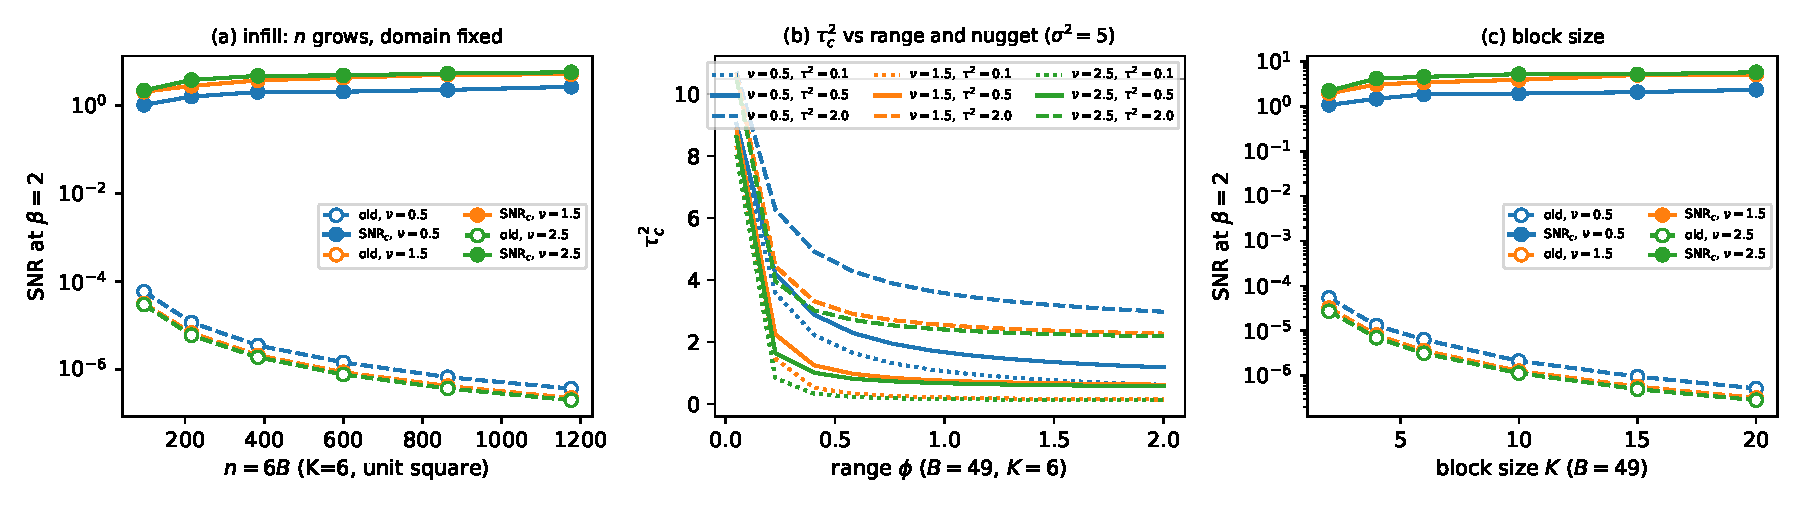
\includegraphics[width=\textwidth]{Figures/snr_comparison.pdf}
\caption{Old signal-to-noise ratio $\beta^2/(\lambda_{\max}(\bSig)\kappa(\bSig))$ (dashed) against the conditional one $\mathrm{SNR}_c=\Lambda/\tau_c^2$ (solid; $d=1$, $\Lambda=\beta^2\sigma_X^2$) on the simulation design of the submitted paper (unit square, $\sqrt B\times\sqrt B$ cells with $K$ uniform points each, $\sigma^2=5$, range $\phi=0.5$, $\tau^2=0.5$, $\sigma_X=1$, $\beta=2$) with Mat\'ern covariance of smoothness $\nu$ ($\nu=1/2$ is the exponential kernel of the paper). (a) Infill: $K=6$, $B$ from $16$ to $196$. (b) $\tau_c^2$ as a function of the range for three nuggets and three smoothnesses at $B=49$, $K=6$; the grey line is the bound $2\sigma^2+\tau^2$. (c) Block size $K$ at $B=49$. One random design per point.}
\label{fig:snr}
\end{figure}

\begin{definition}\label{def:constants}
Let $\bSig_{S\mid S^c}:=\bSig_{SS}-\bSig_{SS^c}\bSig_{S^cS^c}^{-1}\bSig_{S^cS}$ be the conditional covariance of $\bW^\ast_S$ given $\bW^\ast_{S^c}$, and
\[
\tau_c^2:=\max_b\max_{i\ne j\in\text{block }b}\lambda_{\max}\big(\bSig_{\{i,j\}\mid\{i,j\}^c}\big),\qquad\rho_c:=\tau^2/\tau_c^2,\qquad\mathrm{SNR}_c:=\Lambda/\tau_c^2=\beta^\top\bSig_X\beta/\tau_c^2 .
\]
For a common-key relabelling $\bR=\mathrm{bdiag}(\bm r,\dots,\bm r)$, $\bm r\in\calS_K$, let $\bSig_{\bR}:=\bR\bSig\bR^\top$ and
\begin{gather*}
\mu^2:=\max_{\bR}\lambda_{\max}(\bOm\bSig_{\bR}),\qquad\nu:=\max(\mu^2-1,1),\\
D(\bR):=\tfrac12[\tr(\bOm\bSig_{\bR})-n],\qquad\delta_{\mathrm{cov}}:=\min_{\bR\ne\bI}D(\bR)/\dH(\bR,\bI).
\end{gather*}
\end{definition}

\begin{lemma}\label{lem:constants}
(i) $\tau^2\le\tau_c^2\le2\sigma^2+\tau^2$. (ii) For $i\ne j$ in one block, $(\bm e_i\pm\bm e_j)^\top\bOm(\bm e_i\pm\bm e_j)\ge2/\tau_c^2$ and $\Omega_{ii}\ge1/\tau_c^2$; also $\|\bOm\|\le1/\tau^2$. (iii) With $\bM:=\bSig^{-1/2}\bR\bSig^{1/2}$ and $\bN:=\bM^\top\bM-\bI$: $\|\bM\|^2\le\mu^2$, $\|\bN\|\le\nu$, $\operatorname{rank}\bN\le2\dH(\bR,\bI)$, and $\tr\bN=2D(\bR)=2\,\mathrm{KL}(N(\bzero,\bSig_{\bR})\|N(\bzero,\bSig))\ge0$. (iv) $\mu^2\le(1+\sqrt{\Lambda_W/\tau^2})^2$ with $\Lambda_W:=\max_{\bR}\lambda_{\max}\Cov(\bR\bW-\bW)$.
\end{lemma}

\begin{theorem}[Common keys are recoverable]\label{thm:common}
Let Assumption~\ref{ass:dgp} hold with common keys, $\beta\ne\bzero$, $\bSig$ known, and let $(\hat\bPi_1,\hat\bPi_2)$ be \eqref{eq:ml}. Let $c$ be the Hanson--Wright constant of Lemma~\ref{lem:hw}, $c_d:=\tfrac15$ if $d=1$ and $c_d:=\tfrac1{10}$ if $d\ge2$, and put
\begin{gather*}
m_1:=\min\Big\{\frac{c_d\,\mathrm{SNR}_c}{32\mu^2},\frac{c\,c_d^2\,\mathrm{SNR}_c^2}{48K\nu^2},\frac{c\,c_d\,\mathrm{SNR}_c}{12\nu},\frac{c\rho_c^2}{16},\ \Big[\frac{c\rho_c^2}{32(d-1)^2},\frac{\rho_c}{32}\Big]_{d\ge2}\Big\},\\
m_2:=c\min\Big\{\frac{\delta_{\mathrm{cov}}^2}{6\nu^2},\frac{\delta_{\mathrm{cov}}}{3\nu}\Big\},
\end{gather*}
where the bracketed terms are present only for $d\ge2$; for $d=1$,
\[
m_1=\min\{\mathrm{SNR}_c/(160\mu^2),\ c\,\mathrm{SNR}_c^2/(1200K\nu^2),\ c\,\mathrm{SNR}_c/(60\nu),\ c\rho_c^2/16\}.
\]
If
\[
B\ \ge\ \max\Big\{\frac{2\log K}{m_1},\ \frac{2\log K}{m_2},\ \frac{4d\mu^2}{c_d\mathrm{SNR}_c},\ \frac{d\mu^2}{2\delta_{\mathrm{cov}}},\ 2d,\ \Big[\frac{64(d-1)}{K\rho_c}\Big]_{d\ge2}\Big\}
\]
then
\[
\Prob\big((\hat\bPi_1,\hat\bPi_2)\ne(\bPi_1,\bPi_2)\big)\le\{22+2d(d+1)\}K^{K+2}e^{-2Bm_1}+4K^2e^{-2Bm_2}.
\]
In the covariate-key sub-case ($\bpi_S=\bI$, so $\bR=\bI$, $\mu=1$ and only the first term occurs) the bound is $\{22+2d(d+1)\}K^2e^{-2Bm}$ with $m=\min\{c_d\mathrm{SNR}_c/32,\,c\rho_c^2/16,\,[c\rho_c^2/(32(d-1)^2),\rho_c/32]_{d\ge2}\}$ for $B\ge\max\{2\log K/m,\,4d/(c_d\mathrm{SNR}_c),\,[64(d-1)/(K\rho_c)]_{d\ge2}\}$.
\end{theorem}

\begin{corollary}[$\beta$ under a common key]\label{cor:beta-common}
Under the conditions of Theorem~\ref{thm:common}, on the event $\{\hat\bPi_2\bPi_2^\top\bPi_1\hat\bPi_1^\top=\bI\}$, whose complement has probability at most $\{22+2d(d+1)\}K^{K+2}e^{-2Bm_1}$, the profile estimator
\[
\hat\beta=(\bX^\top\hat\bPi_1^\top\bOm\hat\bPi_1\bX)^{-1}\bX^\top\hat\bPi_1^\top\bOm\hat\bPi_2\bY
\]
is conditionally unbiased with $\Cov(\hat\beta\mid\bX)\preceq\mu^2(\bX^\top\hat\bPi_1^\top\bOm\hat\bPi_1\bX)^{-1}$, and $\|\hat\beta-\beta\|=O_p\big(\tau_c\mu\sqrt{d/(n\lambda_{\min}(\bSig_X))}\big)$; for $d=1$ this is $O_p(\tau_c\mu/(\sigma_X\sqrt n))$, the submitted Theorem~2 with $\lambda_{\max}(\bSig)\kappa(\bSig)$ replaced by $\tau_c^2\mu^2$.
\end{corollary}

\begin{remark}\label{rem:common}
(a) On the simulation design of the submitted paper (unit square, $\sqrt B\times\sqrt B$ cells with $K$ uniform points each, $\sigma^2=5$, range $0.5$, $\tau^2=0.5$, $d=1$, $\sigma_X=1$): $\tau_c^2\in[1.3,2.3]$ and decreases with $B$, so $\mathrm{SNR}_c\approx2$--$3$ at $\beta=2$ and $28$--$50$ at $\beta=8$; $\mu^2\approx12$ ($K=6$) and $\approx30$ ($K=20$); $D(\bR)/B\approx1.4$ ($K=6$) and $\approx6.9$ ($K=20$), so $\delta_{\mathrm{cov}}\approx0.25$--$0.35$. Under fixed-domain sampling with a nugget, $\tau_c^2\to\tau^2$ (screening), $\Lambda_W$ stays bounded because the relabelling moves each point by at most a block diameter, and $\delta_{\mathrm{cov}}$ stays positive as long as no two points of a block coincide; under increasing-domain sampling all constants are fixed. The theorem is therefore a fixed-domain statement, which the submitted one was not.
(b) The constants $160$, $1200$ and the factor $K!$ absorbed in $K^{K+2}$ are crude and the bound is numerically far from the recovery observed at $B=49$, as such bounds are. Proposition~\ref{prop:free} in Appendix~\ref{app:common} gives the constants as functions of two free parameters $(\varepsilon,\gamma)$: for $d=1$ the choice $(0.2,0.3)$ replaces $160$ by $50$, $1200$ by $117$ and $60$ by $19$, at the price of $\rho_c^2/16\to\rho_c^2/100$ in the Hanson--Wright term.
(c) Case~2 of the proof (candidates that get the relative alignment right but the location key wrong) is exactly the location-key sub-case: recovery there is driven by the covariance signal $\delta_{\mathrm{cov}}$ alone, with no condition on $\beta$.
(d) Theorem~\ref{thm:common} and Theorem~\ref{thm:sep}(b)--(d) are the two ends of the mechanism design: re-use one key and the analyst recovers it at rate $e^{-cB}$; draw a fresh key per block and no adversary does better than the floors of \eqref{eq:floors}.
\end{remark}

\section{The full marginal likelihood: what is proved and what is not}\label{sec:full}

Theorem~\ref{thm:eff}(iii) is a statement about the composite likelihood \eqref{eq:composite}. This section records what can be said about the maximiser $\hat\beta_\rel$ of the full marginal likelihood \eqref{eq:marglik}, which is the object REPAIR approximates, and locates precisely the one step that is missing.

\subsection{Derivatives}
Write $\ell_\rel(\beta):=\log L_\rel(\beta)=\log\sum_{\bpi}w_{\bpi}e^{q_{\bpi}(\beta)}$ with $q_{\bpi}(\beta):=-\tfrac12(\bY-\bPi_X\bX\beta)^\top\bOm_{\bpi}(\bY-\bPi_X\bX\beta)-\tfrac12\log\det\bSig$, $\bOm_{\bpi}:=(\bPi_S\bSig_W\bPi_S^\top+\tau^2\bI)^{-1}$, and let $p_{\bpi}(\beta)\propto w_{\bpi}e^{q_{\bpi}(\beta)}$ be the key posterior. With the $d$-vector $\bS_{\bpi}:=\nabla_\beta q_{\bpi}=\bX^\top\bPi_X^\top\bOm_{\bpi}(\bY-\bPi_X\bX\beta)$ and the $d\times d$ matrix $\mathbf A_{\bpi}:=-\nabla^2_\beta q_{\bpi}=\bX^\top\bPi_X^\top\bOm_{\bpi}\bPi_X\bX$ (free of $\beta$),
\begin{equation}\label{eq:derivs}
\bm{\mathcal S}_\rel(\beta)=\nabla\ell_\rel(\beta)=\E_{p}[\bS_{\bpi}],\qquad \mathbf J_\rel(\beta):=-\nabla^2\ell_\rel(\beta)=\E_{p}[\mathbf A_{\bpi}]-\Cov_{p}(\bS_{\bpi}),
\end{equation}
and the third derivatives are $\partial_{\beta_k}\mathbf J_\rel=-\Cov_p(\mathbf A_{\bpi},S_{\bpi,k})-\partial_{\beta_k}\Cov_p(\bS_{\bpi})$, polynomials in posterior moments of $(\mathbf A_{\bpi},\bS_{\bpi})$ (Appendix~\ref{app:full}; for $d=1$, $\ell_\rel'''=-3\Cov_p(A_{\bpi},S_{\bpi})+\kappa_{3,p}(S_{\bpi})$ with $\kappa_{3,p}$ the third central moment under $p$). Two consequences are immediate. First, $\bOm_{\bpi}$ has the spectrum of $\bOm$ for every $\bpi$, so $\bX^\top\bX/\lambda_{\max}(\bSig)\preceq\mathbf A_{\bpi}\preceq\bX^\top\bX/\tau^2$ deterministically, and the same bounds hold for $\E_p[\mathbf A_{\bpi}]$: the ``expected-Hessian'' part of the observed information is of exact order $n$ (its eigenvalues lie between $\lambda_{\min}(\bX^\top\bX)/\lambda_{\max}(\bSig)$ and $\lambda_{\max}(\bX^\top\bX)/\tau^2$) whatever the posterior does. Second, $\mathbf J_\rel$ can be smaller than $\E_p[\mathbf A_{\bpi}]$ by the posterior covariance of the score, and can fail to be positive definite: $\ell_\rel$ is not concave in $\beta$. On the simulation design this shows up as a second local maximum of the likelihood near $-\beta$ (Section~\ref{sec:numerics}), which is why the estimator to analyse is the local maximiser near a consistent starting point, not the global one.

\subsection{Increasing domain: the precision matrix is local and the informations are of order $B$}

\begin{lemma}[Locality of the precision]\label{lem:decay}
Let the locations be $\delta$-separated in $\mathbb R^2$ and $|C_W(h)|\le c_0(1+\|h\|)^{-\gamma}$ with $\gamma>2$ (Assumption~\ref{ass:mixing}(ii)), $\tau^2>0$. Then
(i) $M:=\sup_i\sum_j|(\bSig_W)_{ij}|\le c_0c_\delta\sum_{r\ge0}(1+r)^{1-\gamma}<\infty$, with $c_\delta$ depending only on $\delta$, so $\tau^2\le\lambda_{\min}(\bSig)\le\lambda_{\max}(\bSig)\le\tau^2+M$ uniformly in $n$;
(ii) $|\Omega_{ij}|\le C_1(1+\|s_i-s_j\|)^{-\gamma}$ for all $i,j$, with $C_1$ depending only on $c_0,\gamma,\delta,\tau^2$;
(iii) for blocks $b\ne b'$ at minimal point distance $d_{bb'}$, $\|\bOm_{bb'}\|\le\|\bOm_{bb'}\|_F\le\bar KC_1(1+d_{bb'})^{-\gamma}$.
\end{lemma}
Part (ii) is Jaffard's theorem on the inverse-closedness of matrices with polynomial off-diagonal decay over relatively separated index sets (Jaffard 1990; Gr\"ochenig and Leinert 2006; Sun 2007). It says that under increasing-domain sampling the likelihood weights $\bOm$ couple a block only to its neighbours, with a coupling that decays like the covariance itself.

\begin{proposition}[Order of the three informations]\label{prop:order}
Under Lemma~\ref{lem:decay}, with $K_{\min}\le K_b\le\bar K$,
\[
\frac{K_{\min}B}{\bar K(\tau^2+M)}\,\bSig_X\ \preceq\ \mathbf I_\agg\ \preceq\ \mathbf I_\rel\ \preceq\ \mathbf I_\orc\ \preceq\ \frac{\bar KB}{\tau^2}\,\bSig_X,
\qquad\text{so}\qquad \bI_d\preceq\mathbf I_\agg^{-1/2}\mathbf I_\rel\mathbf I_\agg^{-1/2}\preceq\frac{\bar K^2(\tau^2+M)}{K_{\min}\tau^2}\,\bI_d .
\]
\end{proposition}
All three informations grow linearly in $B$, and the efficiency gain of the marginal likelihood over the areal GLS is a bounded factor under increasing-domain sampling; under fixed-domain sampling $M$ grows with $n$ and the factor can grow (the $K=6$ table of Remark~\ref{rem:eff} is the fixed-domain case).

\subsection{Asymptotics under two conditions}
Let $\mathbf I:=\mathbf I_\rel(\beta_0)$, whose smallest eigenvalue tends to infinity by Proposition~\ref{prop:order}, and write $\mathcal N_C:=\{\beta:\|\mathbf I^{1/2}(\beta-\beta_0)\|\le C\}$ for the $\mathbf I$-standardised ball of radius $C$. Consider
\begin{itemize}
\item[(C1)] $\mathbf I^{-1/2}\bm{\mathcal S}_\rel(\beta_0)\rightsquigarrow N_d(\bzero,\bI_d)$;
\item[(C2)] for every $C>0$, $\sup_{\beta\in\mathcal N_C}\|\mathbf I^{-1/2}\mathbf J_\rel(\beta)\mathbf I^{-1/2}-\bI_d\|\to0$ in probability.
\end{itemize}
By Theorem~\ref{thm:eff}(ii) and the Fisher identity, $\E\bm{\mathcal S}_\rel(\beta_0)=\bzero$ and $\Cov\bm{\mathcal S}_\rel(\beta_0)=\mathbf I$ exactly, so (C1) asks only for the shape of the distribution of a statistic whose first two moments are known; (C2) is a local law of large numbers for the observed information.

\begin{theorem}[Local maximiser and one-step estimator]\label{thm:onestep}
Assume (C1)--(C2). (a) For every $\eta>0$ there is $C<\infty$ such that, with probability at least $1-\eta$ for all large $B$, $\ell_\rel$ has exactly one stationary point $\hat\beta_\rel$ in $\mathcal N_C$, it is a local maximum, and $\mathbf I^{1/2}(\hat\beta_\rel-\beta_0)\rightsquigarrow N_d(\bzero,\bI_d)$.
(b) Let $\tilde\beta$ be any estimator with $\mathbf I^{1/2}(\tilde\beta-\beta_0)=O_p(1)$, for instance the areal GLS $\hat\beta_\agg$ or the composite maximiser. The one-step estimator $\hat\beta_1:=\tilde\beta+\mathbf J_\rel(\tilde\beta)^{-1}\bm{\mathcal S}_\rel(\tilde\beta)$ satisfies $\mathbf I^{1/2}(\hat\beta_1-\hat\beta_\rel)\to\bzero$ in probability, hence $\mathbf I^{1/2}(\hat\beta_1-\beta_0)\rightsquigarrow N_d(\bzero,\bI_d)$.
(c) Consequently the asymptotic covariance of $\hat\beta_\rel$ is $\mathbf I_\rel^{-1}\preceq\mathbf I_\agg^{-1}$, the areal GLS covariance, with $\mathbf I_\agg^{1/2}\mathbf I_\rel^{-1}\mathbf I_\agg^{1/2}\preceq\bI_d$ measuring the gain.
The same statements hold for the composite likelihood with $\ell_{\mathrm{cl}}$, $\mathbf I_{\mathrm{cl}}:=\sum_b\mathbf I_b$ in place of $\ell_\rel,\mathbf I$; Theorem~\ref{thm:eff}(iii) is precisely the verification of (C1)--(C2) for $\ell_{\mathrm{cl}}$ under Assumption~\ref{ass:mixing}.
\end{theorem}

\begin{remark}[Where the obstacle is]\label{rem:obstacle}
For the composite likelihood, $\bm{\mathcal S}_{\mathrm{cl}}(\beta_0)=\sum_b\nabla_\beta\log f_b(\bY_b;\beta_0)$ is a sum of block functionals and (C1)--(C2) follow from the mixing central limit theorem. For the full likelihood, $\bm{\mathcal S}_\rel(\beta_0)=\sum_b\E_p[\bS_{\bpi,b}]$ with $\bS_{\bpi,b}:=\bX_b^\top\bpi_X^{(b)\top}[\bOm_{\bpi}(\bY-\bPi_X\bX\beta_0)]_b$, and the expectation is under the key posterior, which is a Gibbs measure on $\prod_b(\calS_{K_b}\times\calS_{K_b})$: in the covariate-key sub-case its energy is $-q_{\bpi}=\tfrac12\sum_b\bm r_b^\top\bOm_{bb}\bm r_b+\tfrac12\sum_{b\ne b'}\bm r_b^\top\bOm_{bb'}\bm r_{b'}$ with block residuals $\bm r_b=\bY_b-\bpi_X^{(b)}\bX_b\beta_0$, so the keys of different blocks interact through $\bOm_{bb'}$, which decays like $(1+d_{bb'})^{-\gamma}$ by Lemma~\ref{lem:decay}. A central limit theorem for $\sum_b\E_p[\bS_{\bpi,b}]$ requires the posterior correlation between the keys of distant blocks to decay, i.e.\ a Dobrushin-type uniqueness condition for this Gibbs measure, whose interaction strengths $\|\beta_0\|\,\|\bOm_{bb'}\|\,\|\bX_b\|\,\|\bm r_{b'}\|$ are data-dependent and not uniformly small. Establishing that condition on an event of probability tending to one is the missing step; the composite likelihood is the case in which the interactions are set to zero. What the present section does establish is that the target has the right order ($\mathbf I\asymp B\,\bSig_X$), that the observed information has a deterministic expected-Hessian part of exact order $n$, and that once (C1)--(C2) hold, one Newton step from the areal estimator attains the efficiency $\mathbf I_\rel$.
\end{remark}

\section{Numerical checks}\label{sec:numerics}

All computations use the simulation design of the submitted paper (unit square, $\sqrt B\times\sqrt B$ cells with $K$ uniform points each, $\sigma^2=5$, $\tau^2=0.5$, one covariate with $\sigma_X=1$, exponential kernel with range $0.5$ unless stated), keys drawn independently and uniformly in every block. Code: \texttt{sims/simA\_constants.py}, \texttt{simB\_relink.py}, \texttt{simC\_estimators.py} next to this file.

\subsection{Constants of Theorem~\ref{thm:common} and the composite information on Mat\'ern designs}
Table~\ref{tab:constants} gives, for $B=49$, $K=6$ and one random design, the constants of Definition~\ref{def:constants} computed exactly ($\mu^2$, $\delta_{\mathrm{cov}}$ and $\max_{\bR}D(\bR)/B$ by enumerating the $6!$ common-key relabellings), together with the ratio $I_{\mathrm{cl}}/I_\agg$ of the composite information $\sum_bI_b$ (covariate-key sub-case, $I_b$ by Monte Carlo over $150$ draws per block) to the areal information $\sigma_X^2\tr(\bV^{-1}\bD)$, and the fraction $I_{\mathrm{cl}}/I_\orc$ of the oracle information the composite likelihood retains at $\beta=1$.

\begin{table}[t]\centering\small
\begin{tabular}{cccrrrrrrrr}\toprule
$\nu$ & $\phi$ & $\tau^2$ & $\tau_c^2$ & $\mu^2$ & $\delta_{\mathrm{cov}}$ & $\max D/B$ & \multicolumn{3}{c}{$I_{\mathrm{cl}}/I_\agg$ at $\beta=0.5,1,2$} & $I_{\mathrm{cl}}/I_\orc$ ($\beta=1$)\\\midrule
0.5 & 0.25 & 0.5 & 5.32 & 14.5 & 0.270 & 1.97 & 8.2 & 14.9 & 18.9 & 0.56\\
0.5 & 0.5  & 0.5 & 3.39 & 14.5 & 0.216 & 1.53 & 7.9 & 13.3 & 16.1 & 0.61\\
0.5 & 1.0  & 0.5 & 2.15 & 11.5 & 0.140 & 0.99 & 6.9 & 11.0 & 12.8 & 0.65\\
1.5 & 0.25 & 0.5 & 3.03 & 35.1 & 0.473 & 3.33 & 9.6 & 15.3 & 17.5 & 0.58\\
1.5 & 0.5  & 0.5 & 1.43 & 24.4 & 0.188 & 1.44 & 5.5 & 8.3 & 9.4 & 0.66\\
1.5 & 1.0  & 0.5 & 0.87 & 13.6 & 0.057 & 0.46 & 4.0 & 6.2 & 6.9 & 0.70\\
2.5 & 0.25 & 0.5 & 2.30 & 42.1 & 0.468 & 3.40 & 7.6 & 11.3 & 13.0 & 0.59\\
2.5 & 0.5  & 0.5 & 1.11 & 24.6 & 0.149 & 1.18 & 4.2 & 6.4 & 7.3 & 0.67\\
2.5 & 1.0  & 0.5 & 0.72 & 12.9 & 0.041 & 0.33 & 3.5 & 5.4 & 5.9 & 0.71\\
0.5 & 0.5  & 0.1 & 2.81 & 28.6 & 0.491 & 3.68 & 17.2 & 22.7 & 25.6 & 0.62\\
0.5 & 0.5  & 2.0 & 5.31 & 6.3 & 0.064 & 0.45 & 2.6 & 6.0 & 9.2 & 0.47\\\bottomrule
\end{tabular}
\caption{Constants on the simulation design ($B=49$, $K=6$) for Mat\'ern smoothness $\nu$, range $\phi$ and nugget $\tau^2$. $\mu^2$, $\delta_{\mathrm{cov}}$ and $D(\bR)$ are those of Definition~\ref{def:constants}; $I_{\mathrm{cl}}/I_\agg$ is the predicted efficiency gain of the composite-likelihood estimator over areal GLS (Theorem~\ref{thm:onestep}(c)); $I_{\mathrm{cl}}/I_\orc$ the share of the oracle information retained.}
\label{tab:constants}
\end{table}

Three things stand out. The covariance-shift constants $\mu^2$ and $\delta_{\mathrm{cov}}$ move together and are driven by how much a within-block relabelling changes the covariance: smoother fields and shorter ranges make the relabelling more visible ($\delta_{\mathrm{cov}}$ up to $0.49$), long ranges and large nuggets make it nearly invisible ($\delta_{\mathrm{cov}}=0.04$ at $\nu=2.5$, $\phi=1$), so the location key is easy to recover in the first case and hard in the second, independently of $\beta$. The gain of the composite likelihood over areal GLS is between $3$ and $26$ on this design and increases with $\beta$ and with the field-to-nugget ratio: the areal estimator loses because block sums are dominated by the field, and the within-block contrasts, which the composite likelihood uses and the block sums discard, have residual variance only $\tau_c^2$. The composite likelihood retains $47$--$71\%$ of the oracle information at $\beta=1$; the rest is the information carried by the keys (Theorem~\ref{thm:eff}(ii)).

\subsection{Re-linking rates against the floors of Theorem~\ref{thm:sep}}
Table~\ref{tab:relink} reports, for $B=49$, $K=6$ and $100$ replications, the per-block error rate of the Bayes-optimal adversary of Theorem~\ref{thm:sep}(b): for the covariate key it knows $\bX$, $\bW$ at the released locations and every other key, and chooses among the $720$ candidates by least squares (``strong''); a second adversary does not know $\bW$ and uses the block-marginal Gaussian likelihood (``marginal''). The floors are $p^X$ of \eqref{eq:pX} and, for the fraction of misplaced records, the refined bound $p^X(1-B/n)$ of Theorem~\ref{thm:sep}(c). For the location key the strong adversary knows $\bX$, $\beta$ and the multiset of $\bW$-values of the block.

\begin{table}[t]\centering\small
\begin{tabular}{crrrrrrrr}\toprule
 & \multicolumn{5}{c}{covariate key ($\bpi_S=\bI$)} & \multicolumn{2}{c}{location key ($\bpi_X=\bI$)}\\
\cmidrule(lr){2-6}\cmidrule(lr){7-8}
$\beta$ & floor $p^X$ & strong & marginal & floor misplaced & misplaced (strong) & floor $\bar p^S$ & strong\\\midrule
0.25 & 0.392 & 0.993 & 0.997 & 0.327 & 0.774 & 0.336 & 0.956\\
0.5  & 0.304 & 0.986 & 0.990 & 0.253 & 0.707 & 0.336 & 0.963\\
1    & 0.196 & 0.937 & 0.971 & 0.163 & 0.577 & 0.336 & 0.959\\
2    & 0.108 & 0.791 & 0.885 & 0.090 & 0.395 & 0.336 & 0.958\\
4    & 0.056 & 0.551 & 0.678 & 0.046 & 0.229 & 0.336 & 0.960\\
8    & 0.028 & 0.340 & 0.457 & 0.023 & 0.129 & 0.336 & 0.960\\\bottomrule
\end{tabular}
\caption{Per-block probability that the estimated key is wrong, and expected fraction of records placed at a wrong position, for the adversaries described in the text ($B=49$, $K=6$, $\tau^2=0.5$, $\sigma_X=1$), next to the lower bounds of Theorem~\ref{thm:sep}. $\bar p^S$ is the floor $\max_{i\ne j}p^S_{b,ij}$ averaged over blocks (its minimum over blocks is $0.278$). The all-keys bound $(1-p^X)^B$ is $0.004$ at $\beta=2$ and $0.25$ at $\beta=8$; no replication recovered all $49$ covariate keys at any $\beta$.}
\label{tab:relink}
\end{table}

The floors are lower bounds for a two-point test, so they are below the actual error of an adversary facing $720$ candidates, by a factor of $2.5$ ($\beta=0.25$) to $12$ ($\beta=8$) for the per-block error and by a factor of $2.4$ to $5.6$ for the misplaced fraction. Two qualitative predictions of Theorem~\ref{thm:sep} are visible: the covariate-key risk decreases with $|\beta|/\tau$ exactly as $\arctan(\tau/(|\beta|\sigma_X))$ does, and the location-key risk does not depend on $\beta$ at all and stays near $0.96$ per block on this design, where the floor is $0.34$. Even at $\beta=8$, sixteen times the noise standard deviation, a third of the blocks are re-linked wrongly and $13\%$ of records are misplaced, while by Theorem~\ref{thm:sep}(a) and Table~\ref{tab:estimators} $\beta$ is estimated to within a few percent.

\subsection{Composite-likelihood estimator against areal GLS and the oracle}
Table~\ref{tab:estimators} compares, for $K=4$ (so that the $4!^2=576$ key configurations of a block can be enumerated exactly), the areal GLS $\hat\beta_\agg$, the oracle GLS with the true keys, and the composite-likelihood estimator of \eqref{eq:composite}, in the covariate-key sub-case and in the general case with independent covariate and location keys; $150$ replications. Two versions of the composite estimator are shown: the global maximiser over $[-4,4]$ (grid of step $0.05$, then refined), and the local maximiser started at $\hat\beta_\agg$ and searched within three areal standard errors of it, which is the estimator Theorem~\ref{thm:onestep} is about.

\begin{table}[t]\centering\footnotesize
\begin{tabular}{ccc rrr rr r rr}\toprule
case & $B$ & $\beta$ & areal & oracle & \multicolumn{2}{c}{comp.\ global} & comp.\ local & $1/I_{\mathrm{cl}}$ & \multicolumn{2}{c}{areal/local}\\
 & & & MSE & MSE & MSE & wrong sign & MSE & & emp. & $I_{\mathrm{cl}}/I_\agg$\\\midrule
X & 25 & 0.5 & 0.141 & 0.015 & 0.267 & 0.25 & 0.142 & 0.034 & 1.0 & 4.2\\
X & 25 & 1   & 0.137 & 0.016 & 0.345 & 0.08 & 0.045 & 0.023 & 3.1 & 6.5\\
X & 25 & 2   & 0.150 & 0.014 & 0.019 & 0.00 & 0.018 & 0.018 & 8.2 & 8.0\\
X & 49 & 0.5 & 0.067 & 0.005 & 0.244 & 0.24 & 0.068 & 0.014 & 1.0 & 4.0\\
X & 49 & 1   & 0.067 & 0.006 & 0.009 & 0.00 & 0.009 & 0.009 & 7.9 & 6.3\\
X & 49 & 2   & 0.071 & 0.006 & 0.008 & 0.00 & 0.008 & 0.008 & 8.6 & 7.1\\
X & 100 & 0.5 & 0.018 & 0.003 & 0.088 & 0.09 & 0.007 & 0.006 & 2.6 & 3.4\\
X & 100 & 1   & 0.017 & 0.003 & 0.004 & 0.00 & 0.004 & 0.004 & 4.5 & 5.9\\
X & 100 & 2   & 0.020 & 0.003 & 0.004 & 0.00 & 0.004 & 0.003 & 5.6 & 6.7\\\midrule
G & 25 & 0.5 & 0.131 & 0.013 & 0.178 & 0.13 & 0.121 & 0.046 & 1.1 & 3.4\\
G & 25 & 1   & 0.195 & 0.012 & 0.237 & 0.05 & 0.103 & 0.025 & 1.9 & 5.9\\
G & 25 & 2   & 0.147 & 0.014 & 0.020 & 0.00 & 0.020 & 0.019 & 7.3 & 8.0\\
G & 49 & 0.5 & 0.069 & 0.005 & 0.160 & 0.14 & 0.061 & 0.018 & 1.1 & 3.0\\
G & 49 & 1   & 0.057 & 0.005 & 0.034 & 0.01 & 0.012 & 0.010 & 4.9 & 5.5\\
G & 49 & 2   & 0.059 & 0.006 & 0.008 & 0.00 & 0.008 & 0.008 & 7.2 & 6.9\\
G & 100 & 0.5 & 0.020 & 0.002 & 0.115 & 0.12 & 0.011 & 0.007 & 1.8 & 3.1\\
G & 100 & 1   & 0.023 & 0.002 & 0.004 & 0.00 & 0.004 & 0.004 & 6.2 & 5.3\\
G & 100 & 2   & 0.025 & 0.003 & 0.004 & 0.00 & 0.004 & 0.003 & 6.7 & 6.8\\\bottomrule
\end{tabular}
\caption{Mean squared errors over $150$ replications, $K=4$; X: covariate key only, G: both keys independent. ``Wrong sign'' is the fraction of replications in which the global composite maximiser has the wrong sign. $1/I_{\mathrm{cl}}$ is the asymptotic variance of Theorem~\ref{thm:onestep} for the composite likelihood, with $I_{\mathrm{cl}}$ the Monte Carlo mean of the observed composite information at $\beta_0$. The last two columns compare the empirical MSE ratio areal/local with the information ratio $I_{\mathrm{cl}}/I_\agg$.}
\label{tab:estimators}
\end{table}

Three conclusions. First, once $|\beta|\ge1$ and $B\ge49$ the local composite estimator's MSE equals $1/I_{\mathrm{cl}}$ to within Monte Carlo error and its gain over areal GLS matches $I_{\mathrm{cl}}/I_\agg$ ($4.5$--$8.6$ observed against $5.3$--$7.1$ predicted), which is Theorem~\ref{thm:onestep}(c) for the composite likelihood; the areal MSE itself is between a sixth and an eleventh of the crude bound $(K\sigma^2+\tau^2)/(\sigma_X^2(B-2))$ of \eqref{eq:mse}, and six to thirteen times the oracle MSE. Second, the composite likelihood is bimodal in $\beta$ with a second local maximum near $-\beta_0$: at $\beta_0=0.5$ the global maximiser picks the wrong sign in $9$--$25\%$ of replications and is then worse than areal GLS, whereas the local maximiser started at $\hat\beta_\agg$ is never worse than areal GLS and is $1.8$--$2.6$ times better at $B=100$. This is the practical content of Theorem~\ref{thm:onestep}(b) and the reason to anchor the algorithm at the areal estimator: the sign of $\beta$ is identified by the block sums, which are almost uninformative about the keys, and the within-block contrasts add precision but not sign. Third, at $\beta_0=0.5$ and $B\le49$ the local estimator is only as good as the areal one although $I_{\mathrm{cl}}/I_\agg\approx3$--$4$: the asymptotic regime of Theorem~\ref{thm:onestep} needs $I_{\mathrm{cl}}^{-1/2}$ small compared with the distance $2|\beta_0|$ between the two modes, i.e.\ $|\beta_0|\sqrt{I_{\mathrm{cl}}}$ large, which is $2.7$ at $B=25$ and $6$ at $B=100$.

\subsection{Which key, which direction, which covariate: the information share by exact enumeration}\label{sec:infochecks}

Figure~\ref{fig:infochecks} isolates, by exact enumeration of the keys in a single block ($K=4$ or $5$, $W_b$ integrated out, $200$--$400$ random blocks of the simulation design), the share $\mathbf I_b/\mathbf I_b^{\orc}$ of the oracle information that the block-marginal likelihood retains, next to the corresponding floor of Theorem~\ref{thm:sep}.

\emph{(a) Which key is unknown.} With the covariate key known and only the location key unknown, the share is flat in $\beta$ at about $0.9$: not knowing where the responses sit costs the analyst only the correct GLS weighting within the block, and the loss does not depend on the effect size, exactly as the floor $p^S$, which does not involve $\beta$, is flat. With the covariate key unknown the share rises from near $0$ at $\beta=0.1$ to $0.95$ at $\beta=4$ as $p^X$ falls from $0.47$ to $0.06$: the information the analyst gains and the re-linking risk the record incurs are two readings of the same key posterior. Unknown location key on top of an unknown covariate key costs almost nothing further (the ``both keys'' curve sits on the ``covariate key'' curve), and the single-key case is slightly better at small $\beta$ because the field shift adds to the covariate shift in the two-point problem ($p^{XS}<p^X$). The location key is therefore the cheap key to scramble: it is protected by a $\beta$-free floor and it is nearly free for the analyst.

\emph{(b) Several covariates.} Along the direction of $\beta$ the share depends on $(\beta,\bSig_X)$ only through $\Lambda=\beta^\top\bSig_X\beta$, and the curves for $d=1,2,3$ coincide, as Theorem~\ref{thm:sep} and Theorem~\ref{thm:eff}(i) predict. In directions orthogonal to $\beta$ the share is lower, roughly half, at every $\Lambda$. This is a genuine feature, not noise: the key posterior is learned from the linear predictor $\bX\beta$ alone, so a covariate column that does not enter the linear predictor is aligned only to the extent that the key is, while its own contrasts contribute nothing to identifying the key. Theorem~\ref{thm:eff}(i) is consistent with this ($\mathbf I_\orc$ and $\mathbf I_\agg$ are multiples of $\bSig_X$, and $\mathbf I_\rel$ lies between them), but $\mathbf I_\rel$ itself is not a multiple of $\bSig_X$: the released data are most informative about $\beta$ in the direction of $\beta$.

\emph{(c) A covariate field independent of $W$.} In the single-key case with $X$ an exponential field of range $0.3$ or $0.1$ read at the true location, the share curve is the i.i.d.\ curve shifted to the right in $\beta$ by the factor $\sqrt{v^g/2}$ of Section~\ref{sec:spatialX} (a within-block variogram of $0.4$ at range $0.3$ moves $\beta=4$ to an effective $1.8$), and the floor $p^X$ of \eqref{eq:pX-g} shifts with it. That is why the gains over areal GLS in Table~\ref{tab:realistic} are modest for a smooth covariate: the effective signal is smaller, and in addition the areal estimator is itself close to the oracle when $X$ varies little within a block (Table~\ref{tab:spatialX}), so the ceiling on the gain is low. Nothing here depends on $g$ being dependent on $W$; the two fields are independent throughout.

\begin{figure}[t]
\centering
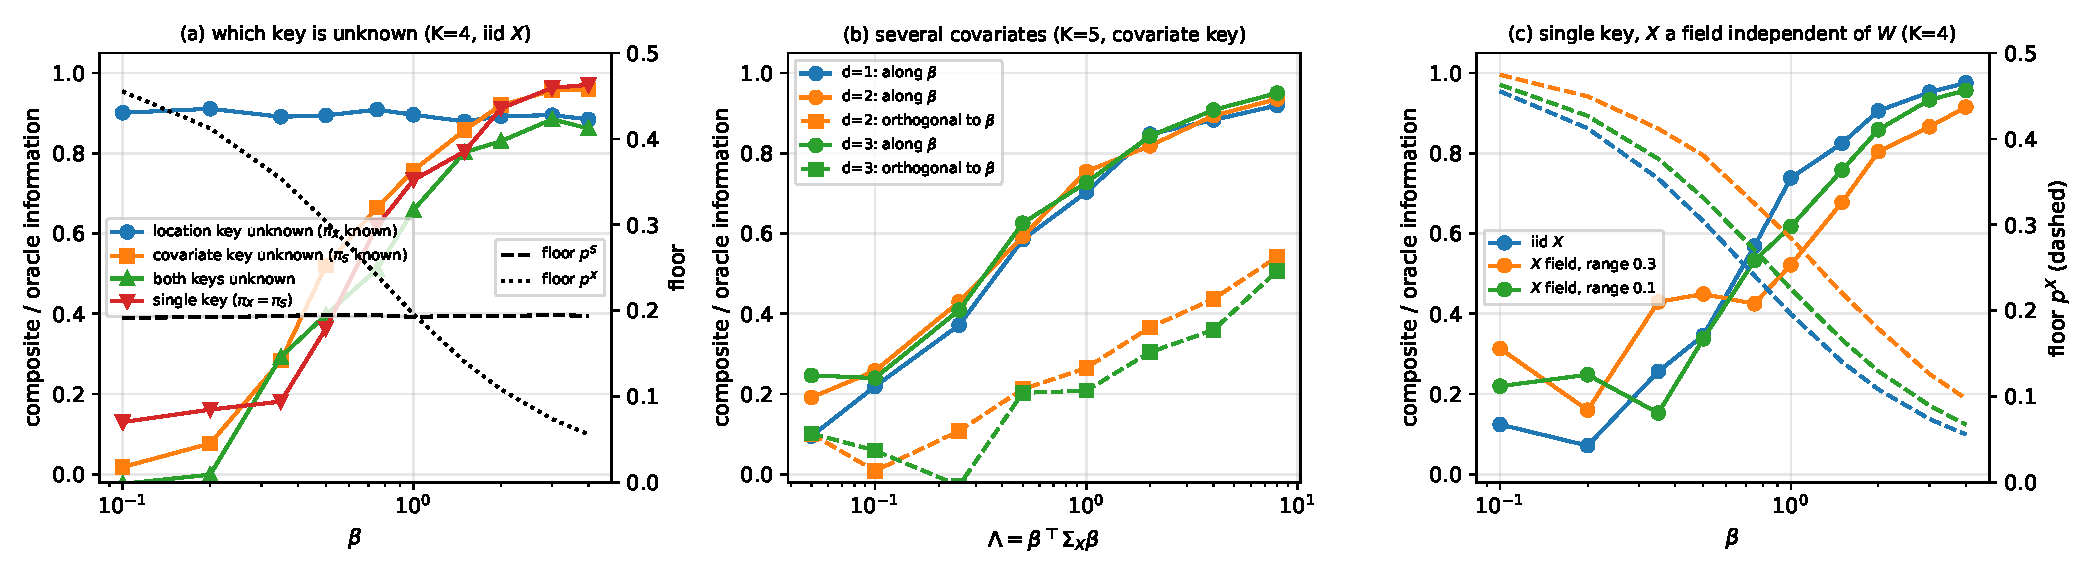
\includegraphics[width=\textwidth]{Figures/info_checks.pdf}
\caption{Share of the oracle information retained by the block-marginal likelihood, by exact enumeration of the keys ($\sigma^2=5$, range $0.5$, $\tau^2=0.5$, $\sigma_X=1$; block = one cell of the $7\times7$ design). (a) $K=4$, i.i.d.\ $X$, by which key is unknown; right axis: the floors $p^S$ (dashed) and $p^X$ (dotted). (b) $K=5$, covariate key unknown, $d=1,2,3$ covariates with $\bSig_X=\tfrac12(\bI+\bone\bone^\top)$ for $d\ge2$, against $\Lambda$; solid: share along $\beta$, dashed: average share over directions orthogonal to $\beta$. (c) $K=4$, single key, $X$ i.i.d.\ or an exponential field of range $0.3$ or $0.1$ independent of $W$; dashed: the floor $p^X$ of \eqref{eq:pX-g}. Script \texttt{sims/info\_checks.py}.}
\label{fig:infochecks}
\end{figure}

\subsection{An estimator for realistic block sizes: the areal-augmented composite likelihood}\label{sec:realistic}

Table~\ref{tab:estimators} enumerates the $K!^2$ key configurations of a block, which is possible only for $K\le5$. Real blocks are larger (clusters of $20$--$40$ households, plates of $96$ wells), so the estimator that goes into the code must approximate the per-block sum over keys, and the composite likelihood alone turns out to lose something specific at large $K$: the block sums are then dominated by the field, so the sign of $\beta$, which the within-block contrasts do not identify, is carried almost entirely by the \emph{between-block} covariance of the sums, which \eqref{eq:composite} discards. Both problems are fixed by one construction. Write $f_b(\bY_b)=f_b(T_b)\,f_b(\bY_b\mid T_b)$; the block sum is key-invariant, so $f_b(T_b;\beta)=\phi(T_b;\bS_b^\top\beta,V_{bb})$ involves no keys. Replace the product of the $B$ independent sum densities by the joint GLS density of all sums:
\begin{equation}\label{eq:aug}
\begin{aligned}
\ell^\ast(\beta)&:=\log\phi_B(\bT;\mathbf S\beta,\bV)+\sum_{b=1}^B\big[\log f_b(\bY_b;\beta)-\log\phi(T_b;\bS_b^\top\beta,V_{bb})\big]\\
&=\ell_{\mathrm{cl}}(\beta)+\Big[\ell_{\mathrm{GLS}}(\bT;\beta)-\sum_b\ell_b(T_b;\beta)\Big].
\end{aligned}
\end{equation}
This is again a composite likelihood in Lindsay's sense (one marginal component for $\bT$, $B$ conditional components), so Theorem~\ref{thm:onestep} applies to it with the same mixing argument, its score is $\bm{\mathcal S}^\ast=\bm{\mathcal S}_{\mathrm{cl}}+\mathbf S^\top\bV^{-1}(\bT-\mathbf S\beta)-\sum_b\bS_b(T_b-\bS_b^\top\beta)/V_{bb}$, and its information is $\mathbf I^\ast=\mathbf I_{\mathrm{cl}}+\mathbf I_\agg-\sum_b\mathbf I_b^{\mathrm{sum}}\succeq\max(\mathbf I_{\mathrm{cl}},\mathbf I_\agg)$ in the Loewner sense, because each block marginal dominates its own sum coarsening (Step~3 of the proof of Theorem~\ref{thm:eff}). The bracket in \eqref{eq:aug} is explicit; only $\bm{\mathcal S}_{\mathrm{cl}}$ needs the key posterior, and by \eqref{eq:derivs} applied block by block it is $\sum_b\E_{p_b}[\tilde{\bX}_b^\top\bOm_b\bm r_b]$, a posterior mean under the $K_b!^2$-point key posterior of block $b$, with $\tilde{\bX}_b$ the rows of $\bX_b$ in the posterior key order and $\bm r_b$ the aligned residual.

\emph{Computation.} Per block, given $\beta$, a Metropolis chain over the two keys with transposition proposals, each costing $O(K_b)$ through the block precision $\bOm_b$, returns $\E_{p_b}[\tilde{\bX}_b^\top\bOm_b\bm r_b]$ and $\E_{p_b}[\tilde{\bX}_b^\top\bOm_b\tilde{\bX}_b]$; the blocks are independent given $\beta$, so this parallelises, and for $K_b\le5$ the chain can be replaced by enumeration. Then a damped Newton step $\beta\leftarrow\beta+\mathbf M^{-1}\bm{\mathcal S}^\ast$ with the positive-definite preconditioner $\mathbf M=\sum_b\E_{p_b}[\tilde{\bX}_b^\top\bOm_b\tilde{\bX}_b]+\mathbf S^\top\bV^{-1}\mathbf S\succeq\mathbf I^\ast$, started at $\hat\beta_\agg$, iterated ten times. The covariance parameters are those of the areal stage, which sees all between-block distances; the composite terms see only within-block ones. One fit costs about one second at $B=100$, $\bar K=30$ on one core (\texttt{sims/simE3\_aug.py}; the variational relaxation of the submitted paper can play the same role as the chain, with the chain and, at $K\le5$, enumeration as its check).

\begin{table}[t]\centering\footnotesize\setlength{\tabcolsep}{4pt}
\begin{tabular}{lcccc rrr rrr}\toprule
keys & $B$ & $\bar K$ & $\nu$ & $\beta$ & areal & oracle & augm. & areal/augm. & oracle/augm. & wrong sign\\\midrule
both keys & 64 & 20 & 0.5 & 0.25 & 0.1306 & 0.0007 & 0.0758 & 1.7 & 0.01 & 0.25\\
both keys & 64 & 20 & 0.5 & 0.50 & 0.1306 & 0.0007 & 0.0898 & 1.5 & 0.01 & 0.10\\
both keys & 64 & 20 & 0.5 & 1.00 & 0.1306 & 0.0007 & 0.0014 & 95.2 & 0.48 & 0.00\\
both keys & 64 & 20 & 0.5 & 2.00 & 0.1306 & 0.0007 & 0.0010 & 133.4 & 0.67 & 0.00\\
both keys & 100 & 30 & 0.5 & 0.25 & 0.0959 & 0.0002 & 0.0510 & 1.9 & 0.00 & 0.25\\
both keys & 100 & 30 & 0.5 & 0.50 & 0.0959 & 0.0002 & 0.0753 & 1.3 & 0.00 & 0.07\\
both keys & 100 & 30 & 0.5 & 1.00 & 0.0735 & 0.0002 & 0.0005 & 163.0 & 0.45 & 0.00\\
both keys & 100 & 30 & 0.5 & 2.00 & 0.0735 & 0.0002 & 0.0003 & 266.5 & 0.74 & 0.00\\
both keys & 64 & 20 & 1.5 & 1.00 & 0.0249 & 0.0005 & 0.0012 & 20.9 & 0.42 & 0.00\\
covariate key & 64 & 20 & 0.5 & 0.25 & 0.0705 & 0.0006 & 0.0406 & 1.7 & 0.01 & 0.17\\
covariate key & 64 & 20 & 0.5 & 0.50 & 0.0705 & 0.0006 & 0.0429 & 1.6 & 0.01 & 0.04\\
covariate key & 64 & 20 & 0.5 & 1.00 & 0.0705 & 0.0006 & 0.0008 & 85.8 & 0.69 & 0.00\\
covariate key & 64 & 20 & 0.5 & 2.00 & 0.0705 & 0.0006 & 0.0009 & 82.9 & 0.67 & 0.00\\
covariate key & 100 & 30 & 0.5 & 0.25 & 0.0647 & 0.0002 & 0.0526 & 1.2 & 0.00 & 0.25\\
covariate key & 100 & 30 & 0.5 & 0.50 & 0.0647 & 0.0002 & 0.0367 & 1.8 & 0.01 & 0.04\\
covariate key & 100 & 30 & 0.5 & 1.00 & 0.0647 & 0.0002 & 0.0003 & 193.7 & 0.62 & 0.00\\
covariate key & 100 & 30 & 0.5 & 2.00 & 0.0647 & 0.0002 & 0.0003 & 222.2 & 0.71 & 0.00\\
covariate key & 12 & 96 & 0.5 & 0.50 & 1.8166 & 0.0009 & 0.3250 & 5.6 & 0.00 & 0.33\\
covariate key & 12 & 96 & 0.5 & 1.00 & 1.8166 & 0.0009 & 0.5160 & 3.5 & 0.00 & 0.12\\
single key, $X$ field & 64 & 20 & 0.5 & 0.25 & 0.0671 & 0.0061 & 0.0597 & 1.1 & 0.10 & 0.21\\
single key, $X$ field & 64 & 20 & 0.5 & 0.50 & 0.0671 & 0.0061 & 0.0440 & 1.5 & 0.14 & 0.00\\
single key, $X$ field & 64 & 20 & 0.5 & 1.00 & 0.0671 & 0.0061 & 0.0288 & 2.3 & 0.21 & 0.00\\
single key, $X$ field & 64 & 20 & 0.5 & 2.00 & 0.0671 & 0.0061 & 0.0207 & 3.2 & 0.29 & 0.00\\
single key, $X$ field & 100 & 30 & 0.5 & 0.25 & 0.0541 & 0.0043 & 0.0495 & 1.1 & 0.09 & 0.25\\
single key, $X$ field & 100 & 30 & 0.5 & 0.50 & 0.0541 & 0.0043 & 0.0580 & 0.9 & 0.07 & 0.08\\
single key, $X$ field & 100 & 30 & 0.5 & 1.00 & 0.0541 & 0.0043 & 0.0296 & 1.8 & 0.14 & 0.00\\
single key, $X$ field & 100 & 30 & 0.5 & 2.00 & 0.0541 & 0.0043 & 0.0134 & 4.0 & 0.32 & 0.00\\
\bottomrule
\end{tabular}
\caption{Mean squared errors of areal GLS, oracle GLS and the areal-augmented composite estimator \eqref{eq:aug} at realistic block sizes: blocks are the cells of a $\sqrt B\times\sqrt B$ grid on the unit square with $K_b\sim10+\mathrm{Poisson}(\bar K-10)$ uniform points each; $W$ Mat\'ern with $\sigma^2=5$, range $0.5$, $\tau^2=0.5$ (the plate-like rows $B=12$, $\bar K=96$ use $\sigma^2=\tau^2=1$); $d=1$, $\sigma_X=1$. ``Both keys'': independent covariate and location keys, i.i.d.\ covariate. ``Single key, $X$ field'': exposure-surface case, covariate an exponential field with range $0.3$ read at the true location. ``Covariate key'': location kept. ``Wrong sign'': fraction of replications in which the augmented estimate has the wrong sign. $24$--$40$ replications per row.}
\label{tab:realistic}
\end{table}

Figure~\ref{fig:betaratio} shows the table as ratio curves. Three things to take from Table~\ref{tab:realistic}. First, at $\mathrm{SNR}_c\gtrsim\tfrac12$ ($\beta\ge1$ here) with i.i.d.\ covariates the estimator is $80$--$270$ times more precise than areal GLS at $\bar K=20$--$30$ and attains $45$--$74\%$ of the oracle; this is the regime of the submitted paper's simulations and applications, and it is where the within-block contrasts carry most of the information about $\beta$. Second, at $\beta\le0.5$ the within-block key posterior is nearly flat, the gain over areal shrinks to $1.2$--$1.9$ and the sign is wrong in $4$--$25\%$ of runs, in settings where the areal estimator itself has standard error $0.25$--$0.36$; that is the regime in which only the between-block coupling of the key posteriors, which the full likelihood uses and we cannot yet analyse, could do better. Third, the exposure-surface case with a smooth covariate gives modest gains ($1$--$4$ times) and stays far from the oracle ($7$--$32\%$), exactly as Section~\ref{sec:spatialX} predicts: a covariate that varies little within a block leaves little for the contrasts to recover, and the loss from unlinking is small for the same reason. The plate-like rows show the limit of few blocks: with $B=12$ sums the sign is poorly identified by any block-sum estimator, and the augmented estimator inherits that; the natural-instance version of that problem (a minority of mislabelled wells, most keys equal to the identity) is a different and easier regime, in which the sign is never in doubt.

\begin{figure}[t]
\centering
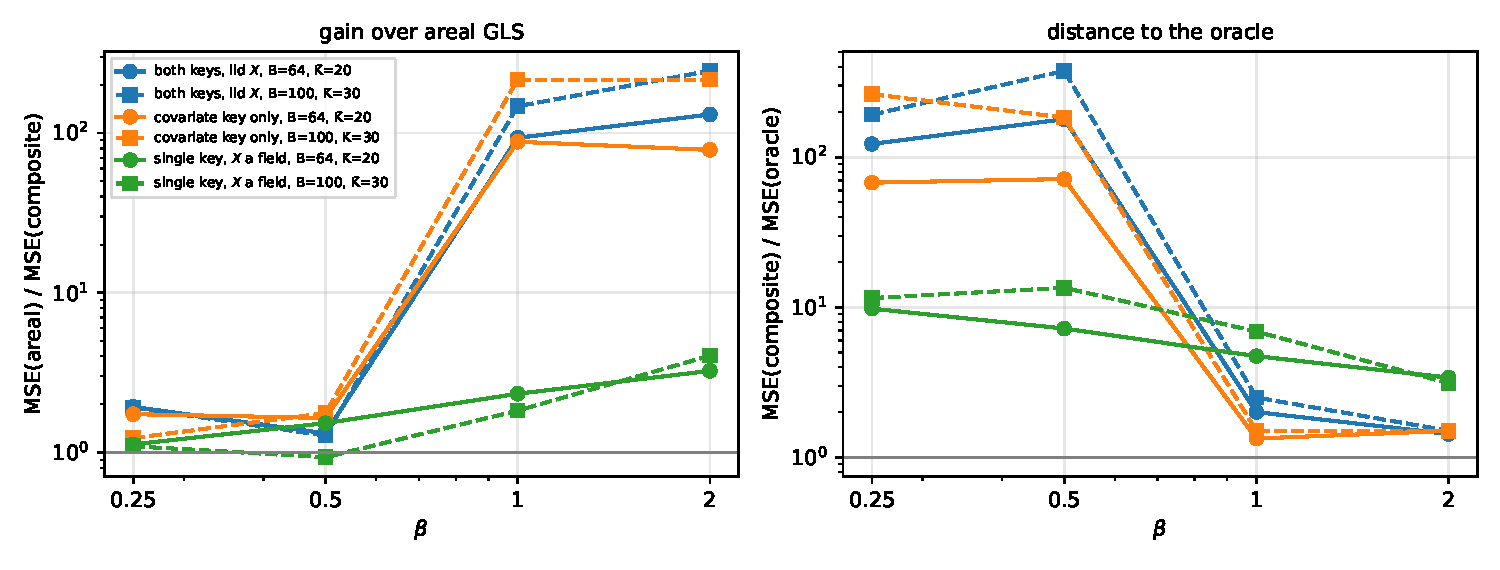
\includegraphics[width=0.8\textwidth]{Figures/beta_ratio.pdf}
\caption{Table~\ref{tab:realistic} as ratios: MSE(areal GLS)/MSE(augmented composite) (left) and MSE(augmented composite)/MSE(oracle) (right) against $\beta$, by key structure (colour) and design (solid $B=64$, $\bar K=20$; dashed $B=100$, $\bar K=30$). Figure~\ref{fig:infochecks}(a) is the per-block information version of the same curves.}
\label{fig:betaratio}
\end{figure}

\section{Spatially correlated covariates: what changes in each result}\label{sec:spatialX}

Referee~1 asks for covariates that are themselves spatially correlated. Everything above assumes $\bx_{b,i}$ i.i.d.; this section replaces that by a covariate \emph{field} and goes through the results one by one. One caveat governs the whole section: the covariate field is assumed independent of $W$, as in Assumption~\ref{ass:dgp}(iv). Under that assumption the model stays correctly specified and nothing below is a bias; what changes is information and risk. The dependent case, $g$ correlated with $W$, is the bias form of spatial confounding (Paciorek 2010; Hodges and Reich 2010), in which no estimator, oracle included, recovers $\beta$ without further assumptions; whether the free pairing makes it worse, by letting the key posterior absorb part of a smooth covariate signal into $W$, is left open (last item of the list at the end).

\begin{assumption}[Covariate field]\label{ass:field}
$\bx_{b,i}=g(s_{b,i})$ where $g=(g_1,\dots,g_d)$ is a centred Gaussian random field with separable cross-covariance $\Cov(g(s),g(s'))=C_g(s-s')\,\bSig_X$, $C_g(0)=1$, independent of $(W,\beps)$. Write $\bSig_g:=[C_g(s_i-s_j)]_{ij}$ ($n\times n$) and $v^g_{b,ij}:=2\{1-C_g(s_{b,i}-s_{b,j})\}$ for the variogram of the field at a within-block pair. Assumption~\ref{ass:dgp}(i) is the case $C_g(h)=\mathbb 1\{h=0\}$, $\bSig_g=\bI$, $v^g\equiv2$. (A covariate with an independent part is $C_g=\lambda\mathbb 1\{h=0\}+(1-\lambda)C_{g_0}$.)
\end{assumption}
Under Assumption~\ref{ass:field} the $n\times d$ matrix $\bX$ is matrix-normal with row covariance $\bSig_g$ and column covariance $\bSig_X$, so $\bX\beta\sim N_n(\bzero,\Lambda\bSig_g)$ with $\Lambda=\beta^\top\bSig_X\beta$ as before.

The field can enter in three ways, which behave differently on the risk side.
\begin{description}
\item[(S1) Exposure surface read at the released location.] The steward moves the location and reads $g$ at the released point; $X$ and $s$ are consistent and only $Y$ is mispaired with them. This is the single-key sub-case, and the case in which spatially correlated covariates are the norm (pollution, greenness, temperature).
\item[(S2) Spatially correlated attribute, both keys.] $X$ is an attribute of the record (income, age) that happens to be spatially correlated; the steward scrambles both pairings.
\item[(S3) Spatially correlated attribute, location kept.] As (S2) with $\bpi_S^{(b)}=\bI$.
\end{description}

\paragraph{Lemma~\ref{lem:sums} and Theorem~\ref{thm:sep}(a).} Step~1 of the proof uses nothing about the law of $\bX$: $\bT=\mathbf S\beta+\bU$ with $\bU$ independent of $\mathbf S$, for any keys. What is lost is the independence of the $\bS_b$ across blocks ($\Cov(\bS_b,\bS_{b'})=\bone^\top(\bSig_g)_{bb'}\bone\,\bSig_X$) and with it the invariance argument of Step~5 and the exact identity \eqref{eq:mse}. What remains: $\hat\beta_\agg$ is conditionally unbiased with $\Cov(\hat\beta_\agg\mid\mathbf S)=(\mathbf S^\top\bV^{-1}\mathbf S)^{-1}\preceq\lambda_{\max}(\bV)(\mathbf S^\top\mathbf S)^{-1}$, and under Assumption~\ref{ass:mixing} applied to the pair $(g,W)$, $B^{-1}\mathbf S^\top\mathbf S\to\bar K^2\bar\rho_g\bSig_X\succ0$ in probability, with $\bar\rho_g$ the limiting mean within-block correlation of $C_g$; so $\|\hat\beta_\agg-\beta\|=O_p(B^{-1/2})$ in all three cases, whatever the keys (this is Corollary~\ref{cor:sub}(iii)).

\paragraph{Theorem~\ref{thm:sep}(b)--(d): the floors.} The two-point argument is unchanged; only the law of the shift changes. Since $\bX\beta\sim N(\bzero,\Lambda\bSig_g)$,
\begin{equation}\label{eq:pX-g}
\Delta^X_{b,ij}=(\bx_{b,i}-\bx_{b,j})^\top\beta\sim N\big(0,\Lambda v^g_{b,ij}\big),\qquad
p^X_{b,ij}=\frac1\pi\arctan\frac{\sqrt2\,\tau}{\sqrt{\Lambda\,v^g_{b,ij}}}
\end{equation}
(Lemma~\ref{lem:arctan} with $a=\sqrt{\Lambda v^g_{b,ij}/2}/\tau$), which reduces to \eqref{eq:pX} when $v^g=2$ and tends to $\tfrac12$ for close pairs of a field without nugget: two records with nearly equal covariates are interchangeable. On the simulation design at $\Lambda=4$ ($\beta=2$, $\sigma_X=1$) the best-pair floor averages $0.35$ over blocks for an exponential covariate field with the range of $W$ and $0.47$ for a Mat\'ern-$2.5$ field, against $0.11$ for an i.i.d.\ covariate (script \texttt{sims/simD\_spatialX.py}). $p^S$ is unaffected. Part (c) holds with the pair-dependent $p^X_{b,ij}$; the refinement $p^X(1-B/n)$, which used that $p^X$ was the same for every pair, becomes $\sum_b2\sum_\ell p^X_{b,i_\ell j_\ell}/n$ over disjoint pairs. Part (d) for the covariate keys needs the differences $(\bx_{b,i_b}-\bx_{b,j_b})^\top\beta$ to be independent across blocks, which they are not; the bound becomes $\E\prod_b(1-e^X_b)$ with $e^X_b=\Phi(-|\Delta^X_{b,i_bj_b}|/(\sqrt2\tau))$, handled exactly as the location keys were in Lemma~\ref{lem:lln}, with $p_{\min}$ replaced by $\min_b p^X_{b,i_bj_b}$.

In (S2)--(S3) there is one genuinely new term. A smooth attribute's values say something about where each record sits, and the strongest adversary of Theorem~\ref{thm:sep}(b) is given the location key; so besides the regression channel it can ask whether the observed covariate values are more plausible with records $i,j$ at $(s_i,s_j)$ or at $(s_j,s_i)$. In (S1) this channel is absent, because $X$ is computed from the released location and carries no information about the true one.

\begin{proposition}[Floors with a spatially correlated attribute]\label{prop:floor-g}
Under Assumptions~\ref{ass:keys} and \ref{ass:field}, in cases (S2)--(S3), for every block $b$, pair $i\ne j$ and adversary,
\[
\Prob(\hat\bpi_X^{(b)}\ne\bpi_X^{(b)})\ \ge\ p^X_{b,ij}-\sqrt{d\,D_g(b;ij)/8},\qquad
D_g(b;ij):=\tfrac12\big[\tr\big(\bSig_g^{-1}\,(ij)\bSig_g(ij)\big)-n\big],
\]
where $(ij)$ is the $n\times n$ transposition of the two records and $p^X_{b,ij}$ is \eqref{eq:pX-g}; in (S2) the same correction applies to the location-key floor $p^S_{b,ij}$. $D_g(b;ij)$ is the Kullback--Leibler divergence between the law of one coordinate of the covariate field with and without the swap; it is the quantity $D(\bR)$ of Definition~\ref{def:constants} computed for the field $g$ and a single transposition, is zero when $s_{b,i}$ and $s_{b,j}$ are exchangeable in $\bSig_g$, and is small when $g$ has a nugget or the pair is close. In case (S1) the floors of Theorem~\ref{thm:sep} hold with \eqref{eq:pX-g} and no correction.
\end{proposition}

\paragraph{Theorem~\ref{thm:eff}.} Parts (i)--(ii) are proved conditionally on $\bX$ and hold verbatim for every realisation of $g$. Only the closed forms change: by the separable structure,
\begin{equation}\label{eq:info-g}
\mathbf I_\orc=\E[\bX^\top\bOm\bX]=\tr(\bOm\bSig_g)\,\bSig_X,\qquad \mathbf I_\agg=\E[\mathbf S^\top\bV^{-1}\mathbf S]=\tr\big(\bV^{-1}\mathbf A^\top\bSig_g\mathbf A\big)\,\bSig_X,
\end{equation}
with $\mathbf A$ the block-indicator matrix, so the oracle-to-areal gain is still the same scalar in every direction. Table~\ref{tab:spatialX} evaluates the scalars on the simulation design. A covariate as smooth as the field loses an order of magnitude of oracle information relative to an i.i.d.\ covariate of the same variance, and a very smooth covariate leaves almost nothing beyond the block sums: the gain falls from $21$ to $1.1$. This is the collinearity form of spatial confounding: the information about $\beta$ lives in the part of $X$ that is not predictable from the field, and a smooth covariate is nearly constant within a block, so its within-block contrasts, which are all that unlinking can lose, carry little. The reading is favourable to the release mechanism: for smooth covariates the analyst loses almost nothing by not knowing the pairing, the areal GLS is then nearly efficient, and the gain of the marginal likelihood is largest exactly when the covariate is rough. Part (iii) holds with Assumption~\ref{ass:mixing} imposed on the pair $(g,W)$; the composite likelihood conditions on $\bX$, so nothing else changes.

\begin{table}[t]\centering\small
\begin{tabular}{lrrr}\toprule
covariate field $g$ ($C_g(0)=1$) & $\tr(\bOm\bSig_g)$ & $\tr(\bV^{-1}\mathbf A^\top\bSig_g\mathbf A)$ & ratio\\\midrule
i.i.d. & 301.2 & 14.1 & 21.4\\
exponential, range $0.1$ & 116.1 & 23.2 & 5.0\\
exponential, range $0.5$ (as $W$) & 28.7 & 8.4 & 3.4\\
exponential, range $2$ & 7.9 & 2.8 & 2.9\\
Mat\'ern $\nu=2.5$, range $0.5$ & 2.6 & 2.4 & 1.1\\
$\tfrac12$ i.i.d.\ $+\tfrac12$ exponential, range $0.5$ & 164.9 & 11.2 & 14.7\\\bottomrule
\end{tabular}
\caption{The scalars in \eqref{eq:info-g} (oracle and areal information per unit $\bSig_X$) for covariate fields of unit variance on the simulation design ($B=49$, $K=6$, $W$ exponential with $\sigma^2=5$, range $0.5$, $\tau^2=0.5$).}
\label{tab:spatialX}
\end{table}

\paragraph{Section~\ref{sec:full}.} Lemma~\ref{lem:decay} and Proposition~\ref{prop:order} concern $\bOm$ and the block sums; the proposition's bounds become $\{\lambda_{\min}(\bSig_g)K_{\min}B/(\bar K(\tau^2+M))\}\bSig_X\preceq\mathbf I_\agg$ and $\mathbf I_\orc\preceq\{\lambda_{\max}(\bSig_g)\bar KB/\tau^2\}\bSig_X$, where $\lambda_{\max}(\bSig_g)$ is bounded under increasing domain by the argument of Lemma~\ref{lem:decay}(i) applied to $C_g$ but $\lambda_{\min}(\bSig_g)$ can be small for a smooth field without nugget; Theorem~\ref{thm:onestep} is conditional on (C1)--(C2) and does not involve the law of $\bX$.

\paragraph{Theorem~\ref{thm:common}.} Case~2 of the proof (relative alignment right, location key wrong) does not involve $\bX$ and is unchanged: the location key is recovered from the covariance shift $\delta_{\mathrm{cov}}$ alone. Case~1 uses the law of $\bX\beta$ through the quadratic forms of Part~B. With $\bX\beta=\sqrt\Lambda\,\bSig_g^{1/2}\bm\xi$, $\bm\xi\sim N(\bzero,\bI_n)$, each form $\bm\xi^\top\mathbf G_\ast\bm\xi$ becomes $\bm\xi^\top\bSig_g^{1/2}\mathbf G_\ast\bSig_g^{1/2}\bm\xi$, with trace $\tr(\mathbf G_\ast\bSig_g)$. For the signal term this is $\tr\{(\mathbf Q-\bI)^\top\bOm(\mathbf Q-\bI)\bSig_g\}=\tr\{\bOm\,\Cov((\mathbf Q-\bI)\bX\beta)\}/\Lambda$, the precision-weighted variance of the covariate differences across the moved pairs, which for an i.i.d.\ covariate is at least $2h_{12}/\tau_c^2$ and for a covariate field is of the order of $h_{12}$ times a within-block variogram of $g$ divided by $\tau_c^2$: it vanishes as $g$ becomes smooth, consistently with the floors \eqref{eq:pX-g}. Two further changes make a restatement with explicit constants not worth having: the Hanson--Wright norms acquire the factor $\lambda_{\max}(\bSig_g)$, and the angle-lemma step needs $\|\bm a\|/\|\bm b\|$ bounded below, which for a covariate field costs $\kappa(\bSig_g)^{-1/2}$ because $\tr(\mathbf Q^\top\bOm\mathbf Q\bSig_g)$ and $\tr(\bOm\bSig_g)$ are no longer equal. The qualitative content survives: under a common key the covariate channel recovers the key at rate $e^{-cB}$ with a signal-to-noise ratio built from the within-block variogram of $g$ instead of $\Lambda$, and the location channel is untouched.

\paragraph{What this says for the paper.} With independence of $g$ and $W$, spatially correlated covariates can go into the main text at the cost of Assumption~\ref{ass:field}, \eqref{eq:pX-g}, \eqref{eq:info-g} with Table~\ref{tab:spatialX}, and Proposition~\ref{prop:floor-g}: they cost information (a smooth covariate is nearly constant within a block, so unlinking is almost free for the analyst) and they raise the re-linking floors, with one extra channel when the location is known; the separation and the efficiency ordering are untouched, and the exposure-surface case (S1), the one that occurs in the applications, has the clean version of every statement. The simulation design should then include $X$ drawn from a Gaussian field with the same and with a shorter range than $W$, and with an i.i.d.\ component, in the three cases.

\section*{What remains to be done}
\begin{enumerate}
\item Verify conditions (C1)--(C2) of Theorem~\ref{thm:onestep} for the full marginal likelihood (Remark~\ref{rem:obstacle}): a decay-of-correlations argument for the key posterior. This is the one open theoretical item; everything else in the efficiency story is proved for the composite likelihood and checked numerically.
\item Put the estimator of Section~\ref{sec:realistic} into the code (per-block key sampler, damped Newton from the areal fit, covariance parameters from the areal stage), check the variational relaxation against the chain and, at $K\le5$, against enumeration, and add the empirical per-record re-linking rate of the two-key adversary at realistic $K$ next to the floors.
\item Remove the factor $K!$ (absorbed in $K^{K+2}$) from Theorem~\ref{thm:common} by using the decay of the covariance term in $k_2$, as in the submitted proof.
\item The dependent case $g\not\perp W$ (Section~\ref{sec:spatialX}): whether the free pairing lets the key posterior absorb part of a smooth covariate signal into $W$, to be checked numerically before anything is claimed; and simulations with spatially correlated covariates in the three cases (S1)--(S3) against the floors \eqref{eq:pX-g} and Proposition~\ref{prop:floor-g}.
\end{enumerate}

\appendix

\section{Proofs for Sections~\ref{sec:sep}--\ref{sec:subresults}}\label{app:sep}

\begin{proof}[Proof of Lemma~\ref{lem:sums}]
\emph{Step 1: the sums.} Fix a block $b$ and any permutation matrix $\bpi$ of size $K_b$. Each column of $\bpi$ contains exactly one $1$, so $\bone^\top\bpi=\bone^\top$. Multiplying \eqref{eq:model} on the left by $\bone^\top$,
\[
T_b=\bone^\top\bY_b=\bone^\top\bpi_X^{(b)}\bX_b\,\beta+\bone^\top\bpi_S^{(b)}\bW_b+\bone^\top\beps_b=\bone^\top\bX_b\,\beta+\bone^\top\bW_b+\bone^\top\beps_b=\bS_b^\top\beta+U_b,
\]
with $\bS_b=\bX_b^\top\bone$ and $U_b:=\bone^\top\bW_b+\bone^\top\beps_b$. The keys have disappeared, so the identity holds whatever they are and however they were chosen.

\emph{Step 2: distributions.} By Assumption~\ref{ass:dgp}(i), $\bS_b=\sum_{i=1}^{K_b}\bx_{b,i}$ is a sum of $K_b$ independent $N_d(\bzero,\bSig_X)$ vectors, so $\bS_b\sim N_d(\bzero,K_b\bSig_X)$, and different blocks involve disjoint sets of covariate vectors, so the $\bS_b$ are independent. By (ii)--(iii), $\bU$ is a linear image of the Gaussian vector $(\bW,\beps)$, hence Gaussian with mean zero and
\begin{align*}
\Cov(U_b,U_{b'})&=\Cov(\bone^\top\bW_b,\bone^\top\bW_{b'})+\Cov(\bone^\top\beps_b,\bone^\top\beps_{b'})\\
&=\bone^\top(\bSig_W)_{bb'}\bone+\tau^2K_b\mathbb 1\{b=b'\}=\bone^\top\bSig^\ast_{bb'}\bone=V_{bb'},
\end{align*}
using that $\beps$ has covariance $\tau^2\bI_n$ so $\bone^\top\Cov(\beps_b,\beps_{b'})\bone=\tau^2\bone^\top\bI\bone\,\mathbb 1\{b=b'\}=\tau^2K_b\mathbb 1\{b=b'\}$. By (iv), $\bU$ is independent of $\mathbf S$.

\emph{Step 3: the estimator error.} Write $\bS_b=\sqrt{K_b}\,\bSig_X^{1/2}\bz_b$ with $\bz_b$ i.i.d.\ $N_d(\bzero,\bI_d)$ (Step~2), let $\mathbf Z$ be the $B\times d$ matrix with rows $\bz_b^\top$, and $\tilde U_b:=U_b/\sqrt{K_b}$, so that $\tilde\bU\sim N_B(\bzero,\tilde\bV)$ with $\tilde V_{bb'}=V_{bb'}/\sqrt{K_bK_{b'}}$, i.e.\ $\tilde\bV=\bD^{-1/2}\bV\bD^{-1/2}$, independent of $\mathbf Z$. Then $K_b^{-1}\bS_b\bS_b^\top=\bSig_X^{1/2}\bz_b\bz_b^\top\bSig_X^{1/2}$, so $\sum_bK_b^{-1}\bS_b\bS_b^\top=\bSig_X^{1/2}\mathbf Z^\top\mathbf Z\bSig_X^{1/2}$, and $K_b^{-1}\bS_bT_b=K_b^{-1}\bS_b\bS_b^\top\beta+K_b^{-1}\bS_bU_b=K_b^{-1}\bS_b\bS_b^\top\beta+\bSig_X^{1/2}\bz_b\tilde U_b$. Substituting into the definition of $\tilde\beta$,
\[
\tilde\beta=\big(\bSig_X^{1/2}\mathbf Z^\top\mathbf Z\bSig_X^{1/2}\big)^{-1}\Big(\bSig_X^{1/2}\mathbf Z^\top\mathbf Z\bSig_X^{1/2}\beta+\bSig_X^{1/2}\mathbf Z^\top\tilde\bU\Big)=\beta+\bSig_X^{-1/2}(\mathbf Z^\top\mathbf Z)^{-1}\mathbf Z^\top\tilde\bU,
\]
using $(\bSig_X^{1/2}\mathbf Z^\top\mathbf Z\bSig_X^{1/2})^{-1}=\bSig_X^{-1/2}(\mathbf Z^\top\mathbf Z)^{-1}\bSig_X^{-1/2}$. For $d=1$ this is $\tilde\beta-\beta=\sigma_X^{-1}\bZ^\top\tilde\bU/\|\bZ\|^2$.

\emph{Step 4: conditional second moment.} Conditionally on $\mathbf Z$, $\mathbf Z^\top\tilde\bU$ is a linear image of the centred Gaussian vector $\tilde\bU$ with fixed coefficients, so $\E[\mathbf Z^\top\tilde\bU\mid\mathbf Z]=\bzero$ and $\Cov(\mathbf Z^\top\tilde\bU\mid\mathbf Z)=\mathbf Z^\top\tilde\bV\mathbf Z$. Hence $\E[\tilde\beta\mid\mathbf Z]=\beta$ and
\[
\E\big[(\tilde\beta-\beta)(\tilde\beta-\beta)^\top\mid\mathbf Z\big]=\bSig_X^{-1/2}(\mathbf Z^\top\mathbf Z)^{-1}\mathbf Z^\top\tilde\bV\mathbf Z(\mathbf Z^\top\mathbf Z)^{-1}\bSig_X^{-1/2}.
\]

\emph{Step 5: the expectation over $\mathbf Z$.} Let $\mathbf R:=(\mathbf Z^\top\mathbf Z)^{1/2}$ ($d\times d$, invertible almost surely since $B\ge d$) and $\mathbf Q:=\mathbf Z\mathbf R^{-1}$, a $B\times d$ matrix with orthonormal columns ($\mathbf Q^\top\mathbf Q=\mathbf R^{-1}\mathbf Z^\top\mathbf Z\mathbf R^{-1}=\bI_d$). For $d=1$, $\mathbf R=\|\bZ\|$ and $\mathbf Q=\bZ/\|\bZ\|$. The law of $\mathbf Z$ is invariant under $\mathbf Z\mapsto\mathbf O\mathbf Z$ for every $B\times B$ orthogonal $\mathbf O$, which maps $(\mathbf Q,\mathbf R)\mapsto(\mathbf O\mathbf Q,\mathbf R)$; hence $\mathbf Q$ is uniformly distributed on the Stiefel manifold of $B\times d$ orthonormal frames and is independent of $\mathbf R$ (Muirhead 1982, Ch.~3; for $d=1$, the direction of a standard Gaussian vector is uniform on the sphere and independent of its length). Then
\[
(\mathbf Z^\top\mathbf Z)^{-1}\mathbf Z^\top\tilde\bV\mathbf Z(\mathbf Z^\top\mathbf Z)^{-1}=\mathbf R^{-1}\mathbf Q^\top\tilde\bV\mathbf Q\mathbf R^{-1},\qquad
\E\big[\mathbf R^{-1}\mathbf Q^\top\tilde\bV\mathbf Q\mathbf R^{-1}\big]=\E\big[\mathbf R^{-1}\,\E[\mathbf Q^\top\tilde\bV\mathbf Q]\,\mathbf R^{-1}\big]
\]
by independence. Now $\E[\mathbf Q^\top\tilde\bV\mathbf Q]=(\tr\tilde\bV/B)\,\bI_d$: the law of $\mathbf Q$ is also invariant under $\mathbf Q\mapsto\mathbf Q\mathbf P$ for $d\times d$ orthogonal $\mathbf P$ (this is $\mathbf Z\mapsto\mathbf Z\mathbf P$, which preserves the law of $\mathbf Z$ and maps $\mathbf R\mapsto\mathbf P^\top\mathbf R\mathbf P$), so $\E[\mathbf Q^\top\tilde\bV\mathbf Q]=\mathbf P^\top\E[\mathbf Q^\top\tilde\bV\mathbf Q]\mathbf P$ for all $\mathbf P$, which forces a multiple $c\,\bI_d$; its trace is $dc=\E\tr(\tilde\bV\mathbf Q\mathbf Q^\top)=\tr(\tilde\bV\,\E[\mathbf Q\mathbf Q^\top])$, and $\E[\mathbf Q\mathbf Q^\top]$ is invariant under conjugation by $B\times B$ orthogonal matrices, hence $c'\bI_B$ with $Bc'=\E\tr(\mathbf Q\mathbf Q^\top)=\E\tr(\mathbf Q^\top\mathbf Q)=d$; so $dc=(d/B)\tr\tilde\bV$. Finally $\mathbf R^{-2}=(\mathbf Z^\top\mathbf Z)^{-1}$, the inverse of a $W_d(B,\bI_d)$ Wishart matrix, has mean $\bI_d/(B-d-1)$ for $B\ge d+2$ (Muirhead 1982, Ch.~3); for $d=1$ this is $\E[1/\chi^2_B]=\int_0^\infty x^{-1}\frac{x^{B/2-1}e^{-x/2}}{2^{B/2}\Gamma(B/2)}dx=\frac{\Gamma(B/2-1)}{2\Gamma(B/2)}=\frac1{B-2}$. Combining,
\[
\E(\tilde\beta-\beta)(\tilde\beta-\beta)^\top=\bSig_X^{-1/2}\,\frac{\tr\tilde\bV}{B}\,\E[\mathbf R^{-2}]\,\bSig_X^{-1/2}=\frac{\tr(\bD^{-1/2}\bV\bD^{-1/2})}{B(B-d-1)}\,\bSig_X^{-1},
\]
which is the identity in \eqref{eq:mse}.

\emph{Step 6: the bound.} $\tr(\tilde\bV)=\sum_b\tilde V_{bb}=\sum_bV_{bb}/K_b$ and $V_{bb}=\bone^\top(\bSig_W)_{bb}\bone+K_b\tau^2$. By Cauchy--Schwarz and Assumption~\ref{ass:dgp}(ii), $|(\bSig_W)_{ij}|\le\sqrt{(\bSig_W)_{ii}(\bSig_W)_{jj}}\le\sigma^2$, so $\bone^\top(\bSig_W)_{bb}\bone=\sum_{i,j\le K_b}(\bSig_W)_{ij}\le K_b^2\sigma^2$. Therefore $V_{bb}/K_b\le K_b\sigma^2+\tau^2\le\bar K\sigma^2+\tau^2$ and $\tr(\tilde\bV)\le B(\bar K\sigma^2+\tau^2)$; inserting this into the identity gives the bound in \eqref{eq:mse}, in the Loewner order because $\bSig_X^{-1}\succ0$.

\emph{Step 7: the GLS.} Conditionally on $\mathbf S$, $\bT=\mathbf S\beta+\bU$ is a linear model with known error covariance $\bV$ (Step 2). $\hat\beta_\agg$ is its generalised least-squares estimator, and $\tilde\beta$ is a linear function of $\bT$ with $\E[\tilde\beta\mid\mathbf S]=\beta$ (Step 4). By the Gauss--Markov theorem (in its matrix form: the GLS covariance is smallest in the Loewner order among linear unbiased estimators), $\Cov(\hat\beta_\agg\mid\mathbf S)\preceq\Cov(\tilde\beta\mid\mathbf S)$. Both are conditionally unbiased, so their conditional mean-squared-error matrices equal their conditional covariances, and taking expectations over $\mathbf S$ preserves the order.
\end{proof}

\begin{proof}[Proof of Lemma~\ref{lem:twopoint}]
With equal prior weights, the Bayes test with respect to the $0$--$1$ loss decides $H=1$ when the likelihood ratio exceeds one, i.e.\ when
\[
\log\frac{\phi(\bY;\bmu_1,\tau^2\bI)}{\phi(\bY;\bmu_0,\tau^2\bI)}=\frac{-\|\bY-\bmu_1\|^2+\|\bY-\bmu_0\|^2}{2\tau^2}=\frac{(\bmu_1-\bmu_0)^\top\big(\bY-\tfrac12(\bmu_0+\bmu_1)\big)}{\tau^2}>0,
\]
where the middle equality expands the two squared norms and cancels $\|\bY\|^2$. Let $\bm d:=\bmu_1-\bmu_0$ and $L:=\bm d^\top(\bY-\tfrac12(\bmu_0+\bmu_1))$. Under $H=0$, $\bY=\bmu_0+\tau\bm\eta$ with $\bm\eta\sim N(\bzero,\bI)$, so $\bY-\tfrac12(\bmu_0+\bmu_1)=-\tfrac12\bm d+\tau\bm\eta$ and $L=-\tfrac12\|\bm d\|^2+\tau\bm d^\top\bm\eta\sim N(-\tfrac12\|\bm d\|^2,\tau^2\|\bm d\|^2)$. The type-I error is therefore
\[
\Prob_0(L>0)=\Prob\Big(N(0,1)>\frac{\tfrac12\|\bm d\|^2}{\tau\|\bm d\|}\Big)=1-\Phi\Big(\frac{\|\bm d\|}{2\tau}\Big)=\Phi\Big(-\frac{\|\bm d\|}{2\tau}\Big).
\]
Under $H=1$, $L=+\tfrac12\|\bm d\|^2+\tau\bm d^\top\bm\eta$ and the type-II error $\Prob_1(L\le0)$ is the same number. The Bayes error is the average of the two, $\Phi(-\|\bm d\|/(2\tau))$, and by the definition of the Bayes test no other test has a smaller prior-averaged error.
\end{proof}

\begin{proof}[Proof of Lemma~\ref{lem:arctan}]
Let $N\sim N(0,1)$ be independent of $Z$. Since $\Phi(-a|z|)=\Prob(N<-a|z|)$ for each fixed $z$, $\E\,\Phi(-a|Z|)=\Prob(N<-a|Z|)$. Split according to the sign of $Z$:
\[
\Prob(N<-a|Z|)=\Prob(N<-aZ,\,Z>0)+\Prob(N<aZ,\,Z<0)=2\,\Prob(N<-aZ,\,Z>0),
\]
the second term equalling the first by the symmetry $Z\mapsto-Z$. In the $(n,z)$-plane the pair $(N,Z)$ has the rotation-invariant standard bivariate normal law, so the probability of any wedge with vertex at the origin is its opening angle divided by $2\pi$. The set $\{z>0,\ n<-az\}$ is the wedge bounded by the negative $n$-axis (angle $\pi$ from the positive $n$-axis) and the ray $\{(n,z)=t(-a,1):t>0\}$, whose angle from the positive $n$-axis is $\pi-\arctan(1/a)$; its opening is therefore $\arctan(1/a)$. Hence $2\Prob(N<-aZ,Z>0)=2\cdot\arctan(1/a)/(2\pi)=\pi^{-1}\arctan(1/a)$.
\end{proof}

\begin{proof}[Proof of Theorem~\ref{thm:sep}]
(a) is Lemma~\ref{lem:sums}.

\emph{Notation for permutations.} A permutation of block $b$ is a bijection $\sigma$ of $\{1,\dots,K_b\}$; its matrix $\bsigma$ is defined by $\bsigma\bm e_i=\bm e_{\sigma(i)}$, so that $(\bsigma\bm x)_{\sigma(i)}=x_i$: the record in position $i$ is moved to position $\sigma(i)$. Products are matrix products, so $\bsigma\bm\rho$ moves records first by $\rho$ and then by $\sigma$, and $\bsigma^{-1}=\bsigma^\top$. For $i\ne j$, $(ij)$ denotes the \emph{transposition} that exchanges $i$ and $j$ and fixes every other index; its matrix is $\bI-(\bm e_i-\bm e_j)(\bm e_i-\bm e_j)^\top$, it is its own inverse, and $(ij)\ne\bI$ because $i\ne j$. Thus $\bsigma(ij)$ is the permutation that agrees with $\sigma$ except that it sends $i$ to $\sigma(j)$ and $j$ to $\sigma(i)$: the records $i$ and $j$ have their destinations exchanged.

\emph{(b), covariate key.} Fix $b$ and $i\ne j$. We bound the error of the strongest adversary described before the theorem; a weaker adversary can only do worse. So condition on $\bX$, on the field values $\bW^\rel:=(\bW_{b'})_{b'}$ at the released locations, and on every key except $\bpi_X^{(b)}$, and treat these as known.

\emph{Step 1: only block $b$ matters.} The field is dependent across blocks, and unconditionally $\bY_{b'}$ does carry information about $\bW_b$ and hence about $\bY_b$. But we have conditioned on the whole vector $\bW^\rel$, so $\bW_b$ and $\bW_{b'}$ are now fixed numbers, not random variables, and the cross-block dependence has been handed to the adversary in its entirety; conditioning on more can only reduce the Bayes error, so a bound proved under this conditioning holds for every adversary. Given the conditioning, $\bY_{b'}=\bpi_X^{(b')}\bX_{b'}\beta+\bpi_S^{(b')}\bW_{b'}+\beps_{b'}$ for $b'\ne b$ is a known vector plus $\beps_{b'}$, and $\bY_b=\bpi_X^{(b)}\bX_b\beta+\bpi_S^{(b)}\bW_b+\beps_b$ is a function of $(\bpi_X^{(b)},\beps_b)$ only. The noise vectors $\beps_1,\dots,\beps_B$ are mutually independent, and independent of $(\bX,\bW)$ and of the keys (Assumptions~\ref{ass:dgp}(iii)--(iv) and \ref{ass:keys}), so the random ingredients of $(\bY_{b'})_{b'\ne b}$, namely $(\beps_{b'})_{b'\ne b}$, are independent of the random ingredients of $(\bY_b,\bpi_X^{(b)})$, namely $(\beps_b,\bpi_X^{(b)})$. Hence $(\bY_{b'})_{b'\ne b}$ is conditionally independent of $(\bY_b,\bpi_X^{(b)})$ and carries no information about $\bpi_X^{(b)}$. It follows that the Bayes error for $\bpi_X^{(b)}$ is the same whether or not these vectors are observed, and we may work with $\bY_b$ alone, whose conditional law is
\[
\bY_b\ \big|\ \bpi_X^{(b)}=\bsigma\ \sim\ N\big(\bsigma\bX_b\beta+\bpi_S^{(b)}\bW_b,\ \tau^2\bI_{K_b}\big),\qquad\bsigma\text{ uniform on }\calS_{K_b}.
\]

\emph{Step 2: reduce to two hypotheses.} The map $\bsigma\mapsto\bsigma(ij)$ sends $\calS_{K_b}$ to itself; applying it twice gives $\bsigma(ij)(ij)=\bsigma$, so it is an involution; and it has no fixed point, since $\bsigma(ij)=\bsigma$ would give, after multiplying on the left by $\bsigma^{-1}$, $(ij)=\bI$, which is false. An involution without fixed points pairs up the elements of the set, so it partitions $\calS_{K_b}$ into $K_b!/2$ pairs $\{\bsigma,\bsigma(ij)\}$. Suppose the adversary is additionally told which pair contains the true key. Because the prior is uniform on $\calS_{K_b}$, the conditional prior given the pair puts mass $\frac12$ on each of its two elements. Extra information cannot increase the Bayes error, so the Bayes error of the original problem is at least the Bayes error of this two-point problem.

\emph{Step 3: the two means.} Under the two hypotheses the mean of $\bY_b$ is $\bmu_0=\bsigma\bX_b\beta+\bpi_S^{(b)}\bW_b$ and $\bmu_1=\bsigma(ij)\bX_b\beta+\bpi_S^{(b)}\bW_b$. The vector $\bX_b\beta$ has entries $\bx_{b,k}^\top\beta$, and $(ij)\bX_b\beta$ is that vector with its $i$-th and $j$-th entries exchanged, so $(ij)\bX_b\beta-\bX_b\beta=(\bx_{b,j}-\bx_{b,i})^\top\beta\,\bm e_i+(\bx_{b,i}-\bx_{b,j})^\top\beta\,\bm e_j=(\bx_{b,j}-\bx_{b,i})^\top\beta\,(\bm e_i-\bm e_j)$. Applying $\bsigma$ (which maps $\bm e_i\mapsto\bm e_{\sigma(i)}$),
\begin{gather*}
\bmu_1-\bmu_0=\bsigma\{(ij)\bX_b\beta-\bX_b\beta\}=(\bx_{b,j}-\bx_{b,i})^\top\beta\,(\bm e_{\sigma(i)}-\bm e_{\sigma(j)}),\\
\|\bmu_1-\bmu_0\|^2=\{(\bx_{b,j}-\bx_{b,i})^\top\beta\}^2\cdot2=2(\Delta^X_{b,ij})^2 .
\end{gather*}

\emph{Step 4: the error bound.} By Lemma~\ref{lem:twopoint} the two-point Bayes error given $(\bX,\bW^\rel)$ is $\Phi(-\|\bmu_1-\bmu_0\|/(2\tau))=\Phi(-\sqrt2|\Delta^X_{b,ij}|/(2\tau))=\Phi(-|\Delta^X_{b,ij}|/(\sqrt2\tau))$. By Step~2 this is a lower bound on the conditional error of every estimator of $\bpi_X^{(b)}$. Taking the expectation over $(\bX,\bW^\rel)$,
\[
\Prob(\hat\bpi_X^{(b)}\ne\bpi_X^{(b)})\ \ge\ \E\,\Phi\Big(-\frac{|\Delta^X_{b,ij}|}{\sqrt2\tau}\Big)=p^X_{b,ij},
\]
and the closed form is \eqref{eq:pX}.

\emph{(b), location key.} Identical, with $\bpi_X^{(b)}$ given and $\bpi_S^{(b)}=\bsigma$ unknown. Now $\bmu_1-\bmu_0=\bsigma\{(ij)\bW_b-\bW_b\}=(W(s_{b,j})-W(s_{b,i}))(\bm e_{\sigma(i)}-\bm e_{\sigma(j)})$, of squared norm $2(\Delta^S_{b,ij})^2$, and the same steps give the bound $p^S_{b,ij}$ with closed form \eqref{eq:pS}. Note that $\beta$ does not appear anywhere.

\emph{(b), single key.} With $\bpi_X^{(b)}=\bpi_S^{(b)}=\bsigma$, $\bmu_1-\bmu_0=\bsigma\{(ij)(\bX_b\beta+\bW_b)-(\bX_b\beta+\bW_b)\}=\big((\bx_{b,j}-\bx_{b,i})^\top\beta+W(s_{b,j})-W(s_{b,i})\big)(\bm e_{\sigma(i)}-\bm e_{\sigma(j)})$, of squared norm $2(\Delta^{XS}_{b,ij})^2$.

\emph{(c).} Apply (b) to each block $b$ with its best pair to get $\Prob(\text{block $b$ wrong})\ge\max_{i\ne j}p_{b,ij}\ge p_0$; the expected number of wrong blocks is $\sum_b\Prob(\text{block $b$ wrong})\ge Bp_0$ by linearity of expectation. If the key of block $b$ is wrong, the estimated and true permutations differ in at least two positions (two permutations that agree in all but one position agree everywhere), so at least two records of the block are misplaced; hence the expected number of misplaced records is at least $2Bp_0$, i.e.\ a fraction at least $2Bp_0/n\ge2p_0/\bar K$.

For the refined statement fix block $b$ and $m$ pairs $(i_\ell,j_\ell)$, $\ell=1,\dots,m$, no two of which share an index. For $\omega\in\{0,1\}^m$ let $\bm t_\omega:=\prod_{\ell:\,\omega_\ell=1}(i_\ell j_\ell)$ be the permutation that exchanges $i_\ell$ with $j_\ell$ for every $\ell$ with $\omega_\ell=1$ and fixes every other index; because the pairs are disjoint, the factors act on disjoint sets of indices, so their order is immaterial, $\bm t_\omega\bm t_{\omega'}=\bm t_{\omega\oplus\omega'}$ with $\oplus$ the coordinatewise sum modulo 2, and $\bm t_\omega^{-1}=\bm t_\omega$. Call $\bsigma,\bsigma'\in\calS_{K_b}$ equivalent if $\bsigma'=\bsigma\bm t_\omega$ for some $\omega$. This is an equivalence relation (reflexive with $\omega=\bzero$; symmetric because $\bsigma=\bsigma'\bm t_\omega^{-1}=\bsigma'\bm t_\omega$; transitive by the product rule), so $\calS_{K_b}$ is partitioned into its classes $C(\bsigma):=\{\bsigma\bm t_\omega:\omega\in\{0,1\}^m\}$, and each class has exactly $2^m$ elements, since $\bsigma\bm t_\omega=\bsigma\bm t_{\omega'}$ forces $\bm t_\omega=\bm t_{\omega'}$ and hence $\omega=\omega'$. (In the language of group theory the $\bm t_\omega$ form a subgroup and the classes are its cosets; only the three facts just listed are used.) Reveal to the adversary the class containing the true key, say $C(\bsigma)$. Because the prior is uniform on $\calS_{K_b}$ and all classes have the same size, the conditional prior is uniform on $C(\bsigma)$; the unknown is now the vector $\omega$, uniform on $\{0,1\}^m$, and the true key is $\bsigma\bm t_\omega$. Under $\bsigma\bm t_\omega$ the record in position $i_\ell$ is moved to $\sigma(i_\ell)$ if $\omega_\ell=0$ and to $\sigma(j_\ell)$ if $\omega_\ell=1$, and the record in position $j_\ell$ goes to the other of the two destinations; so whenever $\hat\omega_\ell\ne\omega_\ell$, both records $i_\ell$ and $j_\ell$ are placed at wrong positions. Fix $\ell$ and consider an adversary that is additionally told $\omega_{\ell'}$ for every $\ell'\ne\ell$. It faces a two-point problem between the two keys $\bsigma\bm t_\omega$ with $\omega_\ell=0$ and with $\omega_\ell=1$, which differ by the single transposition $(i_\ell j_\ell)$; exactly as in Step~3, the two means of $\bY_b$ then differ by $\Delta_{b,i_\ell j_\ell}$ in one coordinate and $-\Delta_{b,i_\ell j_\ell}$ in another, and Lemma~\ref{lem:twopoint} gives $\Prob(\hat\omega_\ell\ne\omega_\ell)\ge\E\Phi(-|\Delta_{b,i_\ell j_\ell}|/(\sqrt2\tau))=p_{b,i_\ell j_\ell}$ for this adversary, hence for any adversary. Summing over $\ell$ and counting two records per wrong coordinate gives $\E[\#\text{misplaced records in block }b]\ge2\sum_\ell p_{b,i_\ell j_\ell}$. For the covariate key, $p^X_{b,i_\ell j_\ell}=p^X$ for every pair by \eqref{eq:pX}; taking $m=\lfloor K_b/2\rfloor$ disjoint pairs gives at least $2\lfloor K_b/2\rfloor p^X\ge(K_b-1)p^X$ misplaced records in block $b$ in expectation, and summing over blocks, at least $(n-B)p^X$ in all, i.e.\ a fraction $p^X(1-B/n)$; finally $B/n\le1/K_{\min}$.

\emph{(d).} Condition on $(\bX,\bW^\rel)$ and reveal, for every block, the pair $\{\bsigma_b,\bsigma_b(i_bj_b)\}$ containing its true covariate key. The unknown is then the vector $(H_1,\dots,H_B)\in\{0,1\}^B$ of pair indicators, with a product-uniform prior. Given $(\bX,\bW^\rel)$ and the keys, the $\bY_b$ are independent (they involve disjoint $\beps_b$'s), so the joint likelihood is $\prod_bf_b(\bY_b\mid H_b)$ and the posterior of $(H_1,\dots,H_B)$ factorises into $\prod_b\Prob(H_b\mid\bY_b)$. For the $0$--$1$ loss on the whole vector the Bayes rule is the joint posterior mode, which for a product posterior is the vector of marginal modes; its success probability is $\prod_b\{1-e_b\}$ where $e_b$ is the per-block two-point Bayes error, $e_b=\Phi(-|\Delta^X_{b,i_bj_b}|/(\sqrt2\tau))$ by Lemma~\ref{lem:twopoint}. No rule can have a larger success probability under this prior, and the original adversary has less information, so
\[
\Prob\big(\text{all covariate keys correct}\ \big|\ \bX,\bW^\rel\big)\le\prod_{b=1}^B\Big\{1-\Phi\Big(-\frac{|\Delta^X_{b,i_bj_b}|}{\sqrt2\tau}\Big)\Big\}.
\]
Each factor depends on $(\bX,\bW^\rel)$ only through $(\bx_{b,i_b}-\bx_{b,j_b})^\top\beta$, and these differences are independent across blocks; taking the expectation, the expectation of the product is the product of the expectations, $\prod_b(1-p^X_{b,i_bj_b})=(1-p^X)^B$ by \eqref{eq:pX}.

For the location keys the same argument gives $\Prob(\text{all correct}\mid\bX,\bW^\rel)\le\prod_b(1-e^S_b)$ with $e^S_b=\Phi(-|\Delta^S_{b,i_bj_b}|/(\sqrt2\tau))$; here the factors depend on $\bW$ and are not independent across blocks, so we only use $\prod_b(1-e^S_b)\le\prod_b\exp(-e^S_b)=\exp(-\sum_be^S_b)$ (from $1-x\le e^{-x}$). Lemma~\ref{lem:lln} below bounds the expectation of the right-hand side.
\end{proof}

\begin{lemma}[Location keys: the sum of the per-block errors]\label{lem:lln}
Let Assumption~\ref{ass:dgp} and Assumption~\ref{ass:mixing}(ii) hold, let $e^S_b:=\Phi(-|\Delta^S_{b,i_bj_b}|/(\sqrt2\tau))$ for one pair $(i_b,j_b)$ per block, and let $p_{\min}:=\pi^{-1}\arctan(\tau/(\sqrt2\sigma))$. Then (i) $\E e^S_b\ge p_{\min}$ for every $b$; (ii) $\Var(\sum_be^S_b)\le BA_\alpha$; (iii) $\E\prod_b(1-e^S_b)\le e^{-Bp_{\min}/2}+4A_\alpha/(Bp_{\min}^2)$.
\end{lemma}
\begin{proof}
(i) $\Delta^S_{b,i_bj_b}=W(s_{b,j_b})-W(s_{b,i_b})\sim N(0,v_b)$ with $v_b=(\bSig_W)_{ii}+(\bSig_W)_{jj}-2(\bSig_W)_{ij}\le\sigma^2+\sigma^2+2\sigma^2=4\sigma^2$, using $|(\bSig_W)_{ij}|\le\sigma^2$ (Cauchy--Schwarz and Assumption~\ref{ass:dgp}(ii)). By \eqref{eq:pS}, $\E e^S_b=\pi^{-1}\arctan(\sqrt2\tau/\sqrt{v_b})$, and since $\arctan$ is increasing and $\sqrt{v_b}\le2\sigma$, this is at least $\pi^{-1}\arctan(\sqrt2\tau/(2\sigma))=p_{\min}$.

(ii) Each $e^S_b$ is a measurable function of $\bW_b$ with values in $[0,\tfrac12]$ (the argument of $\Phi$ is nonpositive), so $\Var(e^S_b)\le\|e^S_b\|_\infty^2\le\tfrac14$. For $b\ne b'$ the covariance inequality for strongly mixing variables (Ibragimov 1962; Doukhan 1994, \S1.2.2, Theorem 3) gives
\[
|\Cov(e^S_b,e^S_{b'})|\le4\|e^S_b\|_\infty\|e^S_{b'}\|_\infty\,\alpha(\sigma(\bW_b),\sigma(\bW_{b'}))\le4\cdot\tfrac12\cdot\tfrac12\,\bar\alpha(d(b,b'))=\bar\alpha(d(b,b')).
\]
Therefore
\[
\begin{aligned}
\Var\Big(\sum_be^S_b\Big)&=\sum_b\Var(e^S_b)+\sum_b\sum_{b'\ne b}\Cov(e^S_b,e^S_{b'})\\
&\le\frac B4+\sum_b\sum_{b'\ne b}\bar\alpha(d(b,b'))\le B\Big(\frac14+\sup_b\sum_{b'\ne b}\bar\alpha(d(b,b'))\Big)=BA_\alpha .
\end{aligned}
\]

(iii) From $1-x\le e^{-x}$, $\prod_b(1-e^S_b)\le\exp(-\sum_be^S_b)$. Let $E:=\{\sum_be^S_b\ge Bp_{\min}/2\}$. On $E$ the right-hand side is at most $e^{-Bp_{\min}/2}$; on $E^c$ it is at most $1$. By (i), $\sum_b\E e^S_b\ge Bp_{\min}$, so $E^c\subseteq\{\sum_b(e^S_b-\E e^S_b)\le-Bp_{\min}/2\}$, and Chebyshev's inequality with (ii) gives $\Prob(E^c)\le\Var(\sum_be^S_b)/(Bp_{\min}/2)^2\le BA_\alpha\cdot4/(B^2p_{\min}^2)=4A_\alpha/(Bp_{\min}^2)$. Hence $\E\prod_b(1-e^S_b)\le e^{-Bp_{\min}/2}\Prob(E)+\Prob(E^c)\le e^{-Bp_{\min}/2}+4A_\alpha/(Bp_{\min}^2)$.
\end{proof}

\begin{proof}[Proof of Theorem~\ref{thm:eff}]
\emph{Regularity.} Each of the three likelihoods is a finite mixture (over key configurations, or a single term) of $N_n$ densities whose means are linear in $\beta\in\mathbb R^d$ and whose covariances do not depend on $\beta$. Such a density is smooth in $\beta$ and its $\beta$-derivatives are dominated by integrable functions, so differentiation under the integral sign is permitted, every score (a $d$-vector) has mean zero, and every Fisher information matrix is the covariance of its score.

\emph{Step 1: Fisher's identity.} Write $L_\orc(\beta;\bpi)$ for the oracle likelihood at key configuration $\bpi$, so that $L_\rel(\beta)=\sum_{\bpi}w_{\bpi}L_\orc(\beta;\bpi)$ with $w_{\bpi}=\prod_b(K_b!)^{-2}$. Then, coordinate by coordinate,
\begin{align*}
\bm{\mathcal S}_\rel=\frac{\nabla_\beta L_\rel}{L_\rel}&=\frac{\sum_{\bpi}w_{\bpi}\nabla_\beta L_\orc(\beta;\bpi)}{\sum_{\bpi'}w_{\bpi'}L_\orc(\beta;\bpi')}=\sum_{\bpi}\frac{w_{\bpi}L_\orc(\beta;\bpi)}{\sum_{\bpi'}w_{\bpi'}L_\orc(\beta;\bpi')}\cdot\frac{\nabla_\beta L_\orc(\beta;\bpi)}{L_\orc(\beta;\bpi)}\\
&=\sum_{\bpi}\Prob(\bpi\mid\calD_\rel)\,\bm{\mathcal S}_\orc(\bpi)=\E[\bm{\mathcal S}_\orc\mid\calD_\rel],
\end{align*}
because $w_{\bpi}L_\orc(\beta;\bpi)/\sum_{\bpi'}w_{\bpi'}L_\orc(\beta;\bpi')$ is the posterior probability of the configuration $\bpi$ given the released data.

\emph{Step 2: (ii) and the upper half of (i).} By the law of total covariance applied to the random vector $\bm{\mathcal S}_\orc$ and the conditioning variable $\calD_\rel$,
\begin{align*}
\mathbf I_\orc=\Cov(\bm{\mathcal S}_\orc)&=\E[\Cov(\bm{\mathcal S}_\orc\mid\calD_\rel)]+\Cov(\E[\bm{\mathcal S}_\orc\mid\calD_\rel])\\
&=\E[\Cov(\bm{\mathcal S}_\orc\mid\calD_\rel)]+\Cov(\bm{\mathcal S}_\rel)=\E[\Cov(\bm{\mathcal S}_\orc\mid\calD_\rel)]+\mathbf I_\rel,
\end{align*}
using Step 1 in the third equality. This is (ii), and since a covariance matrix is positive semidefinite, $\mathbf I_\rel\preceq\mathbf I_\orc$.

\emph{Step 3: the lower half of (i).} $\calD_\agg$ is a measurable function of $\calD_\rel$: the block sums are computed from $\bY_b,\bX_b$, and $\bV$ from the released locations and the block labels. The likelihood of $\calD_\agg$ is obtained from that of $\calD_\rel$ by integrating out the remaining coordinates, so exactly as in Step 1, $\bm{\mathcal S}_\agg=\E[\bm{\mathcal S}_\rel\mid\calD_\agg]$, and the law of total covariance gives $\mathbf I_\rel=\E[\Cov(\bm{\mathcal S}_\rel\mid\calD_\agg)]+\mathbf I_\agg\succeq\mathbf I_\agg$.

\emph{Step 4: closed forms.} Given the keys, \eqref{eq:aligned} in the true order reads $\bY^\circ=\bX^\circ\beta+\bW^\ast$ with $\bW^\ast\sim N(\bzero,\bSig)$ and $\bX^\circ$ the $n\times d$ covariate matrix in that order, so the log-likelihood is $-\tfrac12(\bY^\circ-\bX^\circ\beta)^\top\bOm(\bY^\circ-\bX^\circ\beta)+\text{const}$, the score is $\bm{\mathcal S}_\orc=(\bX^\circ)^\top\bOm(\bY^\circ-\bX^\circ\beta)=(\bX^\circ)^\top\bOm\bW^\ast$, and, conditioning on $\bX^\circ$,
\begin{align*}
\mathbf I_\orc&=\E\big[(\bX^\circ)^\top\bOm\,\Cov(\bW^\ast)\,\bOm\bX^\circ\big]=\E\big[(\bX^\circ)^\top\bOm\bSig\bOm\bX^\circ\big]=\E\big[(\bX^\circ)^\top\bOm\bX^\circ\big]\\
&=\sum_{i,j}\Omega_{ij}\,\E[\bx_i\bx_j^\top]=\sum_i\Omega_{ii}\,\bSig_X=\tr(\bOm)\,\bSig_X,
\end{align*}
because $\E[\bx_i\bx_j^\top]=\mathbb 1\{i=j\}\bSig_X$ for the rows of $\bX^\circ$ (which are the rows of $\bX$ in another order). For the block sums, Lemma~\ref{lem:sums} gives $\bT=\mathbf S\beta+\bU$ with $\bU\sim N(\bzero,\bV)$ independent of $\mathbf S$; the same computation with $\bX^\circ$ replaced by $\mathbf S$ and $\bOm$ by $\bV^{-1}$ gives $\mathbf I_\agg=\E[\mathbf S^\top\bV^{-1}\mathbf S]=\sum_{b,b'}(\bV^{-1})_{bb'}\E[\bS_b\bS_{b'}^\top]$, and $\E[\bS_b\bS_{b'}^\top]=\mathbb 1\{b=b'\}K_b\bSig_X$ by Lemma~\ref{lem:sums}, so $\mathbf I_\agg=\sum_b(\bV^{-1})_{bb}K_b\,\bSig_X=\tr(\bV^{-1}\bD)\,\bSig_X$. The last claim of (i) follows: $\mathbf I_\agg^{-1/2}\mathbf I_\orc\mathbf I_\agg^{-1/2}=\{\tr\bOm/\tr(\bV^{-1}\bD)\}\bSig_X^{-1/2}\bSig_X\bSig_X^{-1/2}$.

\emph{Step 5: (iii).} Each summand of \eqref{eq:composite} is $\log$ of a finite mixture of $N_{K_b}$ densities with means linear in $\beta$; on the compact parameter set it is bounded above, twice continuously differentiable in $\beta$, and its first two derivatives are bounded by polynomials in $(\bY_b,\bX_b)$, which are integrable, so the classical M-estimation conditions hold for every summand. The population criterion $\beta\mapsto\lim_BB^{-1}\sum_b\E\log f_b(\bY_b;\beta)$ is a limit of averages of expected log-likelihoods of correctly specified models, each of which is maximised at the true $\beta$ by Gibbs' inequality ($\E_{\beta_0}\log f(\cdot;\beta)\le\E_{\beta_0}\log f(\cdot;\beta_0)$ with equality iff the two densities coincide a.s.); the maximiser is unique because the block sums, a function of $(\bY_b,\bX_b)$, have a distribution depending on $\beta$ through $\bS_b^\top\beta$ with $\Cov(\bS_b)=K_b\bSig_X\succ0$ (Lemma~\ref{lem:sums}), so $f_b(\cdot;\beta)\ne f_b(\cdot;\beta_0)$ for $\beta\ne\beta_0$. Under Assumption~\ref{ass:mixing}(ii) the block sequence is strongly mixing with summable coefficients, so the uniform law of large numbers over the compact parameter set and the central limit theorem for the score follow from the standard results for mixing arrays (Jenish and Prucha, \emph{J.\ Econometrics} 2009, Thms.~1--2; Doukhan, \emph{Mixing}, 1994, Thm.~1.7). Consistency then follows from the argmax theorem (van der Vaart, \emph{Asymptotic Statistics}, Thm.~5.7) and asymptotic normality from Thm.~5.23 there, with the sandwich covariance $\bar{\mathbf I}^{-1}\bar{\mathbf J}\bar{\mathbf I}^{-1}$; when the between-block score correlations are negligible, $\bar{\mathbf J}=\bar{\mathbf I}$ (the block scores are then uncorrelated and each has covariance equal to its expected negative Hessian by the information identity, block by block). The last inequality is Step~3 applied to block $b$ alone: the block-sum coarsening of block $b$ has information $\E[\bS_b\bS_b^\top]/V_{bb}=K_b\bSig_X/(\bone^\top\bSig^\ast_{bb}\bone)$, which is $\preceq\mathbf I_b$.
\end{proof}

\begin{proof}[Proof of Corollary~\ref{cor:sub}]
(i) Nothing in Lemma~\ref{lem:sums}, Theorem~\ref{thm:sep}(a),(b),(c),(d) or Theorem~\ref{thm:eff} uses $\bpi_S^{(b)}\ne\bI$; set $\bpi_S^{(b)}=\bI$ throughout and only the covariate-key statements remain.

(ii) With $\bPi_X=\bI$, \eqref{eq:model} reads $\bY=\bX\beta+\bPi_S\bW+\beps$: every response is paired with its own covariate, and only the location attached to each response is wrong. In the aligned form \eqref{eq:aligned}, $\bPi_1=\bPi_S^\top\bPi_X=\bPi_S^\top$ and $\bPi_2=\bPi_S^\top$, so
\[
\bPi_S^\top\bY=\bPi_S^\top\bX\beta+\bW^\ast :
\]
putting the responses into the true location order puts the covariates into that order with them, and the pairing is untouched. An analyst who believes the key is $\bPi_S'$ therefore regresses $\bPi_S'^\top\bY$ on $\bPi_S'^\top\bX$ with the weight $\bOm=\bSig^{-1}$ (the covariance of $\bW^\ast$ in location order), which gives
\[
\hat\beta(\bPi_S')=\big(\bX^\top\bPi_S'\bOm\bPi_S'^\top\bX\big)^{-1}\bX^\top\bPi_S'\bOm\bPi_S'^\top\bY=(\bX^\top\bOm'\bX)^{-1}\bX^\top\bOm'\bY,\qquad\bOm':=\bPi_S'\bOm\bPi_S'^\top .
\]
Since $\bPi_S'^{-1}=\bPi_S'^\top$, $\bOm'=(\bPi_S'\bSig\bPi_S'^\top)^{-1}=(\bPi_S'\bSig_W\bPi_S'^\top+\tau^2\bI)^{-1}$, which is the expression in the statement: the candidate key enters only through the weight matrix, and $\bY$ and $\bX$ stay in the released order. Now $\bW$ and $\beps$ are centred and independent of $\bX$, so $\E[\bY\mid\bX]=\bX\beta+\bPi_S\E[\bW]+\E[\beps]=\bX\beta$, and
\[
\E[\hat\beta(\bPi_S')\mid\bX]=(\bX^\top\bOm'\bX)^{-1}\bX^\top\bOm'\,\E[\bY\mid\bX]=(\bX^\top\bOm'\bX)^{-1}\bX^\top\bOm'\bX\beta=\beta
\]
for every $\bPi_S'$, whatever $\bOm'$ is. The conditional covariance of $\bY$ given $\bX$ is $\mathbf C:=\Cov(\bPi_S\bW+\beps)=\bPi_S\bSig_W\bPi_S^\top+\tau^2\bI$, so $\Var(\hat\beta(\bPi_S')\mid\bX)=(\bX^\top\bOm'\bX)^{-1}\bX^\top\bOm'\mathbf C\bOm'\bX(\bX^\top\bOm'\bX)^{-1}$, which by the Gauss--Markov theorem is smallest when $\bOm'=\mathbf C^{-1}$, i.e.\ when $\bPi_S'=\bPi_S$. The risk statements are Theorem~\ref{thm:sep}(b)--(d) for the location key.

(iii) If $\bx_{b,i}=g(s_{b,i})$ with $g$ a random field independent of $W$, Step~1 of the proof of Lemma~\ref{lem:sums} is unchanged: $T_b=\bS_b^\top\beta+U_b$ with $\bS_b=\sum_ig(s_{b,i})$, and $\bU$ is independent of $\mathbf S$ because $g$ is independent of $(W,\beps)$. What changes is Step~2: the $\bS_b$ are no longer independent across blocks, so the invariance argument of Step~5 is unavailable and \eqref{eq:mse} is replaced by a consistency statement. Conditionally on $\mathbf S$, $\hat\beta_\agg-\beta=(\mathbf S^\top\bV^{-1}\mathbf S)^{-1}\mathbf S^\top\bV^{-1}\bU$ has mean zero and covariance $(\mathbf S^\top\bV^{-1}\mathbf S)^{-1}$; under Assumption~\ref{ass:mixing}, $B^{-1}\mathbf S^\top\bV^{-1}\mathbf S$ converges in probability to a positive definite matrix by the mixing law of large numbers, so $\|\hat\beta_\agg-\beta\|=O_p(B^{-1/2})$. The risk statements are Theorem~\ref{thm:sep}(b)--(d) with $p^{XS}$.
\end{proof}

\section{Proofs for Section~\ref{sec:common}}\label{app:common}

\begin{proof}[Proof of Lemma~\ref{lem:constants}]
(i) \emph{Lower bound.} Let $\bm a$ be supported on $S$. Then $\bm a^\top\bW^\ast_S=\bm a^\top\bW_S+\bm a^\top\beps_S$. By Assumption~\ref{ass:dgp}, $\beps_S$ is independent of $(\bW,\beps_{S^c})$, hence of $\bW^\ast_{S^c}=\bW_{S^c}+\beps_{S^c}$; and conditionally on $\bW^\ast_{S^c}$, $\beps_S$ is still independent of $\bW_S$ (the conditioning variable is a function of $(\bW,\beps_{S^c})$ only). Therefore
\[
\Var(\bm a^\top\bW^\ast_S\mid\bW^\ast_{S^c})=\Var(\bm a^\top\bW_S\mid\bW^\ast_{S^c})+\Var(\bm a^\top\beps_S)=\Var(\bm a^\top\bW_S\mid\bW^\ast_{S^c})+\tau^2\|\bm a\|^2\ge\tau^2\|\bm a\|^2,
\]
and since $\Var(\bm a^\top\bW^\ast_S\mid\bW^\ast_{S^c})=\bm a_S^\top\bSig_{S\mid S^c}\bm a_S$ for Gaussian vectors, this says $\bSig_{S\mid S^c}\succeq\tau^2\bI$. \emph{Upper bound.} Conditioning reduces variance, so $\bSig_{S\mid S^c}\preceq\bSig_{SS}$; for $|S|=2$, Gershgorin's theorem gives $\lambda_{\max}(\bSig_{SS})\le\max(\Sigma_{ii}+|\Sigma_{ij}|,\Sigma_{jj}+|\Sigma_{ij}|)\le(\sigma^2+\tau^2)+\sigma^2$, using $\Sigma_{ii}=(\bSig_W)_{ii}+\tau^2\le\sigma^2+\tau^2$ and $|\Sigma_{ij}|=|(\bSig_W)_{ij}|\le\sigma^2$.

(ii) The block-inverse formula for the partition $(S,S^c)$ of $\bSig$ states that the $(S,S)$ block of $\bOm=\bSig^{-1}$ is $(\bSig_{SS}-\bSig_{SS^c}\bSig_{S^cS^c}^{-1}\bSig_{S^cS})^{-1}=(\bSig_{S\mid S^c})^{-1}$. For $\bm a$ supported on $S$, only the $(S,S)$ block of $\bOm$ meets $\bm a$, so $\bm a^\top\bOm\bm a=\bm a_S^\top(\bSig_{S\mid S^c})^{-1}\bm a_S\ge\lambda_{\min}((\bSig_{S\mid S^c})^{-1})\|\bm a_S\|^2=\|\bm a\|^2/\lambda_{\max}(\bSig_{S\mid S^c})\ge\|\bm a\|^2/\tau_c^2$. With $S=\{i,j\}$ and $\bm a=\bm e_i\pm\bm e_j$, $\|\bm a\|^2=2$; with $\bm a=\bm e_i$, $\|\bm a\|^2=1$. Finally $\bSig=\bSig_W+\tau^2\bI\succeq\tau^2\bI$ implies $\bOm\preceq\tau^{-2}\bI$, i.e.\ $\|\bOm\|\le1/\tau^2$.

(iii) \emph{Eigenvalues of $\bM^\top\bM$.} $\bM^\top\bM=\bSig^{1/2}\bR^\top\bSig^{-1/2}\bSig^{-1/2}\bR\bSig^{1/2}=\bSig^{1/2}\bR^\top\bOm\bR\bSig^{1/2}$. This matrix is similar to $\bSig\bR^\top\bOm\bR$ (conjugate by $\bSig^{1/2}$), which is similar to $\bR\bSig\bR^\top\bOm=\bSig_{\bR}\bOm$ (conjugate by $\bR$, using $\bR^\top\bR=\bI$), which has the same eigenvalues as $\bOm\bSig_{\bR}$ (for any $\mathbf A,\mathbf B$ the nonzero eigenvalues of $\mathbf{AB}$ and $\mathbf{BA}$ coincide, and here both are invertible). So the eigenvalues of $\bM^\top\bM$ are those of $\bOm\bSig_{\bR}$, which are positive, and the largest is at most $\mu^2$ by definition. For the smallest, $\lambda_{\min}(\bOm\bSig_{\bR})=1/\lambda_{\max}((\bOm\bSig_{\bR})^{-1})=1/\lambda_{\max}(\bSig_{\bR}^{-1}\bSig)$, and $\bSig_{\bR}^{-1}\bSig=\bR\bOm\bR^\top\bSig$ is similar to $\bOm\bR^\top\bSig\bR=\bOm\bSig_{\bR^\top}$; since $\bR^\top$ is again a common-key relabelling, $\lambda_{\max}(\bOm\bSig_{\bR^\top})\le\mu^2$ and $\lambda_{\min}(\bM^\top\bM)\ge1/\mu^2$. Hence the eigenvalues of $\bN=\bM^\top\bM-\bI$ lie in $[1/\mu^2-1,\mu^2-1]$, so $\|\bN\|\le\max(\mu^2-1,1-1/\mu^2)\le\max(\mu^2-1,1)=\nu$.
\emph{Rank.} $\bR^\top\bOm\bR-\bOm=\bR^\top\bOm\bR-\bOm\bR+\bOm\bR-\bOm=(\bR^\top-\bI)\bOm\bR+\bOm(\bR-\bI)$. The matrix $\bR-\bI$ has a nonzero row exactly at each coordinate moved by $\bR$, so its rank is at most $\dH(\bR,\bI)$, and likewise for $\bR^\top-\bI$; a sum of two matrices has rank at most the sum of the ranks, so $\operatorname{rank}(\bR^\top\bOm\bR-\bOm)\le2\dH(\bR,\bI)$. Since $\bN=\bSig^{1/2}(\bR^\top\bOm\bR-\bOm)\bSig^{1/2}$ and $\bSig^{1/2}$ is invertible, $\bN$ has the same rank.
\emph{Trace.} $\tr\bN=\tr(\bM^\top\bM)-n=\tr(\bOm\bSig_{\bR})-n$ by the similarity just established. The Kullback--Leibler divergence between two centred Gaussians is $\mathrm{KL}(N(\bzero,\bSig_{\bR})\|N(\bzero,\bSig))=\tfrac12[\tr(\bOm\bSig_{\bR})-n-\log\det(\bOm\bSig_{\bR})]$, and $\det(\bOm\bSig_{\bR})=\det\bSig_{\bR}/\det\bSig=\det(\bR\bSig\bR^\top)/\det\bSig=1$, so $\tr\bN=2\,\mathrm{KL}\ge0$, with equality iff the two Gaussians coincide, i.e.\ $\bSig_{\bR}=\bSig$.

(iv) Fix $\bm v\ne\bzero$ and put $x:=\Var(\bm v^\top\bW)/\|\bm v\|^2$ and $s:=\sqrt{\Lambda_W/\tau^2}$. Since $\bR\beps\sim N(\bzero,\tau^2\bR\bR^\top)=N(\bzero,\tau^2\bI)$ and is independent of $\bW$,
\[
\bm v^\top\bSig_{\bR}\bm v=\Var(\bm v^\top\bR\bW^\ast)=\Var(\bm v^\top\bR\bW)+\tau^2\|\bm v\|^2,\qquad\bm v^\top\bSig\bm v=\Var(\bm v^\top\bW)+\tau^2\|\bm v\|^2 .
\]
By Minkowski's inequality for the $L^2$ norm, $\Var(\bm v^\top\bR\bW)^{1/2}=\Var(\bm v^\top\bW+\bm v^\top(\bR\bW-\bW))^{1/2}\le\Var(\bm v^\top\bW)^{1/2}+\Var(\bm v^\top(\bR\bW-\bW))^{1/2}$, and $\Var(\bm v^\top(\bR\bW-\bW))\le\|\bm v\|^2\lambda_{\max}\Cov(\bR\bW-\bW)\le\|\bm v\|^2\Lambda_W$. Dividing by $\|\bm v\|^2$,
\[
\frac{\bm v^\top\bSig_{\bR}\bm v}{\bm v^\top\bSig\bm v}\le\frac{(\sqrt x+\sqrt{\Lambda_W})^2+\tau^2}{x+\tau^2}=\frac{(\sqrt x+s\tau)^2+\tau^2}{x+\tau^2}.
\]
It remains to check that the right side is at most $(1+s)^2$: expanding, $(x+\tau^2)(1+s)^2-[(\sqrt x+s\tau)^2+\tau^2]=x+2sx+s^2x+\tau^2+2s\tau^2+s^2\tau^2-x-2s\tau\sqrt x-s^2\tau^2-\tau^2=2s(x-\tau\sqrt x+\tau^2)+s^2x=2s[(\sqrt x-\tau/2)^2+\tfrac34\tau^2]+s^2x\ge0$. Taking the maximum over $\bm v$ and over $\bR$ gives $\mu^2\le(1+s)^2$.
\end{proof}

\begin{lemma}[Angle lemma]\label{lem:angle}
For nonzero $\bm a,\bm b\in\mathbb R^n$ and $\mathbf P^\perp_{\bm b}:=\bI-\bm b\bm b^\top/\|\bm b\|^2$,
\[
\|\mathbf P^\perp_{\bm b}\bm a\|^2\ \ge\ \frac{\|\bm a\|}{\|\bm b\|}\Big[\tfrac12\min\big(\|\bm a-\bm b\|^2,\|\bm a+\bm b\|^2\big)-\tfrac12\big(\|\bm a\|-\|\bm b\|\big)^2\Big].
\]
\end{lemma}
\begin{proof}
Since $\mathbf P^\perp_{\bm b}$ is the orthogonal projection onto the complement of $\bm b$,
\[
\|\mathbf P^\perp_{\bm b}\bm a\|^2=\|\bm a\|^2-\frac{\langle\bm a,\bm b\rangle^2}{\|\bm b\|^2}=\frac{\|\bm a\|^2\|\bm b\|^2-\langle\bm a,\bm b\rangle^2}{\|\bm b\|^2}=\frac{(\|\bm a\|\|\bm b\|-|\langle\bm a,\bm b\rangle|)(\|\bm a\|\|\bm b\|+|\langle\bm a,\bm b\rangle|)}{\|\bm b\|^2}.
\]
The second factor in the numerator is at least $\|\bm a\|\|\bm b\|$, and the first is nonnegative by Cauchy--Schwarz, so $\|\mathbf P^\perp_{\bm b}\bm a\|^2\ge(\|\bm a\|\|\bm b\|-|\langle\bm a,\bm b\rangle|)\|\bm a\|/\|\bm b\|$. Now expand $\|\bm a\mp\bm b\|^2=\|\bm a\|^2+\|\bm b\|^2\mp2\langle\bm a,\bm b\rangle$ and $(\|\bm a\|-\|\bm b\|)^2=\|\bm a\|^2+\|\bm b\|^2-2\|\bm a\|\|\bm b\|$; subtracting, $\|\bm a\mp\bm b\|^2-(\|\bm a\|-\|\bm b\|)^2=2(\|\bm a\|\|\bm b\|\mp\langle\bm a,\bm b\rangle)$, i.e.\ $\|\bm a\|\|\bm b\|\mp\langle\bm a,\bm b\rangle=\tfrac12\|\bm a\mp\bm b\|^2-\tfrac12(\|\bm a\|-\|\bm b\|)^2$. Since $\|\bm a\|\|\bm b\|-|\langle\bm a,\bm b\rangle|$ is the smaller of $\|\bm a\|\|\bm b\|-\langle\bm a,\bm b\rangle$ and $\|\bm a\|\|\bm b\|+\langle\bm a,\bm b\rangle$, it equals $\tfrac12\min(\|\bm a-\bm b\|^2,\|\bm a+\bm b\|^2)-\tfrac12(\|\bm a\|-\|\bm b\|)^2$.
\end{proof}

\begin{lemma}[Hanson--Wright]\label{lem:hw}
There is an absolute constant $c>0$ such that for $\bm\xi\sim N(\bzero,\bI_n)$, every symmetric $\mathbf G$ and every $t\ge0$,
$\Prob(\bm\xi^\top\mathbf G\bm\xi-\tr\mathbf G\le-t)\le\exp\{-c\min(t^2/\|\mathbf G\|_F^2,\,t/\|\mathbf G\|)\}$, and the same bound holds for $\Prob(\bm\xi^\top\mathbf G\bm\xi-\tr\mathbf G\ge t)$. (Rudelson and Vershynin, \emph{Electron.\ Commun.\ Probab.} 2013, Thm.~1.1, with sub-gaussian norm an absolute constant for standard Gaussians.)
\end{lemma}

\begin{lemma}[Projection onto a random $d$-column design]\label{lem:proj}
Let $\bSig$ satisfy Lemma~\ref{lem:constants}(ii), let $\bZ_1,\dots,\bZ_d$ be independent $N_n(\bzero,\bI_n)$ vectors, $d\ge2$, and let $\bm a\in\mathbb R^n$ be a random vector that is a function of $\bZ_1$ alone (and of fixed quantities). Put $\bg_j:=\bSig^{-1/2}\bZ_j$, $\mathbf G:=[\bg_1,\dots,\bg_d]$, $q:=d-1$. If $n\rho_c\ge64q$ then, with probability at least $1-d(d+1)e^{-cn\rho_c^2/(32q^2)}-e^{-n\rho_c/32}$,
\[
\|\mathbf P^\perp_{\mathbf G}\bm a\|^2\ \ge\ \tfrac12\|\mathbf P^\perp_{\bg_1}\bm a\|^2 .
\]
\end{lemma}
\begin{proof}
Write $\bw:=\mathbf P^\perp_{\bg_1}\bm a$ and $\mathbf G_2:=[\bg_2,\dots,\bg_d]$. \emph{Step 1: an identity.} The projection onto $\mathrm{span}(\mathbf G)$ decomposes as $\mathbf P_{\mathbf G}=\mathbf P_{\bg_1}+\mathbf P_{\tilde{\mathbf G}_2}$ with $\tilde{\mathbf G}_2:=\mathbf P^\perp_{\bg_1}\mathbf G_2$ (Gram--Schmidt: the second term projects onto the part of $\mathrm{span}(\mathbf G_2)$ orthogonal to $\bg_1$, and the two pieces are orthogonal). Since $\bw\perp\bg_1$ and $\mathbf P^\perp_{\bg_1}\bw=\bw$,
\begin{gather*}
\|\mathbf P^\perp_{\mathbf G}\bm a\|^2=\|\bw\|^2-\|\mathbf P_{\tilde{\mathbf G}_2}\bw\|^2,\\
\|\mathbf P_{\tilde{\mathbf G}_2}\bw\|^2=\bw^\top\tilde{\mathbf G}_2(\tilde{\mathbf G}_2^\top\tilde{\mathbf G}_2)^{-1}\tilde{\mathbf G}_2^\top\bw\le\frac{\|\tilde{\mathbf G}_2^\top\bw\|^2}{\lambda_{\min}(\tilde{\mathbf G}_2^\top\tilde{\mathbf G}_2)}=\frac{\|\mathbf G_2^\top\bw\|^2}{\lambda_{\min}(\tilde{\mathbf G}_2^\top\tilde{\mathbf G}_2)},
\end{gather*}
the last equality because $\tilde{\mathbf G}_2^\top\bw=\mathbf G_2^\top\mathbf P^\perp_{\bg_1}\bw=\mathbf G_2^\top\bw$. It therefore suffices to show $\|\mathbf G_2^\top\bw\|^2\le\|\bw\|^2n/(8\tau_c^2)$ and $\lambda_{\min}(\tilde{\mathbf G}_2^\top\tilde{\mathbf G}_2)\ge n/(4\tau_c^2)$ on the stated event.

\emph{Step 2: the numerator.} Conditionally on $\bZ_1$, hence on $\bw$, the variables $\bg_j^\top\bw=\bZ_j^\top\bSig^{-1/2}\bw$, $j=2,\dots,d$, are i.i.d.\ $N(0,\bw^\top\bOm\bw)$ because $\bZ_2,\dots,\bZ_d$ are independent of $\bZ_1$, and $\bw^\top\bOm\bw\le\|\bOm\|\|\bw\|^2\le\|\bw\|^2/\tau^2$. So $\|\mathbf G_2^\top\bw\|^2=(\bw^\top\bOm\bw)\chi^2_q\le(\|\bw\|^2/\tau^2)\chi^2_q$ for a $\chi^2_q$ variable independent of $\bw$. By the Laurent--Massart bound $\Prob(\chi^2_q\ge q+2\sqrt{qx}+2x)\le e^{-x}$ with $x=n\rho_c/32$: when $n\rho_c\ge64q$ one has $q+2\sqrt{qx}+2x\le n\rho_c/8$ (at $n\rho_c=64q$ the left side is $q+2\sqrt2q+4q<8q$, and as $n\rho_c$ grows the left side grows more slowly than the right), so with probability at least $1-e^{-n\rho_c/32}$, $\chi^2_q\le n\rho_c/8$ and $\|\mathbf G_2^\top\bw\|^2\le\|\bw\|^2n\rho_c/(8\tau^2)=\|\bw\|^2n/(8\tau_c^2)$.

\emph{Step 3: the denominator.} $(\mathbf G^\top\mathbf G)_{jl}=\bZ_j^\top\bOm\bZ_l$ for $j,l\in\{1,\dots,d\}$. For the diagonal, Lemma~\ref{lem:hw} with $t=\tfrac14\tr\bOm\ge n/(4\tau_c^2)$ gives $|\bZ_j^\top\bOm\bZ_j-\tr\bOm|\le\tfrac14\tr\bOm$ except with probability $2e^{-cn\rho_c^2/16}$ (the computation of $A_3$ in the proof of Theorem~\ref{thm:common} with $\varepsilon=\tfrac14$); this uses only the marginal law of $\bZ_j$, so it applies to $j=1$ as well. For $j\ne l$, $\bZ_j^\top\bOm\bZ_l$ is the quadratic form of the $2n$-vector $(\bZ_j,\bZ_l)$ with the symmetric matrix $\tfrac12\bigl(\begin{smallmatrix}\bzero&\bOm\\\bOm&\bzero\end{smallmatrix}\bigr)$, of trace $0$, Frobenius norm $\|\bOm\|_F/\sqrt2\le\sqrt{n/2}/\tau^2$ and operator norm $\|\bOm\|/2\le1/(2\tau^2)$; Lemma~\ref{lem:hw} with $t=\tr\bOm/(8q)\ge n/(8q\tau_c^2)$ gives $|\bZ_j^\top\bOm\bZ_l|\le\tr\bOm/(8q)$ except with probability $2e^{-cn\min(\rho_c^2/(32q^2),\,\rho_c/(4q))}=2e^{-cn\rho_c^2/(32q^2)}$. There are $d$ diagonal and $p(d-1)/2$ off-diagonal entries, so all bounds hold simultaneously except with probability at most $\{2d+d(d-1)\}e^{-cn\rho_c^2/(32q^2)}=d(d+1)e^{-cn\rho_c^2/(32q^2)}$. On this event, Gershgorin's theorem gives $\lambda_{\min}(\mathbf G_2^\top\mathbf G_2)\ge\tfrac34\tr\bOm-(q-1)\tr\bOm/(8q)\ge\tfrac58\tr\bOm$, and
\[
\tilde{\mathbf G}_2^\top\tilde{\mathbf G}_2=\mathbf G_2^\top\mathbf G_2-\frac{\mathbf G_2^\top\bg_1\bg_1^\top\mathbf G_2}{\|\bg_1\|^2},\qquad
\Big\|\frac{\mathbf G_2^\top\bg_1\bg_1^\top\mathbf G_2}{\|\bg_1\|^2}\Big\|=\frac{\|\mathbf G_2^\top\bg_1\|^2}{\|\bg_1\|^2}\le\frac{q\{\tr\bOm/(8q)\}^2}{\tfrac34\tr\bOm}=\frac{\tr\bOm}{48q}\le\frac{\tr\bOm}{48},
\]
using $\|\bg_1\|^2=\bZ_1^\top\bOm\bZ_1\ge\tfrac34\tr\bOm$ and $(\mathbf G_2^\top\bg_1)_j=\bZ_j^\top\bOm\bZ_1$. Hence $\lambda_{\min}(\tilde{\mathbf G}_2^\top\tilde{\mathbf G}_2)\ge(\tfrac58-\tfrac1{48})\tr\bOm\ge\tfrac12\tr\bOm\ge n/(2\tau_c^2)$, more than the $n/(4\tau_c^2)$ required.

\emph{Step 4.} Combining, $\|\mathbf P_{\tilde{\mathbf G}_2}\bw\|^2\le\{\|\bw\|^2n/(8\tau_c^2)\}/\{n/(4\tau_c^2)\}=\tfrac12\|\bw\|^2$, so $\|\mathbf P^\perp_{\mathbf G}\bm a\|^2\ge\tfrac12\|\bw\|^2$.
\end{proof}

\begin{proof}[Proof of Theorem~\ref{thm:common}]
The proof has four parts: the decomposition of the likelihood difference for one candidate; a high-probability lower bound on the signal $\|\bT\|^2$; the error bound for one candidate in each of two cases; and the union over candidates. The number of covariates enters only through the projection in Part~A (rank $d$ instead of $1$) and through Step~B6, which reduces the $d$-column design to its first column.

\emph{Part A0: rotating the covariates.} Let $\tilde\beta:=\bSig_X^{1/2}\beta$, so $\|\tilde\beta\|^2=\beta^\top\bSig_X\beta=\Lambda$, and let $\mathbf P$ be a $d\times d$ orthogonal matrix whose first column is $\tilde\beta/\|\tilde\beta\|$. The columns $\bZ_1,\dots,\bZ_d$ of $\bX\bSig_X^{-1/2}\mathbf P$ are independent $N_n(\bzero,\bI_n)$ vectors (the rows of $\bX\bSig_X^{-1/2}\mathbf P$ are i.i.d.\ $N_d(\bzero,\mathbf P^\top\mathbf P)=N_d(\bzero,\bI_d)$), and
\[
\bX\beta=\bX\bSig_X^{-1/2}\mathbf P\,\mathbf P^\top\bSig_X^{1/2}\beta=[\bZ_1,\dots,\bZ_d]\,\mathbf P^\top\tilde\beta=\|\tilde\beta\|\,\bZ_1=\sqrt\Lambda\,\bZ_1,
\]
because $\mathbf P^\top\tilde\beta=\|\tilde\beta\|\bm e_1$. For a permutation $\bPi_1'$ write $\bZ_j':=\bPi_1'\bZ_j$ (again independent standard Gaussian vectors) and $\bX':=\bPi_1'\bX$; the column space of $\bSig^{-1/2}\bX'$ equals that of $[\bg_1,\dots,\bg_d]$ with $\bg_j:=\bSig^{-1/2}\bZ_j'$, because $\bX'=[\bZ_1',\dots,\bZ_d']\mathbf P^\top\bSig_X^{1/2}$ and the $d\times d$ factor is invertible. For $d=1$, $\bZ_1=\bX/\sigma_X$ and $\Lambda=\beta^2\sigma_X^2$.

\emph{Part A: decomposition for one candidate.} Fix a candidate $(\bPi_1',\bPi_2')\ne(\bPi_1,\bPi_2)$ and define
\begin{gather*}
\bR:=\bPi_2'\bPi_2^\top,\qquad\bM:=\bSig^{-1/2}\bR\bSig^{1/2},\qquad\bN:=\bM^\top\bM-\bI,\qquad\bPi_{12}':=\bPi_2'\bPi_2^\top\bPi_1\bPi_1'^\top,\\
h_2:=\dH(\bR,\bI)=k_2B,\qquad h_{12}:=\dH(\bPi_{12}',\bI)=k_{12}B,
\end{gather*}
where $k_2=\dH(\bpi_2',\bpi_2)$ and $k_{12}$ is the Hamming distance of the common block of $\bPi_{12}'$ from $\bI_K$ (all matrices are block-diagonal with a common block, so Hamming distances are $B$ times the block distances). Note $\bR$ is a common-key relabelling, so Lemma~\ref{lem:constants}(iii) applies to it. Let $\bZ:=\bSig^{-1/2}\bW^\ast\sim N(\bzero,\bI_n)$, independent of $\bX$, and
\begin{gather*}
\mathbf G_0:=\bSig^{-1/2}\bPi_1\bX,\qquad\mathbf G':=\bSig^{-1/2}\bPi_1'\bX,\qquad\bT:=\mathbf P^\perp_{\mathbf G'}\bm a ,\\
\bm a:=\bSig^{-1/2}\bR\bPi_1\bX\beta,\qquad\bm b:=\bSig^{-1/2}\bPi_1'\bX\beta=\sqrt\Lambda\,\bg_1,
\end{gather*}
where $\mathbf P_{\mathbf G'}=\mathbf G'(\mathbf G'^\top\mathbf G')^{-1}\mathbf G'^\top$ is the rank-$d$ orthogonal projection onto the column space of $\mathbf G'$ (which is $\mathrm{span}(\bg_1,\dots,\bg_d)$ by Part~A0) and $\mathbf P^\perp_{\mathbf G'}=\bI-\mathbf P_{\mathbf G'}$; for $d=1$, $\mathbf P_{\mathbf G'}=\bm u_{\bm b}\bm u_{\bm b}^\top$ with $\bm u_{\bm b}=\bm b/\|\bm b\|$. Two identities: first, $\bR\bPi_1=\bPi_2'\bPi_2^\top\bPi_1=\bPi_2'\bPi_2^\top\bPi_1\bPi_1'^\top\bPi_1'=\bPi_{12}'\bPi_1'$, so $\bm a=\bSig^{-1/2}\bPi_{12}'\bPi_1'\bX\beta=\sqrt\Lambda\,\bSig^{-1/2}\bPi_{12}'\bZ_1'$; second, by \eqref{eq:aligned},
\[
\bSig^{-1/2}\bPi_2'\bY=\bSig^{-1/2}\bR\,\bPi_2\bY=\bSig^{-1/2}\bR(\bPi_1\bX\beta+\bW^\ast)=\bm a+\bSig^{-1/2}\bR\bSig^{1/2}\bSig^{-1/2}\bW^\ast=\bm a+\bM\bZ .
\]
The criterion \eqref{eq:ml} at the candidate is $\|\mathbf P^\perp_{\mathbf G'}(\bm a+\bM\bZ)\|^2$ and at the truth is $\|\mathbf P^\perp_{\mathbf G_0}(\mathbf G_0\beta+\bZ)\|^2=\|\mathbf P^\perp_{\mathbf G_0}\bZ\|^2$ (because $\mathbf G_0\beta$ lies in the column space of $\mathbf G_0$, so $\mathbf P^\perp_{\mathbf G_0}\mathbf G_0\beta=\bzero$). Expanding the first,
\begin{align*}
\|\mathbf P^\perp_{\mathbf G'}(\bm a+\bM\bZ)\|^2&=\|\mathbf P^\perp_{\mathbf G'}\bm a\|^2+2\langle\mathbf P^\perp_{\mathbf G'}\bm a,\mathbf P^\perp_{\mathbf G'}\bM\bZ\rangle+\|\mathbf P^\perp_{\mathbf G'}\bM\bZ\|^2\\
&=\|\bT\|^2+2\langle\bT,\bM\bZ\rangle+\|\bM\bZ\|^2-\bZ^\top\bM^\top\mathbf P_{\mathbf G'}\bM\bZ,
\end{align*}
using that $\mathbf P^\perp_{\mathbf G'}$ is symmetric and idempotent, so $\langle\mathbf P^\perp_{\mathbf G'}\bm a,\mathbf P^\perp_{\mathbf G'}\bM\bZ\rangle=\langle\mathbf P^\perp_{\mathbf G'}\bm a,\bM\bZ\rangle$ and $\|\mathbf P^\perp_{\mathbf G'}\bm w\|^2=\|\bm w\|^2-\|\mathbf P_{\mathbf G'}\bm w\|^2=\|\bm w\|^2-\bm w^\top\mathbf P_{\mathbf G'}\bm w$. Likewise $\|\mathbf P^\perp_{\mathbf G_0}\bZ\|^2=\|\bZ\|^2-\bZ^\top\mathbf P_{\mathbf G_0}\bZ$. Subtracting, and writing $\|\bM\bZ\|^2-\|\bZ\|^2=\bZ^\top(\bM^\top\bM-\bI)\bZ=\bZ^\top\bN\bZ$,
\begin{equation}\label{eq:Delta}
\begin{aligned}
\Delta&:=\|\mathbf P^\perp_{\mathbf G'}(\bm a+\bM\bZ)\|^2-\|\mathbf P^\perp_{\mathbf G_0}\bZ\|^2\\
&=\|\bT\|^2+2\langle\bT,\bM\bZ\rangle+\bZ^\top\bN'\bZ+\bZ^\top\mathbf P_{\mathbf G_0}\bZ,\qquad\bN':=\bN-\bM^\top\mathbf P_{\mathbf G'}\bM .
\end{aligned}
\end{equation}
The estimator \eqref{eq:ml} can select the candidate only if $\Delta\le0$, and the last term of \eqref{eq:Delta} is $\|\mathbf P_{\mathbf G_0}\bZ\|^2\ge0$, so
\begin{equation}\label{eq:Delta-drop}
\Prob(\text{candidate selected})\le\Prob(\Delta\le0)\le\Prob\big(\|\bT\|^2+2\langle\bT,\bM\bZ\rangle+\bZ^\top\bN'\bZ\le0\big).
\end{equation}
\emph{Bounds on $\bN'$.} Since $\mathbf P_{\mathbf G'}$ is a projection of rank $d$, $\tr(\bM^\top\mathbf P_{\mathbf G'}\bM)=\tr(\mathbf P_{\mathbf G'}\bM\bM^\top\mathbf P_{\mathbf G'})\le\operatorname{rank}(\mathbf P_{\mathbf G'})\,\|\bM\bM^\top\|=d\|\bM\|^2\le d\mu^2$, so $\tr\bN'=2D(\bR)-\tr(\bM^\top\mathbf P_{\mathbf G'}\bM)\ge2D(\bR)-d\mu^2$ by Lemma~\ref{lem:constants}(iii). $\|\bN'\|\le\|\bN\|+\|\bM^\top\mathbf P_{\mathbf G'}\bM\|\le\nu+\mu^2=\nu+(\nu+1)\le3\nu$ if $\mu^2=\nu+1$, which holds when $\mu^2\ge2$; if $\mu^2<2$ then $\nu=1$ and $\nu+\mu^2<3=3\nu$ as well. For the Frobenius norm, $\|\mathbf A+\mathbf B\|_F^2\le2\|\mathbf A\|_F^2+2\|\mathbf B\|_F^2$ and $\|\bM^\top\mathbf P_{\mathbf G'}\bM\|_F^2\le\operatorname{rank}\cdot\|\cdot\|^2\le d\mu^4$, so $\|\bN'\|_F^2\le2\|\bN\|_F^2+2d\mu^4\le2\cdot2h_2\nu^2+2d\mu^4$ (Lemma~\ref{lem:constants}(iii): $\|\bN\|_F^2\le\operatorname{rank}(\bN)\|\bN\|^2\le2h_2\nu^2$). When $k_2\ge2$ and $B\ge2d$ we have $h_2\ge4d$ and $d\mu^4\le d(\nu+1)^2\le4d\nu^2\le h_2\nu^2$, so $\|\bN'\|_F^2\le6h_2\nu^2$. (When $k_2=0$: $\bR=\bI$, $\bM=\bI$, $\bN=\bzero$, $\bN'=-\mathbf P_{\mathbf G'}$, and the bounds below are checked directly in Part C.)

\emph{Part B: a high-probability lower bound on $\|\mathbf P^\perp_{\bg_1}\bm a\|^2$ when $k_{12}\ge2$.} We first treat the projection onto the complement of the single direction $\bg_1=\bSig^{-1/2}\bZ_1'$ (the whole design when $d=1$); Step~B6 passes to $\mathbf P^\perp_{\mathbf G'}$. By the first identity of Part A, $\bm a-\bm b=\sqrt\Lambda\,\bSig^{-1/2}(\bPi_{12}'-\bI)\bZ_1'$. Put $\mathbf Q:=\bPi_{12}'$ and $\bm\xi:=\bZ_1'\sim N(\bzero,\bI_n)$, so that $\bm a=\sqrt\Lambda\,\bSig^{-1/2}\mathbf Q\bm\xi$ and $\bm b=\sqrt\Lambda\,\bSig^{-1/2}\bm\xi$. Let $S$ be the set of rows on which $\mathbf Q$ and $\bI$ differ, $|S|=h_{12}$; $\mathbf Q$ is a permutation matrix that fixes every coordinate outside $S$, and for $i\in S$ let $q(i)$ be the index with $Q_{i,q(i)}=1$; $q$ is a bijection of $S$ without fixed points that maps each block to itself.

\emph{Step B1: two matrix identities.} $(\mathbf Q-\bI)(\mathbf Q-\bI)^\top=\mathbf Q\mathbf Q^\top-\mathbf Q-\mathbf Q^\top+\bI=2\bI-\mathbf Q-\mathbf Q^\top$. On the other hand,
\[
\sum_{i\in S}(\bm e_i-\bm e_{q(i)})(\bm e_i-\bm e_{q(i)})^\top=\sum_{i\in S}\big(\bm e_i\bm e_i^\top+\bm e_{q(i)}\bm e_{q(i)}^\top-\bm e_i\bm e_{q(i)}^\top-\bm e_{q(i)}\bm e_i^\top\big)=2\sum_{i\in S}\bm e_i\bm e_i^\top-\mathbf Q_S-\mathbf Q_S^\top,
\]
where $\sum_{i\in S}\bm e_{q(i)}\bm e_{q(i)}^\top=\sum_{i\in S}\bm e_i\bm e_i^\top$ because $q$ is a bijection of $S$, and $\mathbf Q_S:=\sum_{i\in S}\bm e_i\bm e_{q(i)}^\top$ is the part of $\mathbf Q$ on the rows in $S$. Since $\mathbf Q$ agrees with $\bI$ outside $S$, $2\bI-\mathbf Q-\mathbf Q^\top$ vanishes on rows and columns outside $S$ and equals $2\sum_{i\in S}\bm e_i\bm e_i^\top-\mathbf Q_S-\mathbf Q_S^\top$ on $S$; so the two expressions agree:
\[
(\mathbf Q-\bI)(\mathbf Q-\bI)^\top=\sum_{i\in S}(\bm e_i-\bm e_{q(i)})(\bm e_i-\bm e_{q(i)})^\top .
\]
The same computation with a plus sign, using $(\mathbf Q+\bI)(\mathbf Q+\bI)^\top=2\bI+\mathbf Q+\mathbf Q^\top$, which equals $4\bm e_i\bm e_i^\top$ on the fixed coordinates ($Q_{ii}=1$ there) and $2\sum_S\bm e_i\bm e_i^\top+\mathbf Q_S+\mathbf Q_S^\top$ on $S$, gives
\[
(\mathbf Q+\bI)(\mathbf Q+\bI)^\top=4\sum_{i\notin S}\bm e_i\bm e_i^\top+\sum_{i\in S}(\bm e_i+\bm e_{q(i)})(\bm e_i+\bm e_{q(i)})^\top .
\]

\emph{Step B2: five quadratic forms and their traces.} Define
\[
\mathbf G:=(\mathbf Q-\bI)^\top\bOm(\mathbf Q-\bI),\quad\mathbf G_+:=(\mathbf Q+\bI)^\top\bOm(\mathbf Q+\bI),\quad\mathbf H:=\mathbf Q^\top\bOm\mathbf Q-\bOm,\quad\mathbf G_a:=\mathbf Q^\top\bOm\mathbf Q,\quad\mathbf G_b:=\bOm,
\]
so that $\|\bm a-\bm b\|^2=\Lambda\,\bm\xi^\top\mathbf G\bm\xi$ (because $\bm a-\bm b=\sqrt\Lambda\,\bSig^{-1/2}(\mathbf Q-\bI)\bm\xi$), $\|\bm a+\bm b\|^2=\Lambda\,\bm\xi^\top\mathbf G_+\bm\xi$, $\|\bm a\|^2=\Lambda\,\bm\xi^\top\mathbf G_a\bm\xi$, $\|\bm b\|^2=\Lambda\,\bm\xi^\top\mathbf G_b\bm\xi$, and $\|\bm a\|^2-\|\bm b\|^2=\Lambda\,\bm\xi^\top\mathbf H\bm\xi$. Using $\tr(\mathbf A^\top\bOm\mathbf A)=\tr(\bOm\mathbf A\mathbf A^\top)$ and Step B1,
\[
\tr\mathbf G=\tr\Big(\bOm\sum_{i\in S}(\bm e_i-\bm e_{q(i)})(\bm e_i-\bm e_{q(i)})^\top\Big)=\sum_{i\in S}(\bm e_i-\bm e_{q(i)})^\top\bOm(\bm e_i-\bm e_{q(i)})\ge\sum_{i\in S}\frac{2}{\tau_c^2}=\frac{2h_{12}}{\tau_c^2},
\]
by Lemma~\ref{lem:constants}(ii), applicable because $i$ and $q(i)$ lie in the same block. Similarly
\[
\tr\mathbf G_+=4\sum_{i\notin S}\Omega_{ii}+\sum_{i\in S}(\bm e_i+\bm e_{q(i)})^\top\bOm(\bm e_i+\bm e_{q(i)})\ge\frac{4(n-h_{12})}{\tau_c^2}+\frac{2h_{12}}{\tau_c^2}=\frac{4n-2h_{12}}{\tau_c^2}\ge\frac{2n}{\tau_c^2},
\]
the last step because $h_{12}\le n$. Next $\tr\mathbf H=\tr(\mathbf Q^\top\bOm\mathbf Q)-\tr\bOm=\tr(\bOm\mathbf Q\mathbf Q^\top)-\tr\bOm=0$, and $\theta:=\tr\mathbf G_a=\tr\mathbf G_b=\tr\bOm$, which lies in $[n/\tau_c^2,n/\tau^2]$ by Lemma~\ref{lem:constants}(ii).

\emph{Step B3: operator and Frobenius norms.} $\|\mathbf Q\pm\bI\|\le\|\mathbf Q\|+\|\bI\|=2$ and $\|\bOm\|\le1/\tau^2$, so $\|\mathbf G\|\le\|\mathbf Q-\bI\|^2\|\bOm\|\le4/\tau^2$ and likewise $\|\mathbf G_+\|\le4/\tau^2$, $\|\mathbf G_a\|=\|\mathbf G_b\|\le1/\tau^2$, $\|\mathbf H\|\le\|\mathbf G_a\|+\|\bOm\|\le2/\tau^2$. For Frobenius norms we use $\|\mathbf A\|_F^2\le\operatorname{rank}(\mathbf A)\|\mathbf A\|^2$: $\mathbf Q-\bI$ has nonzero rows only in $S$, so $\operatorname{rank}(\mathbf Q-\bI)\le h_{12}$, hence $\operatorname{rank}\mathbf G\le h_{12}$ and $\|\mathbf G\|_F^2\le16h_{12}/\tau^4$; $\|\mathbf G_+\|_F^2\le n\cdot16/\tau^4$; writing $\mathbf H=\mathbf Q^\top\bOm\mathbf Q-\bOm\mathbf Q+\bOm\mathbf Q-\bOm=(\mathbf Q^\top-\bI)\bOm\mathbf Q+\bOm(\mathbf Q-\bI)$, a sum of two matrices of rank at most $h_{12}$ each, $\operatorname{rank}\mathbf H\le2h_{12}$ and $\|\mathbf H\|_F^2\le2h_{12}\cdot4/\tau^4=8h_{12}/\tau^4$; $\|\mathbf G_a\|_F^2=\|\mathbf G_b\|_F^2=\|\bOm\|_F^2\le n\|\bOm\|^2\le n/\tau^4$.

\emph{Step B4: the good event.} Recall $\rho_c=\tau^2/\tau_c^2\in(0,1]$. Let $A:=A_1\cap A_2\cap A_3\cap A_4$ with
\begin{gather*}
A_1:\ \bm\xi^\top\mathbf G\bm\xi\ge\tfrac12\tr\mathbf G,\qquad A_2:\ \bm\xi^\top\mathbf G_+\bm\xi\ge\tfrac12\tr\mathbf G_+,\qquad A_4:\ |\bm\xi^\top\mathbf H\bm\xi|\le\frac{\sqrt{nh_{12}/2}}{\tau_c^2},\\
A_3:\ \tfrac12\theta\le\bm\xi^\top\mathbf G_a\bm\xi\le\tfrac32\theta\ \text{ and }\ \tfrac12\theta\le\bm\xi^\top\mathbf G_b\bm\xi\le\tfrac32\theta .
\end{gather*}
Each complement is bounded by Lemma~\ref{lem:hw}; in each case we insert the trace lower bound and the norm upper bounds of Steps B2--B3, which can only make the exponent smaller.
\begin{itemize}
\item $A_1^c$ is $\{\bm\xi^\top\mathbf G\bm\xi-\tr\mathbf G\le-\tfrac12\tr\mathbf G\}$, so $t=\tfrac12\tr\mathbf G\ge h_{12}/\tau_c^2$, and
\[
\min\Big(\frac{t^2}{\|\mathbf G\|_F^2},\frac{t}{\|\mathbf G\|}\Big)\ge\min\Big(\frac{h_{12}^2/\tau_c^4}{16h_{12}/\tau^4},\frac{h_{12}/\tau_c^2}{4/\tau^2}\Big)=h_{12}\min\Big(\frac{\rho_c^2}{16},\frac{\rho_c}{4}\Big)=\frac{h_{12}\rho_c^2}{16},
\]
since $\rho_c\le1$ gives $\rho_c^2/16\le\rho_c/4$. So $\Prob(A_1^c)\le e^{-ch_{12}\rho_c^2/16}$.
\item $A_2^c$: $t=\tfrac12\tr\mathbf G_+\ge n/\tau_c^2$, and $\min\Big(\frac{n^2/\tau_c^4}{16n/\tau^4},\frac{n/\tau_c^2}{4/\tau^2}\Big)=\frac{n\rho_c^2}{16}\ge\frac{h_{12}\rho_c^2}{16}$. So $\Prob(A_2^c)\le e^{-ch_{12}\rho_c^2/16}$.
\item $A_3^c$ is the union of four events, each of the form $\{|\bm\xi^\top\mathbf G_\ast\bm\xi-\theta|\ge\tfrac12\theta\}$ for one tail of one of the two forms; with $t=\theta/2\ge n/(2\tau_c^2)$, $\min\Big(\frac{n^2/(4\tau_c^4)}{n/\tau^4},\frac{n/(2\tau_c^2)}{1/\tau^2}\Big)=\min\Big(\frac{n\rho_c^2}{4},\frac{n\rho_c}{2}\Big)=\frac{n\rho_c^2}{4}$. So $\Prob(A_3^c)\le4e^{-cn\rho_c^2/4}\le4e^{-ch_{12}\rho_c^2/16}$.
\item $A_4^c$: $\tr\mathbf H=0$, $t=\sqrt{nh_{12}/2}/\tau_c^2$, and
$\min\Big(\frac{nh_{12}/(2\tau_c^4)}{8h_{12}/\tau^4},\frac{\sqrt{nh_{12}/2}/\tau_c^2}{2/\tau^2}\Big)=\min\Big(\frac{n\rho_c^2}{16},\frac{\sqrt{nh_{12}/2}\,\rho_c}{2}\Big)$. Since $n\ge h_{12}$, $\sqrt{nh_{12}/2}\ge h_{12}/\sqrt2$ and $\frac{\sqrt{nh_{12}/2}\rho_c}{2}\ge\frac{h_{12}\rho_c}{2\sqrt2}\ge\frac{h_{12}\rho_c^2}{16}$ (as $\rho_c\le1<16/(2\sqrt2)$). So $\Prob(A_4^c)\le2e^{-ch_{12}\rho_c^2/16}$ (two tails).
\end{itemize}
Adding, $\Prob(A^c)\le(1+1+4+2)e^{-ch_{12}\rho_c^2/16}=8e^{-ch_{12}\rho_c^2/16}$.

\emph{Step B5: the bound on $A$.} On $A_1$, $\|\bm a-\bm b\|^2=\Lambda\bm\xi^\top\mathbf G\bm\xi\ge\tfrac12\Lambda\tr\mathbf G\ge h_{12}\Lambda/\tau_c^2$; on $A_2$, $\|\bm a+\bm b\|^2\ge\tfrac12\Lambda\tr\mathbf G_+\ge n\Lambda/\tau_c^2\ge h_{12}\Lambda/\tau_c^2$. So $\min(\|\bm a-\bm b\|^2,\|\bm a+\bm b\|^2)\ge h_{12}\Lambda/\tau_c^2$. On $A_3$, $\|\bm a\|^2\ge\tfrac12\Lambda\theta$ and $\|\bm b\|^2\le\tfrac32\Lambda\theta$, so $\|\bm a\|/\|\bm b\|\ge\sqrt{(1/2)/(3/2)}=1/\sqrt3$; also $\|\bm a\|+\|\bm b\|\ge2\sqrt{\tfrac12\Lambda\theta}$, so $(\|\bm a\|+\|\bm b\|)^2\ge2\Lambda\theta\ge2n\Lambda/\tau_c^2$. On $A_4$, $|\|\bm a\|^2-\|\bm b\|^2|=\Lambda|\bm\xi^\top\mathbf H\bm\xi|\le\Lambda\sqrt{nh_{12}/2}/\tau_c^2$. Therefore
\[
(\|\bm a\|-\|\bm b\|)^2=\frac{(\|\bm a\|^2-\|\bm b\|^2)^2}{(\|\bm a\|+\|\bm b\|)^2}\le\frac{\Lambda^2\,nh_{12}/(2\tau_c^4)}{2n\Lambda/\tau_c^2}=\frac{h_{12}\Lambda}{4\tau_c^2}.
\]
Lemma~\ref{lem:angle} now gives
\[
\|\mathbf P^\perp_{\bg_1}\bm a\|^2=\|\mathbf P^\perp_{\bm b}\bm a\|^2\ge\frac{\|\bm a\|}{\|\bm b\|}\Big[\frac12\cdot\frac{h_{12}\Lambda}{\tau_c^2}-\frac12\cdot\frac{h_{12}\Lambda}{4\tau_c^2}\Big]\ge\frac1{\sqrt3}\cdot\frac38\cdot\frac{h_{12}\Lambda}{\tau_c^2}=\frac{3}{8\sqrt3}\cdot\frac{h_{12}\Lambda}{\tau_c^2}\ge\frac{h_{12}\Lambda}{5\tau_c^2},
\]
since $3/(8\sqrt3)=0.2165\ldots\ge0.2$; here $\mathbf P^\perp_{\bm b}=\mathbf P^\perp_{\bg_1}$ because $\bm b$ is a nonzero multiple of $\bg_1$.

\emph{Step B6: from one column to $d$ columns.} For $d=1$, $\mathbf G'$ has the single column $\bg_1$ (up to a scalar), so $\bT=\mathbf P^\perp_{\bg_1}\bm a$ and $\|\bT\|^2\ge h_{12}\Lambda/(5\tau_c^2)=c_dh_{12}\mathrm{SNR}_c\tau_c^2/\tau_c^2$, i.e.\ $\|\bT\|^2\ge c_dh_{12}\Lambda/\tau_c^2$ with $c_d=\tfrac15$, on $A$. For $d\ge2$, apply Lemma~\ref{lem:proj} with this $\bm a$, $\bZ_1'$ and the independent standard Gaussian vectors $\bZ_2',\dots,\bZ_d'$ (independent of $(\bm a,\bZ_1')$, which are functions of $\bZ_1'$ and the fixed candidate): outside an event $A_5^c$ of probability at most $d(d+1)e^{-cn\rho_c^2/(32(d-1)^2)}+e^{-n\rho_c/32}$, and provided $n\rho_c\ge64(d-1)$, which the hypothesis $B\ge64(d-1)/(K\rho_c)$ guarantees since $n=KB$,
\[
\|\bT\|^2=\|\mathbf P^\perp_{\mathbf G'}\bm a\|^2\ge\tfrac12\|\mathbf P^\perp_{\bg_1}\bm a\|^2\ge\frac{h_{12}\Lambda}{10\tau_c^2}=c_d\,\frac{h_{12}\Lambda}{\tau_c^2},\qquad c_d=\tfrac1{10}.
\]
Since $n\ge h_{12}$, $\Prob(A_5^c)\le d(d+1)e^{-ch_{12}\rho_c^2/(32(d-1)^2)}+e^{-h_{12}\rho_c/32}$. In both cases, on $A\cap A_5$ (with $A_5$ the whole space when $d=1$),
\begin{equation}\label{eq:Tbound}
\|\bT\|^2\ \ge\ c_d\,h_{12}\,\frac{\Lambda}{\tau_c^2}=c_d\,h_{12}\,\mathrm{SNR}_c .
\end{equation}



\emph{Part C: Case 1, $k_{12}\ge2$.} We bound the right side of \eqref{eq:Delta-drop}. If both $2\langle\bT,\bM\bZ\rangle>-\tfrac12\|\bT\|^2$ and $\bZ^\top\bN'\bZ>-\tfrac12\|\bT\|^2$ hold, then $\|\bT\|^2+2\langle\bT,\bM\bZ\rangle+\bZ^\top\bN'\bZ>\|\bT\|^2-\tfrac12\|\bT\|^2-\tfrac12\|\bT\|^2=0$. Hence, conditionally on $\bX$,
\begin{equation}\label{eq:two-events}
\Prob(\Delta\le0\mid\bX)\le\Prob\big(2\langle\bT,\bM\bZ\rangle\le-\tfrac12\|\bT\|^2\mid\bX\big)+\Prob\big(\bZ^\top\bN'\bZ\le-\tfrac12\|\bT\|^2\mid\bX\big).
\end{equation}
\emph{First event.} Given $\bX$, $\langle\bT,\bM\bZ\rangle=(\bM^\top\bT)^\top\bZ\sim N(0,\|\bM^\top\bT\|^2)$, and $\|\bM^\top\bT\|\le\|\bM\|\|\bT\|\le\mu\|\bT\|$. So the probability is $\Phi\big(-\tfrac14\|\bT\|^2/\|\bM^\top\bT\|\big)\le\Phi\big(-\|\bT\|/(4\mu)\big)\le\tfrac12\exp\{-\|\bT\|^2/(32\mu^2)\}$, using $\Phi(-y)\le\tfrac12e^{-y^2/2}$ for $y\ge0$ with $y=\|\bT\|/(4\mu)$, $y^2/2=\|\bT\|^2/(32\mu^2)$. On $A\cap A_5$, by \eqref{eq:Tbound}, this is at most $\tfrac12e^{-c_dh_{12}\mathrm{SNR}_c/(32\mu^2)}$.
\emph{Second event.} Put $t:=\tfrac12\|\bT\|^2$. On $A\cap A_5$, by \eqref{eq:Tbound}, $t\ge\tfrac12c_dh_{12}\mathrm{SNR}_c$, and the hypothesis $B\ge4d\mu^2/(c_d\mathrm{SNR}_c)$ with $h_{12}\ge2B$ gives $t\ge c_dB\,\mathrm{SNR}_c\ge4d\mu^2$; in particular $t\ge4d$ and $t\ge2d\mu^2$. If $k_2\ge2$: since $\tr\bN'\ge2D(\bR)-d\mu^2\ge-d\mu^2\ge-t/2$ (Part A and $D(\bR)\ge0$), the event $\{\bZ^\top\bN'\bZ\le-t\}$ is contained in $\{\bZ^\top\bN'\bZ-\tr\bN'\le-t-\tr\bN'\}\subseteq\{\bZ^\top\bN'\bZ-\tr\bN'\le-t/2\}$. Lemma~\ref{lem:hw} with the bounds of Part A gives
\[
\Prob(\bZ^\top\bN'\bZ\le-t\mid\bX)\le\exp\Big\{-c\min\Big(\frac{(t/2)^2}{6h_2\nu^2},\frac{t/2}{3\nu}\Big)\Big\}=\exp\Big\{-c\min\Big(\frac{t^2}{24h_2\nu^2},\frac{t}{6\nu}\Big)\Big\}.
\]
Insert $t\ge\tfrac12c_dh_{12}\mathrm{SNR}_c$: $\frac{t^2}{24h_2\nu^2}\ge\frac{c_d^2h_{12}^2\mathrm{SNR}_c^2}{96h_2\nu^2}$, and since $h_{12}/h_2=k_{12}/k_2\ge2/K$ (as $k_2\le K$ and $k_{12}\ge2$), $\frac{h_{12}^2}{h_2}\ge\frac{2h_{12}}{K}$, giving $\frac{t^2}{24h_2\nu^2}\ge\frac{c_d^2h_{12}\mathrm{SNR}_c^2}{48K\nu^2}$; and $\frac{t}{6\nu}\ge\frac{c_dh_{12}\mathrm{SNR}_c}{12\nu}$. So on $A\cap A_5$ the second probability is at most $\exp\{-ch_{12}\min(\frac{c_d^2\mathrm{SNR}_c^2}{48K\nu^2},\frac{c_d\mathrm{SNR}_c}{12\nu})\}$. (For $d=1$ and $c_d=\tfrac15$ these are the rates $\mathrm{SNR}_c^2/(1200K\nu^2)$ and $\mathrm{SNR}_c/(60\nu)$.) If $k_2=0$: then $\bR=\bI$, $\bM=\bI$, $\bN=\bzero$ and $\bN'=-\mathbf P_{\mathbf G'}$, so $\bZ^\top\bN'\bZ=-\|\mathbf P_{\mathbf G'}\bZ\|^2$, and given $\bX$ the vector $\mathbf P_{\mathbf G'}\bZ$ is a standard Gaussian in the $d$-dimensional column space of $\mathbf G'$, so $\|\mathbf P_{\mathbf G'}\bZ\|^2\sim\chi^2_d$. The second event is $\{\chi^2_d\ge t\}$. For $d=1$, $\Prob(\chi^2_1\ge t)=2\Phi(-\sqrt t)\le e^{-t/2}$. For $d\ge2$ and $t\ge4d$, the Laurent--Massart bound $\Prob(\chi^2_d\ge d+2\sqrt{px}+2x)\le e^{-x}$ with $x=t/8$ applies because $d+2\sqrt{dt/8}+t/4\le t/4+2\sqrt{t^2/32}+t/4=(\tfrac12+\tfrac1{2\sqrt2})t<t$ (using $d\le t/4$), giving $\Prob(\chi^2_d\ge t)\le e^{-t/8}$. In either case the probability is at most $e^{-t/8}\le e^{-c_dh_{12}\mathrm{SNR}_c/16}$, which is smaller than the first-event bound (as $\mu\ge1$) and is absorbed in it; the Frobenius bound on $\bN'$ is not needed when $k_2=0$.
\emph{Combining.} Using \eqref{eq:two-events} on $A\cap A_5$ and bounding the probability by one on $(A\cap A_5)^c$,
\begin{align*}
\Prob(\Delta\le0)&\le\tfrac12e^{-c_dh_{12}\mathrm{SNR}_c/(32\mu^2)}+e^{-ch_{12}\min(\frac{c_d^2\mathrm{SNR}_c^2}{48K\nu^2},\frac{c_d\mathrm{SNR}_c}{12\nu})}+e^{-c_dh_{12}\mathrm{SNR}_c/16}+8e^{-ch_{12}\rho_c^2/16}\\
&\qquad+\Big[d(d+1)e^{-ch_{12}\rho_c^2/(32(d-1)^2)}+e^{-h_{12}\rho_c/32}\Big]_{d\ge2}\ \le\ C_d\,e^{-h_{12}m_1},\qquad C_d:=11+d(d+1),
\end{align*}
where $m_1$ is the minimum of the rates that occur (the bracket is absent for $d=1$, where the count is $\tfrac12+1+1+8\le13=C_1$).

\emph{Part D: Case 2, $k_{12}=0$ and $k_2\ge2$.} Then $\bPi_{12}'=\bI$, so $\bm a=\bm b$ lies in the column space of $\mathbf G'$, $\bT=\mathbf P^\perp_{\mathbf G'}\bm b=\bzero$, and by \eqref{eq:Delta-drop}, $\Prob(\Delta\le0)\le\Prob(\bZ^\top\bN'\bZ\le0)$. Here $\tr\bN'\ge2D(\bR)-d\mu^2\ge2\delta_{\mathrm{cov}}h_2-d\mu^2$ by the definition of $\delta_{\mathrm{cov}}$, and $h_2\ge2B\ge d\mu^2/\delta_{\mathrm{cov}}$ by hypothesis, so $d\mu^2\le\delta_{\mathrm{cov}}h_2$ and $\tr\bN'\ge\delta_{\mathrm{cov}}h_2>0$. Hence $\{\bZ^\top\bN'\bZ\le0\}\subseteq\{\bZ^\top\bN'\bZ-\tr\bN'\le-\delta_{\mathrm{cov}}h_2\}$ and Lemma~\ref{lem:hw} gives
\[
\Prob(\Delta\le0)\le\exp\Big\{-c\min\Big(\frac{\delta_{\mathrm{cov}}^2h_2^2}{6h_2\nu^2},\frac{\delta_{\mathrm{cov}}h_2}{3\nu}\Big)\Big\}=\exp\Big\{-ch_2\min\Big(\frac{\delta_{\mathrm{cov}}^2}{6\nu^2},\frac{\delta_{\mathrm{cov}}}{3\nu}\Big)\Big\}=e^{-h_2m_2}.
\]
(The sub-case $k_2=0$, $k_{12}=0$ is the true key and is not a candidate.)

\emph{Part E: the union bound.} \emph{Counting.} A candidate is a pair $(\bpi_1',\bpi_2')$; the map $(\bpi_1',\bpi_2')\mapsto(\bpi_{12}',\bpi_2')$ with $\bpi_{12}':=\bpi_2'\bpi_2^\top\bpi_1\bpi_1'^\top$ is a bijection for fixed true keys, so we may count candidates by $(\bpi_{12}',\bpi_2')$. The number of permutations of $K$ symbols at Hamming distance exactly $k$ from a given one is $\binom Kk\cdot!k\le\binom Kkk!=K(K-1)\cdots(K-k+1)\le K^k$ (choose the $k$ moved symbols, then a derangement of them). \emph{Case 1.} For each of the at most $K!$ choices of $\bpi_2'$ and each $k_{12}\in\{2,\dots,K\}$ there are at most $K^{k_{12}}$ choices of $\bpi_{12}'$, each with error probability at most $C_de^{-k_{12}Bm_1}$ by Part C. If $B\ge2\log K/m_1$ then $Ke^{-Bm_1}\le Ke^{-2\log K}=1/K\le\tfrac12$, and
\begin{align*}
\sum_{\text{Case 1}}\Prob(\Delta\le0)&\le K!\sum_{k=2}^KK^k\cdot C_de^{-kBm_1}=C_d\,K!\sum_{k=2}^K(Ke^{-Bm_1})^k\\
&\le C_d\,K!\cdot\frac{(Ke^{-Bm_1})^2}{1-Ke^{-Bm_1}}\le2C_d\,K!\,K^2e^{-2Bm_1}\le\{22+2d(d+1)\}K^{K+2}e^{-2Bm_1},
\end{align*}
using $K!\le K^K$ and $2C_d=22+2d(d+1)$. \emph{Case 2.} $\bpi_{12}'=\bI$ and $\bpi_2'$ at distance $k_2\in\{2,\dots,K\}$ from $\bpi_2$, at most $K^{k_2}$ of them, each with error probability at most $e^{-k_2Bm_2}$ by Part D; if $B\ge2\log K/m_2$ the same geometric-sum bound gives $\sum_{\text{Case 2}}\Prob(\Delta\le0)\le2K^2e^{-2Bm_2}\le4K^2e^{-2Bm_2}$. Since an error requires $\Delta\le0$ for at least one candidate, the union bound over the two cases proves the theorem.

\emph{Covariate-key sub-case.} When $\bpi_S=\bI$ the location key is known, so every candidate has $\bPi_2'=\bPi_2=\bI$, $\bR=\bI$, $\bM=\bI$, $\bN=\bzero$, $\mu=1$, $k_2=0$, and $\bN'=-\mathbf P_{\mathbf G'}$. Only Case~1 occurs, with the $k_2=0$ computation of Part~C: the second event of \eqref{eq:two-events} is $\{\|\mathbf P_{\mathbf G'}\bZ\|^2\ge t\}$ with $\|\mathbf P_{\mathbf G'}\bZ\|^2\sim\chi^2_d$ given $\bX$, of probability at most $e^{-t/8}=e^{-\|\bT\|^2/16}$ (for $d=1$, $2\Phi(-\sqrt t)\le e^{-t/2}=e^{-\|\bT\|^2/4}$ with no condition on $t$; for $d\ge2$ the condition $t\ge4d$ is $B\ge4d/(c_d\mathrm{SNR}_c)$). So on $A\cap A_5$, $\Prob(\Delta\le0\mid\bX)\le\tfrac12e^{-\|\bT\|^2/32}+e^{-\|\bT\|^2/16}\le\tfrac32e^{-\|\bT\|^2/32}\le\tfrac32e^{-c_dh\mathrm{SNR}_c/32}$ with $h=kB$ by \eqref{eq:Tbound}, and $\Prob(\Delta\le0)\le\tfrac32e^{-c_dh\mathrm{SNR}_c/32}+8e^{-ch\rho_c^2/16}+[d(d+1)e^{-ch\rho_c^2/(32(d-1)^2)}+e^{-h\rho_c/32}]_{d\ge2}\le C_de^{-hm}$. The candidates are the $\bpi'\ne\bpi$, at most $K^k$ at distance $k$, so for $B\ge2\log K/m$ the geometric sum gives $\Prob(\hat\bPi\ne\bPi)\le C_d\cdot2K^2e^{-2Bm}=\{22+2d(d+1)\}K^2e^{-2Bm}$.
\end{proof}

\begin{proof}[Proof of Corollary~\ref{cor:beta-common}]
Let $(\hat\bPi_1,\hat\bPi_2)$ be the selected candidate and suppose $\hat\bPi_2\bPi_2^\top\bPi_1\hat\bPi_1^\top=\bI$, i.e.\ $\hat\bPi_{12}=\bI$ in the notation of Part A, so that $\bm a=\bm b=\hat{\mathbf G}\beta$ with $\hat{\mathbf G}:=\bSig^{-1/2}\hat\bPi_1\bX$, and $\bSig^{-1/2}\hat\bPi_2\bY=\hat{\mathbf G}\beta+\bM\bZ$. The profile estimator is the least-squares coefficient of $\bSig^{-1/2}\hat\bPi_2\bY$ on the columns of $\hat{\mathbf G}$:
\[
\hat\beta=(\hat{\mathbf G}^\top\hat{\mathbf G})^{-1}\hat{\mathbf G}^\top\bSig^{-1/2}\hat\bPi_2\bY=(\hat{\mathbf G}^\top\hat{\mathbf G})^{-1}\hat{\mathbf G}^\top(\hat{\mathbf G}\beta+\bM\bZ)=\beta+(\hat{\mathbf G}^\top\hat{\mathbf G})^{-1}\hat{\mathbf G}^\top\bM\bZ ,
\]
which is the expression in the statement because $\hat{\mathbf G}^\top\hat{\mathbf G}=\bX^\top\hat\bPi_1^\top\bOm\hat\bPi_1\bX$ and $\hat{\mathbf G}^\top\bSig^{-1/2}=\bX^\top\hat\bPi_1^\top\bOm$. Given $\bX$, $\hat{\mathbf G}^\top\bM\bZ$ is a centred Gaussian vector with covariance $\hat{\mathbf G}^\top\bM\bM^\top\hat{\mathbf G}\preceq\|\bM\|^2\hat{\mathbf G}^\top\hat{\mathbf G}\preceq\mu^2\hat{\mathbf G}^\top\hat{\mathbf G}$, so $\E[\hat\beta\mid\bX]=\beta$ and
\[
\Cov(\hat\beta\mid\bX)=(\hat{\mathbf G}^\top\hat{\mathbf G})^{-1}\hat{\mathbf G}^\top\bM\bM^\top\hat{\mathbf G}(\hat{\mathbf G}^\top\hat{\mathbf G})^{-1}\preceq\mu^2(\hat{\mathbf G}^\top\hat{\mathbf G})^{-1}.
\]
By Part~A0, $\hat{\mathbf G}=[\hat\bg_1,\dots,\hat\bg_d]\mathbf P^\top\bSig_X^{1/2}$ with $\hat\bg_j=\bSig^{-1/2}\hat\bPi_1\bZ_j$, so $\hat{\mathbf G}^\top\hat{\mathbf G}=\bSig_X^{1/2}\mathbf P\,\mathbf W\,\mathbf P^\top\bSig_X^{1/2}$ with $\mathbf W_{jl}=\hat\bg_j^\top\hat\bg_l=\bZ_j^\top\hat\bPi_1^\top\bOm\hat\bPi_1\bZ_l$, and on the event of Step~3 of Lemma~\ref{lem:proj} (for $d=1$: the event $A_3$ of Part~B), $\mathbf W\succeq\tfrac12\tr(\bOm)\bI_d\succeq\{n/(2\tau_c^2)\}\bI_d$, which has probability at least $1-d(d+1)e^{-cn\rho_c^2/(32(d-1)^2)}$ (for $d=1$, $1-4e^{-cn\rho_c^2/4}$). On that event $\Cov(\hat\beta\mid\bX)\preceq\{2\tau_c^2\mu^2/n\}\bSig_X^{-1}$, so $\|\hat\beta-\beta\|=O_p(\tau_c\mu\sqrt{d/(n\lambda_{\min}(\bSig_X))})$; for $d=1$ the Gaussian tail bound $\Prob(|N(0,v)|>\sqrt{2vf})\le e^{-f}$ gives $|\hat\beta-\beta|\le\sqrt{4\tau_c^2\mu^2f/(n\sigma_X^2)}$ with probability at least $1-e^{-f}$ on the event. The event $\hat\bPi_{12}=\bI$ fails only if a Case-1 candidate is selected, which has probability at most $\{22+2d(d+1)\}K^{K+2}e^{-2Bm_1}$ by Part E.
\end{proof}

\begin{proposition}[Theorem~\ref{thm:common} with free constants]\label{prop:free}
Let $0<\varepsilon<1$ and $\gamma>0$ satisfy $\gamma^2\ge2\varepsilon^2$ and $2\gamma\ge\varepsilon^2$, and put
\begin{gather*}
c_T(\varepsilon,\gamma):=\sqrt{\frac{1-\varepsilon}{1+\varepsilon}}\Big[(1-\varepsilon)-\frac{\gamma^2}{8(1-\varepsilon)}\Big]>0,\\
c_d(\varepsilon,\gamma):=c_T(\varepsilon,\gamma)\ (d=1),\qquad c_d(\varepsilon,\gamma):=\tfrac12c_T(\varepsilon,\gamma)\ (d\ge2),\\
m_1(\varepsilon,\gamma):=\min\Big\{\frac{c_d\,\mathrm{SNR}_c}{32\mu^2},\frac{c\,c_d^2\,\mathrm{SNR}_c^2}{48K\nu^2},\frac{c\,c_d\,\mathrm{SNR}_c}{12\nu},\frac{c\,\varepsilon^2\rho_c^2}{4},\ \Big[\frac{c\rho_c^2}{32(d-1)^2},\frac{\rho_c}{32}\Big]_{d\ge2}\Big\}.
\end{gather*}
If $B\ge\max\{2\log K/m_1(\varepsilon,\gamma),\,2\log K/m_2,\,4d\mu^2/(c_d\mathrm{SNR}_c),\,d\mu^2/(2\delta_{\mathrm{cov}}),\,2d,\,[64(d-1)/(K\rho_c)]_{d\ge2}\}$, then the conclusion of Theorem~\ref{thm:common} holds with $m_1(\varepsilon,\gamma)$ in place of $m_1$, and in the covariate-key sub-case with $m(\varepsilon,\gamma)=\min\{c_d\mathrm{SNR}_c/32,\,c\varepsilon^2\rho_c^2/4,\,[c\rho_c^2/(32(d-1)^2),\rho_c/32]_{d\ge2}\}$. Theorem~\ref{thm:common} is the case $\varepsilon=\tfrac12$, $\gamma=1/\sqrt2$, for which $c_T=3/(8\sqrt3)\ge\tfrac15$.
\end{proposition}
\begin{proof}
Repeat Parts B--C of the proof of Theorem~\ref{thm:common} with the events
\begin{gather*}
A_1:\ \bm\xi^\top\mathbf G\bm\xi\ge(1-\varepsilon)\tr\mathbf G,\qquad A_2:\ \bm\xi^\top\mathbf G_+\bm\xi\ge(1-\varepsilon)\tr\mathbf G_+,\qquad A_4:\ |\bm\xi^\top\mathbf H\bm\xi|\le\frac{\gamma\sqrt{nh_{12}}}{\tau_c^2},\\
A_3:\ (1-\varepsilon)\theta\le\bm\xi^\top\mathbf G_{a}\bm\xi\le(1+\varepsilon)\theta\ \text{ and }\ (1-\varepsilon)\theta\le\bm\xi^\top\mathbf G_{b}\bm\xi\le(1+\varepsilon)\theta .
\end{gather*}
\emph{Step B4.} For $A_1^c$, $t=\varepsilon\tr\mathbf G\ge2\varepsilon h_{12}/\tau_c^2$ and $\min(t^2/\|\mathbf G\|_F^2,t/\|\mathbf G\|)\ge\min\big(\tfrac{4\varepsilon^2h_{12}^2/\tau_c^4}{16h_{12}/\tau^4},\tfrac{2\varepsilon h_{12}/\tau_c^2}{4/\tau^2}\big)=h_{12}\min(\varepsilon^2\rho_c^2/4,\varepsilon\rho_c/2)=h_{12}\varepsilon^2\rho_c^2/4$, since $\varepsilon\rho_c\le2$. For $A_2^c$, $t=\varepsilon\tr\mathbf G_+\ge2\varepsilon n/\tau_c^2$ and the same computation gives $n\varepsilon^2\rho_c^2/4\ge h_{12}\varepsilon^2\rho_c^2/4$. For $A_3^c$, $t=\varepsilon\theta\ge\varepsilon n/\tau_c^2$ and $\min\big(\tfrac{\varepsilon^2n^2/\tau_c^4}{n/\tau^4},\tfrac{\varepsilon n/\tau_c^2}{1/\tau^2}\big)=n\varepsilon^2\rho_c^2\ge h_{12}\varepsilon^2\rho_c^2/4$. For $A_4^c$, $t=\gamma\sqrt{nh_{12}}/\tau_c^2$, $t^2/\|\mathbf H\|_F^2\ge\gamma^2nh_{12}/\tau_c^4\cdot\tau^4/(8h_{12})=\gamma^2n\rho_c^2/8\ge h_{12}\varepsilon^2\rho_c^2/4$ because $\gamma^2\ge2\varepsilon^2$ and $n\ge h_{12}$, and $t/\|\mathbf H\|\ge\gamma\rho_c\sqrt{nh_{12}}/2\ge\gamma\rho_ch_{12}/2\ge h_{12}\varepsilon^2\rho_c^2/4$ because $2\gamma\ge\varepsilon^2\ge\varepsilon^2\rho_c$. So $\Prob(A^c)\le8e^{-ch_{12}\varepsilon^2\rho_c^2/4}$.

\emph{Step B5.} On $A$: $\min(\|\bm a-\bm b\|^2,\|\bm a+\bm b\|^2)\ge(1-\varepsilon)\Lambda\min(\tr\mathbf G,\tr\mathbf G_+)\ge2(1-\varepsilon)h_{12}\Lambda/\tau_c^2$; $\|\bm a\|/\|\bm b\|\ge\sqrt{(1-\varepsilon)/(1+\varepsilon)}$; $(\|\bm a\|+\|\bm b\|)^2\ge4(1-\varepsilon)\Lambda\theta\ge4(1-\varepsilon)n\Lambda/\tau_c^2$; and $(\|\bm a\|-\|\bm b\|)^2\le\dfrac{\Lambda^2\gamma^2nh_{12}/\tau_c^4}{4(1-\varepsilon)n\Lambda/\tau_c^2}=\dfrac{\gamma^2h_{12}\Lambda}{4(1-\varepsilon)\tau_c^2}$. Lemma~\ref{lem:angle} then gives
\[
\|\mathbf P^\perp_{\bg_1}\bm a\|^2\ge\sqrt{\frac{1-\varepsilon}{1+\varepsilon}}\Big[(1-\varepsilon)-\frac{\gamma^2}{8(1-\varepsilon)}\Big]\frac{h_{12}\Lambda}{\tau_c^2}=c_T\,\frac{h_{12}\Lambda}{\tau_c^2},
\]
and Step~B6 (Lemma~\ref{lem:proj} for $d\ge2$) gives $\|\bT\|^2\ge c_dh_{12}\Lambda/\tau_c^2=c_dh_{12}\mathrm{SNR}_c$.
\emph{Part C.} The first event has probability at most $\tfrac12\exp\{-\|\bT\|^2/(32\mu^2)\}\le\tfrac12e^{-h_{12}c_d\mathrm{SNR}_c/(32\mu^2)}$. For the second, $t=\tfrac12\|\bT\|^2\ge\tfrac12c_dh_{12}\mathrm{SNR}_c\ge c_dB\,\mathrm{SNR}_c\ge4d\mu^2$ under the stated condition on $B$, so $\tr\bN'\ge-t/2$ and $t\ge4d$ as before, and the Hanson--Wright rates become $t^2/(24h_2\nu^2)\ge c_d^2h_{12}^2\mathrm{SNR}_c^2/(96h_2\nu^2)\ge c_d^2h_{12}\mathrm{SNR}_c^2/(48K\nu^2)$ and $t/(6\nu)\ge c_dh_{12}\mathrm{SNR}_c/(12\nu)$. Parts D and E are unchanged.
\end{proof}

\emph{Numerically.} With $(\varepsilon,\gamma)=(0.2,0.3)$ (admissible: $0.09\ge0.08$, $0.6\ge0.04$) one gets $c_T=0.642$, so for $d=1$ the four rates are $\mathrm{SNR}_c/(49.9\mu^2)$, $c\,\mathrm{SNR}_c^2/(117K\nu^2)$, $c\,\mathrm{SNR}_c/(18.7\nu)$ and $c\rho_c^2/100$; which of the two ends binds depends on the unknown Hanson--Wright constant $c$ and on $\rho_c$. Two further sources of slack are not removed by the proposition: the factor $K!$ in Case~1 could be removed by using the decay of the covariance term in $k_2$, as the submitted proof does, at the price of a $\delta_{\mathrm{cov}}$-dependent rate; and the factor $\mu^2$ in the first rate comes from the worst-case bound $\|\bM^\top\bT\|\le\mu\|\bT\|$ and could be replaced by the variance inflation of the specific functional $\bT$.

\section{Proofs for Section~\ref{sec:full}}\label{app:full}

\begin{proof}[Derivation of \eqref{eq:derivs}]
For any family $g_{\bpi}(\beta)$ (scalar, vector or matrix valued), differentiating $\E_p[g_{\bpi}]=\sum_{\bpi}p_{\bpi}(\beta)g_{\bpi}(\beta)$ with $p_{\bpi}=w_{\bpi}e^{q_{\bpi}}/\sum_{\bpi'}w_{\bpi'}e^{q_{\bpi'}}$ in the direction of the $k$-th coordinate gives $\partial_{\beta_k}p_{\bpi}=p_{\bpi}(S_{\bpi,k}-\E_p[S_{\bpi,k}])$, where $S_{\bpi,k}=\partial_{\beta_k}q_{\bpi}$ is the $k$-th coordinate of $\bS_{\bpi}$; hence
\begin{equation}\label{eq:diffrule}
\partial_{\beta_k}\E_p[g_{\bpi}]=\E_p[\partial_{\beta_k}g_{\bpi}]+\Cov_p(g_{\bpi},S_{\bpi,k}).
\end{equation}
With $g=1$ this is consistent ($\Cov_p(1,S_{\bpi,k})=0$). $\nabla\ell_\rel=\sum_{\bpi}p_{\bpi}\bS_{\bpi}=\E_p[\bS_{\bpi}]$ is the quotient rule. Applying \eqref{eq:diffrule} with $g=S_{\bpi,l}$ and $\partial_{\beta_k}S_{\bpi,l}=-(\mathbf A_{\bpi})_{lk}$: $\partial_{\beta_k}\partial_{\beta_l}\ell_\rel=-\E_p[(\mathbf A_{\bpi})_{lk}]+\Cov_p(S_{\bpi,l},S_{\bpi,k})$, i.e.\ $\nabla^2\ell_\rel=-\E_p[\mathbf A_{\bpi}]+\Cov_p(\bS_{\bpi})$. Applying it once more, using $\partial_{\beta_k}\mathbf A_{\bpi}=\bzero$: $\partial_{\beta_k}\E_p[\mathbf A_{\bpi}]=\Cov_p(\mathbf A_{\bpi},S_{\bpi,k})$ entrywise, and $\partial_{\beta_k}\Cov_p(\bS_{\bpi})$ is, by \eqref{eq:diffrule} applied to $\bS_{\bpi}\bS_{\bpi}^\top$ and to $\bS_{\bpi}$, a polynomial in posterior moments of order at most three of $(\mathbf A_{\bpi},\bS_{\bpi})$. For $d=1$ the computation closes:
\begin{align*}
\partial_\beta\Var_p(S_{\bpi})&=\partial_\beta\E_p[S_{\bpi}^2]-2\E_p[S_{\bpi}]\partial_\beta\E_p[S_{\bpi}]\\
&=\big(-2\E_p[S_{\bpi}A_{\bpi}]+\Cov_p(S_{\bpi}^2,S_{\bpi})\big)-2\E_p[S_{\bpi}]\big(-\E_p[A_{\bpi}]+\Var_p(S_{\bpi})\big).
\end{align*}
Now $-2\E_p[SA]+2\E_p[S]\E_p[A]=-2\Cov_p(S,A)$, and $\Cov_p(S^2,S)-2\E_p[S]\Var_p(S)=\E_p[S^3]-\E_p[S^2]\E_p[S]-2\E_p[S]\E_p[S^2]+2\E_p[S]^3=\E_p[(S-\E_pS)^3]=\kappa_{3,p}(S)$ (expand the cube). Hence $\ell_\rel'''=-\Cov_p(A,S)-2\Cov_p(S,A)+\kappa_{3,p}(S)=-3\Cov_p(A_{\bpi},S_{\bpi})+\kappa_{3,p}(S_{\bpi})$.
\end{proof}

\begin{proof}[Proof of Lemma~\ref{lem:decay}]
(i) Fix $i$ and $r\ge0$, and let $N_r$ be the number of locations $s_j$ with $r\le\|s_j-s_i\|<r+1$. Discs of radius $\delta/2$ around $\delta$-separated points are disjoint, and for such $s_j$ they lie in the annulus $\{r-\delta/2\le\|s-s_i\|<r+1+\delta/2\}$, of area $\pi[(r+1+\delta/2)^2-(r-\delta/2)_+^2]\le\pi(1+\delta)(2r+1+\delta)$; so $N_r\le4(1+\delta)(2r+1+\delta)/\delta^2\le c_\delta(1+r)$ with $c_\delta:=4(1+\delta)(2+\delta)/\delta^2$. Then $\sum_j|(\bSig_W)_{ij}|\le\sum_{r\ge0}N_rc_0(1+r)^{-\gamma}\le c_0c_\delta\sum_{r\ge0}(1+r)^{1-\gamma}$, finite because $\gamma>2$. Gershgorin's theorem gives $\lambda_{\max}(\bSig_W)\le M$, and $\bSig=\bSig_W+\tau^2\bI$ with $\bSig_W\succeq0$ gives the eigenvalue bounds.

(ii) The matrix $\bSig$ satisfies $|\Sigma_{ij}|\le\max(c_0,\sigma^2+\tau^2)(1+\|s_i-s_j\|)^{-\gamma}$, its index set is $\delta$-separated in $\mathbb R^2$, $\gamma>2=$ the dimension, and $\|\bSig^{-1}\|\le1/\tau^2$. By Jaffard's theorem (Jaffard 1990, Prop.~3; Gr\"ochenig and Leinert 2006, Thm.~1.1; Sun 2007, Thm.~1.1) the inverse of such a matrix satisfies the same kind of bound, $|\Omega_{ij}|\le C_1(1+\|s_i-s_j\|)^{-\gamma}$, with $C_1$ depending only on the decay constants, $\gamma$, $\delta$ and $\|\bSig^{-1}\|$; the last is at most $1/\tau^2$.

(iii) $\|\bOm_{bb'}\|_F^2=\sum_{i\in b,j\in b'}\Omega_{ij}^2\le K_bK_{b'}C_1^2(1+d_{bb'})^{-2\gamma}$ since every pair is at distance at least $d_{bb'}$; take square roots and use $\|\cdot\|\le\|\cdot\|_F$.
\end{proof}

\begin{proof}[Proof of Proposition~\ref{prop:order}]
$\mathbf I_\agg=\tr(\bV^{-1}\bD)\,\bSig_X$ with $\bD=\mathrm{diag}(K_b)$ and $\bV=\mathbf A^\top\bSig\mathbf A$, where $\mathbf A$ is the $n\times B$ block-indicator matrix, $\mathbf A^\top\mathbf A=\bD$. Then $\lambda_{\max}(\bV)\le\|\mathbf A\|^2\lambda_{\max}(\bSig)\le\bar K(\tau^2+M)$, so $\tr(\bV^{-1}\bD)\ge\tr(\bD)/\lambda_{\max}(\bV)=n/\lambda_{\max}(\bV)\ge BK_{\min}/(\bar K(\tau^2+M))$. $\mathbf I_\orc=\tr(\bOm)\,\bSig_X\preceq(n/\tau^2)\bSig_X\preceq(\bar KB/\tau^2)\bSig_X$. The middle inequalities are Theorem~\ref{thm:eff}(i); the standardised bound follows by conjugating with $\mathbf I_\agg^{-1/2}=\{\tr(\bV^{-1}\bD)\}^{-1/2}\bSig_X^{-1/2}$.
\end{proof}

\begin{proof}[Proof of Theorem~\ref{thm:onestep}]
Write $\bS:=\bm{\mathcal S}_\rel$, $\mathbf J:=\mathbf J_\rel$, standardise by $\bm t:=\mathbf I^{1/2}(\beta-\beta_0)$, so that $\mathcal N_C=\{\|\bm t\|\le C\}$, and put $\bm u:=\mathbf I^{-1/2}\bS(\beta_0)$, which is $O_p(1)$ by (C1). Define $\mathbf F(\bm t):=\mathbf I^{-1/2}\bS(\beta_0+\mathbf I^{-1/2}\bm t)$, the standardised score; stationary points of $\ell_\rel$ in $\mathcal N_C$ are the zeros of $\mathbf F$ in $\{\|\bm t\|\le C\}$.

\emph{Step 1: expansion of the score.} Since $\bS$ is continuously differentiable with $\nabla\bS=-\mathbf J$, the fundamental theorem of calculus along the segment from $\beta_0$ to $\beta_0+\mathbf I^{-1/2}\bm t$ gives $\bS(\beta_0+\mathbf I^{-1/2}\bm t)=\bS(\beta_0)-\int_0^1\mathbf J(\beta_0+s\mathbf I^{-1/2}\bm t)\,ds\;\mathbf I^{-1/2}\bm t$, hence
\begin{equation}\label{eq:score-expansion}
\begin{gathered}
\mathbf F(\bm t)=\bm u-(\bI_d+\mathbf R_{\bm t})\bm t,\qquad\mathbf R_{\bm t}:=\int_0^1\big[\mathbf I^{-1/2}\mathbf J(\beta_0+s\mathbf I^{-1/2}\bm t)\mathbf I^{-1/2}-\bI_d\big]ds,\\
r_C:=\sup_{\|\bm t\|\le C}\|\mathbf R_{\bm t}\|\le\sup_{\beta\in\mathcal N_C}\|\mathbf I^{-1/2}\mathbf J(\beta)\mathbf I^{-1/2}-\bI_d\|,
\end{gathered}
\end{equation}
because the segment stays in $\mathcal N_C$ (a ball is convex) and the norm of an integral is at most the integral of the norm. By (C2), $r_C\to0$ in probability for every fixed $C$.

\emph{Step 2: existence (a).} Fix $\eta>0$. Since $\bm u$ is tight, choose $C$ with $\Prob(\|\bm u\|\le C/2)\ge1-\eta/2$ for all large $B$, and let $E:=\{\|\bm u\|\le C/2\}\cap\{r_C\le\tfrac14\}$, which has probability at least $1-\eta$ for large $B$. On $E$ the map $\bm\Psi(\bm t):=\bm u-\mathbf R_{\bm t}\bm t$ is continuous (because $\mathbf J$ is) and maps the closed ball $\{\|\bm t\|\le C\}$ into itself, since $\|\bm\Psi(\bm t)\|\le\|\bm u\|+\|\mathbf R_{\bm t}\|\|\bm t\|\le C/2+C/4<C$. By Brouwer's fixed-point theorem it has a fixed point $\hat{\bm t}$, and $\hat{\bm t}=\bm u-\mathbf R_{\hat{\bm t}}\hat{\bm t}$ is exactly $\mathbf F(\hat{\bm t})=\bzero$ by \eqref{eq:score-expansion}: $\hat\beta_\rel:=\beta_0+\mathbf I^{-1/2}\hat{\bm t}$ is a stationary point of $\ell_\rel$ in $\mathcal N_C$. (For $d=1$ this is the intermediate value theorem: $F(C)\le C/2-\tfrac34C<0<-C/2+\tfrac34C\le F(-C)$.)

\emph{Step 3: uniqueness and local maximum.} On $E$, for every $\beta\in\mathcal N_C$, $\mathbf I^{-1/2}\mathbf J(\beta)\mathbf I^{-1/2}\succeq(1-\tfrac14)\bI_d$, so $\mathbf J(\beta)\succeq\tfrac34\mathbf I\succ0$: $\ell_\rel$ is strictly concave on the convex set $\mathcal N_C$. A strictly concave function has at most one stationary point on a convex set, and that point is its strict maximum there; so $\hat\beta_\rel$ is the unique stationary point in $\mathcal N_C$ and a local maximum.

\emph{Step 4: asymptotic normality.} From the fixed-point identity, $\|\hat{\bm t}-\bm u\|=\|\mathbf R_{\hat{\bm t}}\hat{\bm t}\|\le r_C\,C\to0$ in probability, and $\bm u\rightsquigarrow N_d(\bzero,\bI_d)$ by (C1), so $\hat{\bm t}=\mathbf I^{1/2}(\hat\beta_\rel-\beta_0)\rightsquigarrow N_d(\bzero,\bI_d)$ by Slutsky's lemma.

\emph{Step 5: (b).} Let $\tilde{\bm t}:=\mathbf I^{1/2}(\tilde\beta-\beta_0)=O_p(1)$; enlarge $C$ so that also $\Prob(\|\tilde{\bm t}\|\le C)\ge1-\eta$, and intersect $E$ with $\{\|\tilde{\bm t}\|\le C\}$. On this event both $\tilde\beta$ and $\hat\beta_\rel$ lie in $\mathcal N_C$, and so does the segment between them. The fundamental theorem of calculus along that segment, with $\bS(\hat\beta_\rel)=\bzero$, gives $\bS(\tilde\beta)=-\bar{\mathbf J}(\tilde\beta-\hat\beta_\rel)$ with $\bar{\mathbf J}:=\int_0^1\mathbf J(\hat\beta_\rel+s(\tilde\beta-\hat\beta_\rel))\,ds$. Hence
\[
\hat\beta_1-\hat\beta_\rel=(\tilde\beta-\hat\beta_\rel)+\mathbf J(\tilde\beta)^{-1}\bS(\tilde\beta)=\big(\bI_d-\mathbf J(\tilde\beta)^{-1}\bar{\mathbf J}\big)(\tilde\beta-\hat\beta_\rel),
\]
and, standardising, $\mathbf I^{1/2}(\hat\beta_1-\hat\beta_\rel)=\big(\bI_d-\tilde{\mathbf J}^{-1}\check{\mathbf J}\big)\,\mathbf I^{1/2}(\tilde\beta-\hat\beta_\rel)$ with $\tilde{\mathbf J}:=\mathbf I^{-1/2}\mathbf J(\tilde\beta)\mathbf I^{-1/2}$ and $\check{\mathbf J}:=\mathbf I^{-1/2}\bar{\mathbf J}\mathbf I^{-1/2}$. On the event, $\|\tilde{\mathbf J}-\bI_d\|\le r_C$ and $\|\check{\mathbf J}-\bI_d\|\le r_C$ (the latter as in Step 1), so $\|\bI_d-\tilde{\mathbf J}^{-1}\check{\mathbf J}\|=\|\tilde{\mathbf J}^{-1}(\tilde{\mathbf J}-\check{\mathbf J})\|\le\frac{2r_C}{1-r_C}\to0$ in probability, while $\mathbf I^{1/2}(\tilde\beta-\hat\beta_\rel)=\tilde{\bm t}-\hat{\bm t}=O_p(1)$. Therefore $\mathbf I^{1/2}(\hat\beta_1-\hat\beta_\rel)\to\bzero$ in probability, and $\mathbf I^{1/2}(\hat\beta_1-\beta_0)=\hat{\bm t}+o_p(1)\rightsquigarrow N_d(\bzero,\bI_d)$.

\emph{Step 6: (c).} By Step~4 the asymptotic covariance of $\hat\beta_\rel$ is $\mathbf I_\rel^{-1}$, and $\mathbf I_\rel^{-1}\preceq\mathbf I_\agg^{-1}$ because $\mathbf I_\agg\preceq\mathbf I_\rel$ (Theorem~\ref{thm:eff}(i)) and matrix inversion reverses the Loewner order; $\mathbf I_\agg^{-1}$ is the exact conditional covariance of the areal GLS given $\mathbf S$ up to the replacement of $\mathbf S^\top\bV^{-1}\mathbf S$ by its expectation.

For the composite likelihood, replace $\ell_\rel$ by $\ell_{\mathrm{cl}}$ and $\mathbf I$ by $\mathbf I_{\mathrm{cl}}$; the argument uses nothing but (C1)--(C2), and Theorem~\ref{thm:eff}(iii) supplies them: the score is a sum of mixing block scores (central limit theorem, giving (C1)) and the observed information is a sum of mixing block Hessians, continuous in $\beta$, whose uniform law of large numbers over a shrinking neighbourhood gives (C2).
\end{proof}

\section{Proofs for Section~\ref{sec:spatialX}}\label{app:spatial}

\begin{proof}[Proof of \eqref{eq:info-g}]
Under Assumption~\ref{ass:field}, $\E[\bx_i\bx_j^\top]=C_g(s_i-s_j)\bSig_X=(\bSig_g)_{ij}\bSig_X$. Hence $\mathbf I_\orc=\E[\bX^\top\bOm\bX]=\sum_{i,j}\Omega_{ij}\E[\bx_i\bx_j^\top]=\sum_{i,j}\Omega_{ij}(\bSig_g)_{ij}\,\bSig_X=\tr(\bOm\bSig_g)\,\bSig_X$, and with $\mathbf S=\mathbf A^\top\bX$, $\mathbf I_\agg=\E[\bX^\top\mathbf A\bV^{-1}\mathbf A^\top\bX]=\sum_{i,j}(\mathbf A\bV^{-1}\mathbf A^\top)_{ij}(\bSig_g)_{ij}\,\bSig_X=\tr(\mathbf A\bV^{-1}\mathbf A^\top\bSig_g)\,\bSig_X=\tr(\bV^{-1}\mathbf A^\top\bSig_g\mathbf A)\,\bSig_X$, by the cyclic property of the trace. Both are Step~4 of the proof of Theorem~\ref{thm:eff} with $\mathbb 1\{i=j\}$ replaced by $(\bSig_g)_{ij}$.
\end{proof}

\begin{proof}[Proof of Proposition~\ref{prop:floor-g}]
Fix $b$, $i\ne j$, and condition as in the proof of Theorem~\ref{thm:sep}(b) on everything except $\bpi_X^{(b)}$, $\bX_b$ and $\beps_b$: on $\bW$, on the other blocks' covariates $\bX_{-b}$, and on all other keys (in (S2) this includes $\bpi_S^{(b)}$, so the true locations of the responses of block $b$ are known). Reveal the pair $\{\bsigma,\bsigma(ij)\}$ containing the true key, so that the unknown is $H\in\{0,1\}$ with prior $\tfrac12$--$\tfrac12$. The adversary observes $(\bX_b,\bY_b)$, whose joint law under $H=h$ factorises as $P_h(dx,dy)=P_h^X(dx)P_h^{Y\mid X}(dy\mid x)$. Here $P_h^X$ is the conditional law, given $\bX_{-b}$, of the covariate values at the $K_b$ locations of block $b$: under $H=0$ the value at position $\sigma(i)$ comes from location $s_{b,i}$, under $H=1$ from $s_{b,j}$, and vice versa; so $P_1^X$ is the image of $P_0^X$ under the exchange of two coordinates. $P_h^{Y\mid X}$ is $N(\bmu_h(x),\tau^2\bI)$ with $\bmu_1(x)-\bmu_0(x)=(x_j-x_i)^\top\beta\,(\bm e_{\sigma(i)}-\bm e_{\sigma(j)})$ as in Step~3 of the proof of Theorem~\ref{thm:sep}.

\emph{Step 1: splitting the total variation.} For equal priors the Bayes error of any test is $\tfrac12\{1-\mathrm{TV}(P_0,P_1)\}$. Write $P_0-P_1=(P_0^X-P_1^X)\otimes P_0^{Y\mid X}+P_1^X\otimes(P_0^{Y\mid X}-P_1^{Y\mid X})$, where $\otimes$ denotes the kernel product $\mu(dx)\kappa(dy\mid x)$; taking total variations, $\mathrm{TV}(P_0,P_1)\le\mathrm{TV}(P_0^X,P_1^X)+\E_{x\sim P_1^X}\mathrm{TV}\big(P_0^{Y\mid X}(\cdot\mid x),P_1^{Y\mid X}(\cdot\mid x)\big)$. The conditional total variation depends on $x$ only through $|(x_j-x_i)^\top\beta|$, which is invariant under the exchange of $i$ and $j$, so the expectation is the same under $P_0^X$. Therefore
\[
\text{Bayes error}\ \ge\ \tfrac12\{1-\mathrm{TV}(P_0^X,P_1^X)\}+\E_{x\sim P_0^X}\big[\tfrac12\{1-\mathrm{TV}(P_0^{Y\mid X},P_1^{Y\mid X})\}\big]-\tfrac12 .
\]

\emph{Step 2: the regression channel.} The second term is the expected two-point error of Lemma~\ref{lem:twopoint} with $\|\bmu_1-\bmu_0\|=\sqrt2|\Delta^X_{b,ij}|$, i.e.\ $\E\,\Phi(-|\Delta^X_{b,ij}|/(\sqrt2\tau))$; after averaging over the conditioning variable $\bX_{-b}$, $\Delta^X_{b,ij}=(\bx_{b,j}-\bx_{b,i})^\top\beta$ has its marginal law $N(0,\Lambda v^g_{b,ij})$, and the average is $p^X_{b,ij}$ of \eqref{eq:pX-g}.

\emph{Step 3: the covariate channel.} By Pinsker's inequality, $\mathrm{TV}(P_0^X,P_1^X)\le\sqrt{\mathrm{KL}(P_1^X\|P_0^X)/2}$ conditionally on $\bX_{-b}$; by Jensen's inequality the average of the right-hand side over $\bX_{-b}$ is at most $\sqrt{\E\,\mathrm{KL}/2}$; and by the chain rule for Kullback--Leibler divergence, $\E_{\bX_{-b}}\mathrm{KL}(P_1^X\|P_0^X)=\mathrm{KL}(\text{joint law of }\bX\text{ under }H{=}1\,\|\,\text{under }H{=}0)$, because the marginal law of $\bX_{-b}$ is the same under both hypotheses. Under Assumption~\ref{ass:field} the joint law of $\bX$ is matrix-normal with row covariance $\bSig_g$ and column covariance $\bSig_X$ under $H=0$, and with row covariance $(ij)\bSig_g(ij)$ under $H=1$; writing $\bX=\bSig_g^{1/2}\mathbf Z\bSig_X^{1/2}$, the $d$ columns of $\bX\bSig_X^{-1/2}$ are independent $N_n(\bzero,\bSig_g)$ (respectively $N_n(\bzero,(ij)\bSig_g(ij))$) vectors, so the divergence is $d$ times that of one column, $d\cdot\tfrac12[\tr(\bSig_g^{-1}(ij)\bSig_g(ij))-n-\log\det(\bSig_g^{-1}(ij)\bSig_g(ij))]=d\,D_g(b;ij)$, the determinant being $1$. So $\tfrac12\{1-\mathrm{TV}(P_0^X,P_1^X)\}\ge\tfrac12-\tfrac12\sqrt{dD_g(b;ij)/2}=\tfrac12-\sqrt{dD_g(b;ij)/8}$ after averaging.

\emph{Step 4.} The three terms combine to $p^X_{b,ij}-\sqrt{dD_g(b;ij)/8}$. Revealing the pair and the conditioning only help the adversary, so the bound holds for every adversary. For the location key in (S2), exchange the roles: given $\bpi_X^{(b)}$, the adversary sees which covariate goes with which response and asks which location, and the covariate field is again a second channel with the same transposition, giving the same correction to $p^S_{b,ij}$. In (S1) the covariate is a function of the released location, so $P_0^X=P_1^X$ and the correction vanishes.
\end{proof}

\end{document}
